\section{Adaptive dynamics: Can actions of accreted globular clusters constrain the gravitational potential?}\label{sec:Dynamics}
\subsection{Integrals of motion}

\subsubsection{Energy and angular momentum}
mention lefthand orientation of coordinate system
\subsubsection{Actions}
\begin{itemize}
    \item General action introduction (heuristic / properly)
    \item explain Staeckel fudge
    \item mention galpy
    
\end{itemize}

\subsubsection{Excursion: coordinate transformations}
private communication with Wilma Trick

\iffalse
\subsection{Merger tree}
We say th
figure: Merger tree of Auriga 24. 
\fi
\subsection{Globular cluster sample selection}\label{subsec:GC_selection}
Due to the resolution of the simulation, $\mathrm{M} = 5 \cdot 10 ^ 4\ M_{\odot}$, we set one stellar particle as one \ac{GC}. All stellar particles which were accreted by the main halo are followed through the evolution and kept as accreted \acp{GC} as long as they do not cross the disk in a sense that they either are directly in the disk - defined per snapshot as within the radius $\mathrm{R}_d <= 0.1  \mathrm{R}_{200}$ and the height $\mathrm{z}_d = 0.03\ R_d$ to match the \ac{MW} disk's height in the $z = 0$ snapshot - or changed signs between successive snapshots while being inside the disk radius since we assume that in these cases the \ac{GC} would be disrupted. 

\begin{table}[htbp]
\captionsetup{format=plain}

    \centering
    \begin{tabular}{@{}lllll@{}}
        \toprule
         \makecell[l]{name}& \makecell[l]{merger time \\[Gyr]}& \makecell[l]{mass of \ac{DG}\\ at merger} & \makecell[l]{num of \\accreted particles} & \makecell[l]{total mass of \\accreted particles}\\
         \midrule
         prog2& 3.15 & && &\\
         prog3& 8.70 & &&&\\
         prog4& 9.46 & &&&
         \bottomrule
    \end{tabular}
    \caption{Progenitor parameters. The selected progenitors ar}
    \label{tab:prog_overview}
\end{table}


\begin{figure}[htbp]
\captionsetup{format=plain}

    \centering
    \begin{subfigure}[c]{0.48\textwidth}
    \centering
    	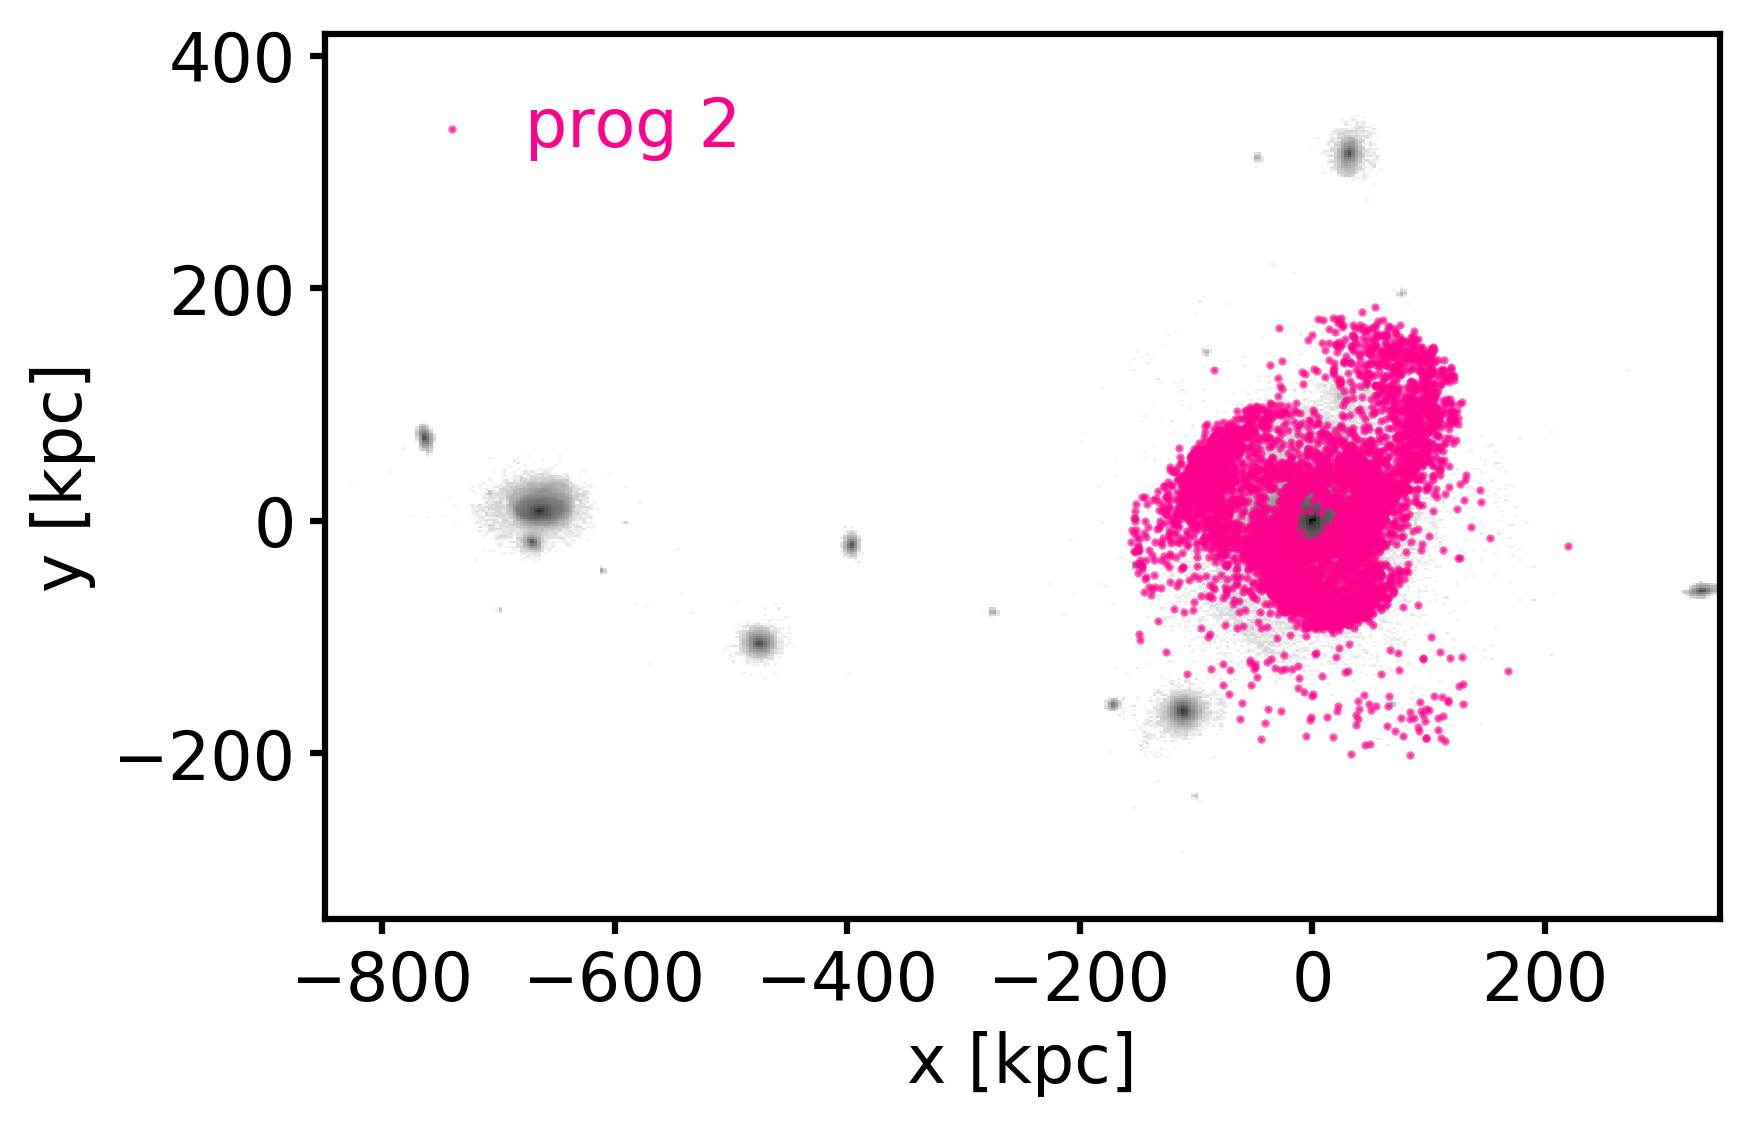
\includegraphics[width=\textwidth]{plots/Dynamics/dist/xy_dist_selected_GCs_prog_2_snap_127.png}
    	\label{fig:prog2_xy}
    \end{subfigure}
    ~ %add desired spacing between images, e. g. ~, \quad, \qquad, \hfill etc. 
    %(or a blank line to force the subfigure onto a new line)
    \begin{subfigure}[c]{0.48\textwidth}
        \centering
    	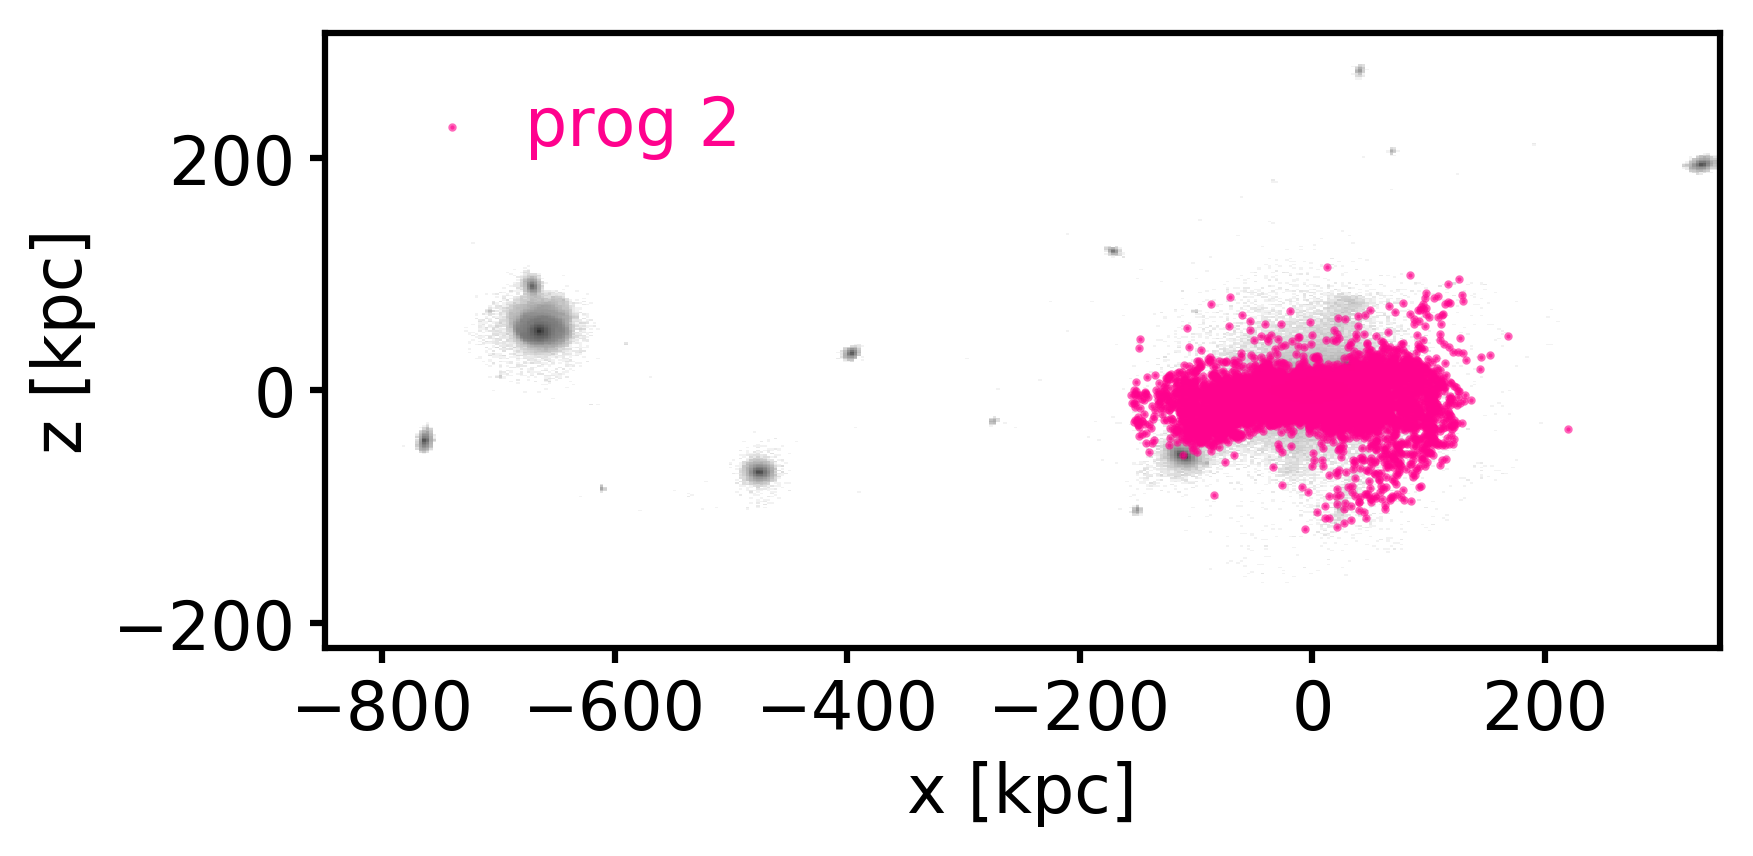
\includegraphics[width=\textwidth]{plots/Dynamics/dist/xz_dist_selected_GCs_prog_2_snap_127.png}
	    \label{fig:prog2_xz}
    \end{subfigure}
    
    \begin{subfigure}[c]{0.48\textwidth}
    \centering
    	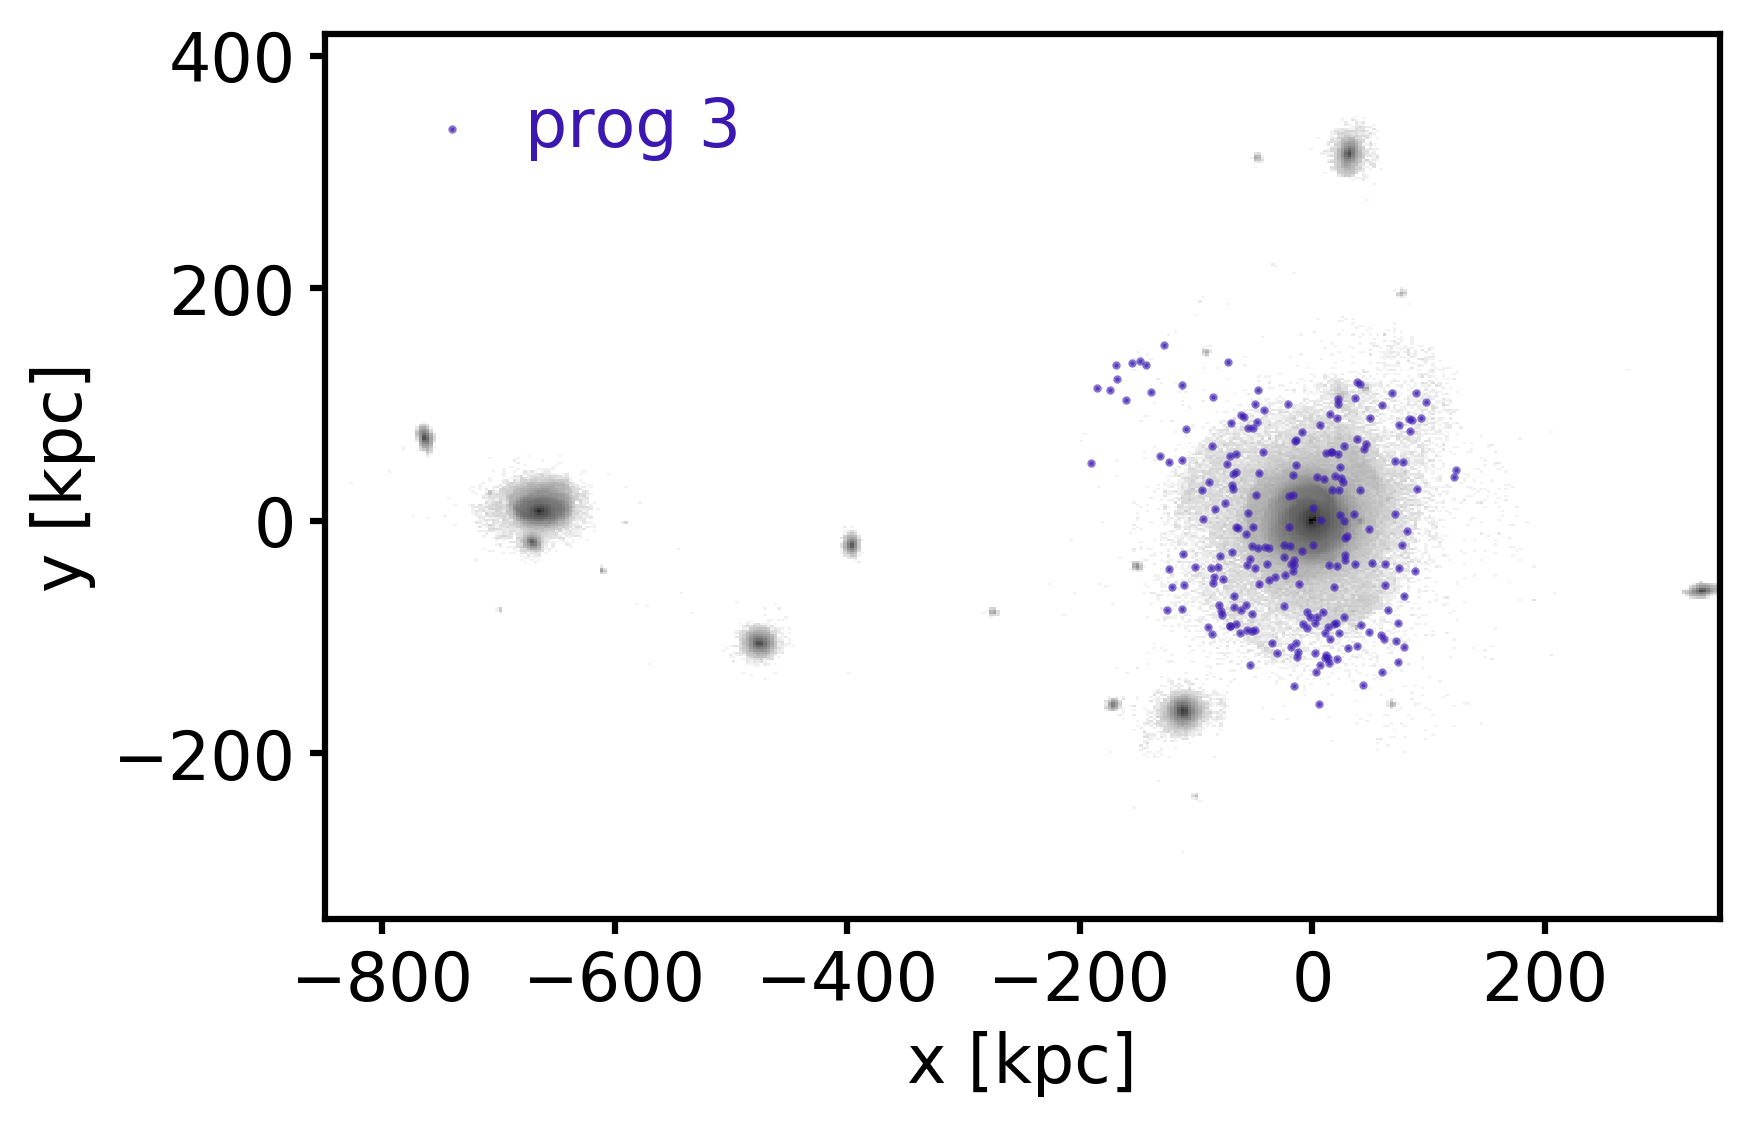
\includegraphics[width=\textwidth]{plots/Dynamics/dist/xy_dist_selected_GCs_prog_3_snap_127.png}
    	\label{fig:prog3_xy}
    \end{subfigure}
    ~ %add desired spacing between images, e. g. ~, \quad, \qquad, \hfill etc. 
    %(or a blank line to force the subfigure onto a new line)
    \begin{subfigure}[c]{0.48\textwidth}
        \centering
    	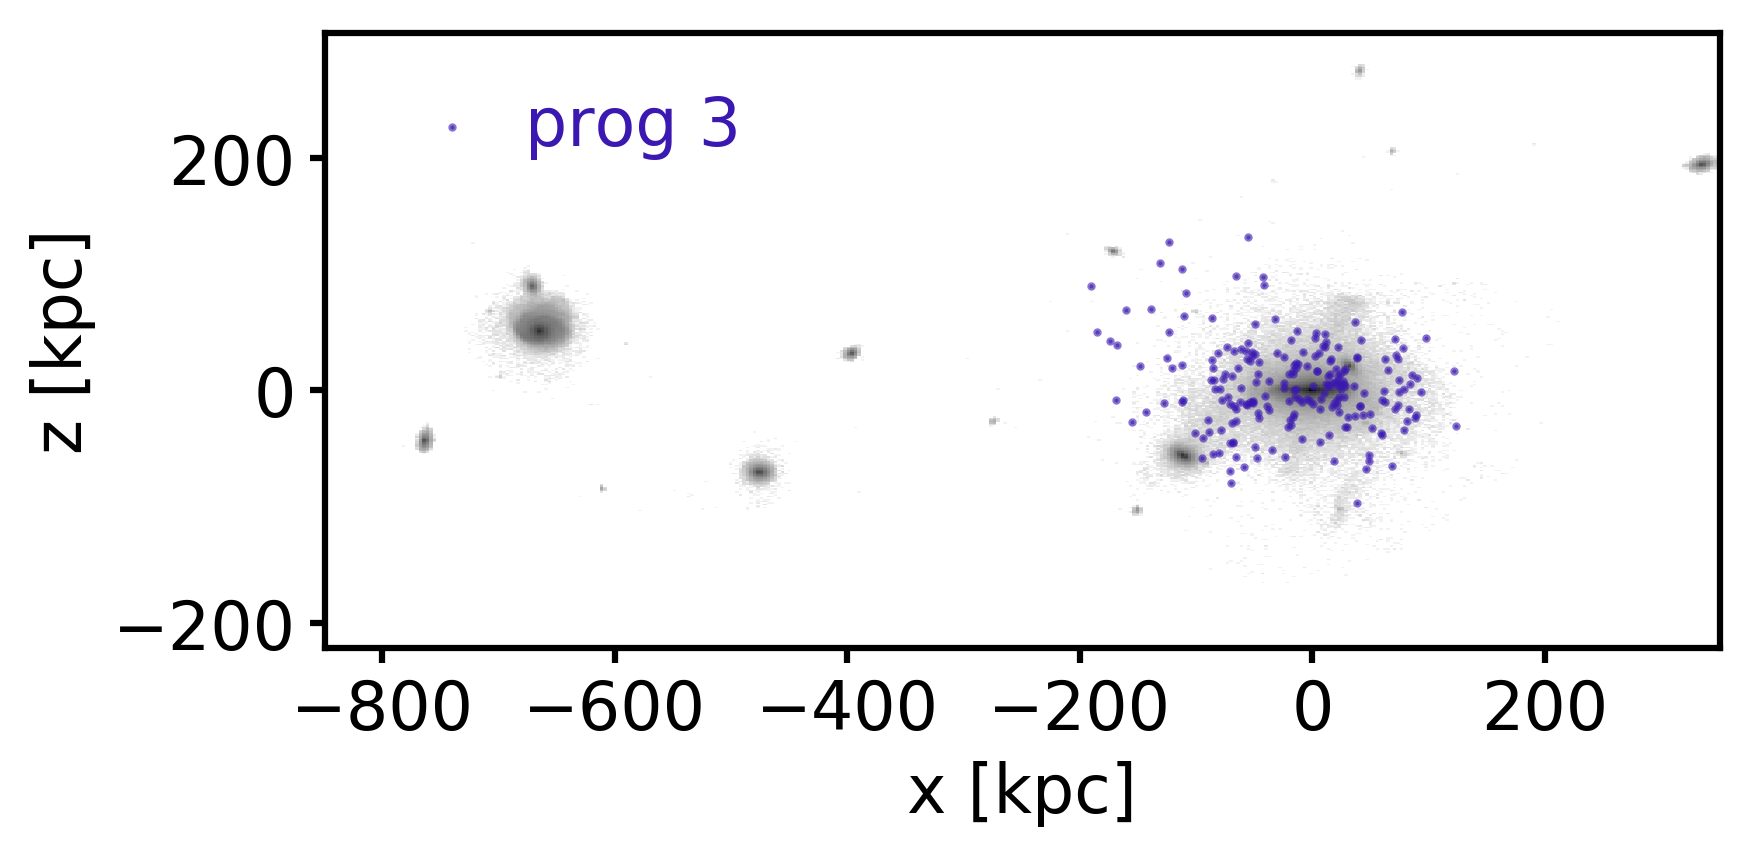
\includegraphics[width=\textwidth]{plots/Dynamics/dist/xz_dist_selected_GCs_prog_3_snap_127.png}
	    \label{fig:prog3_xz}
    \end{subfigure}
    
    \begin{subfigure}[c]{0.48\textwidth}
    \centering
    	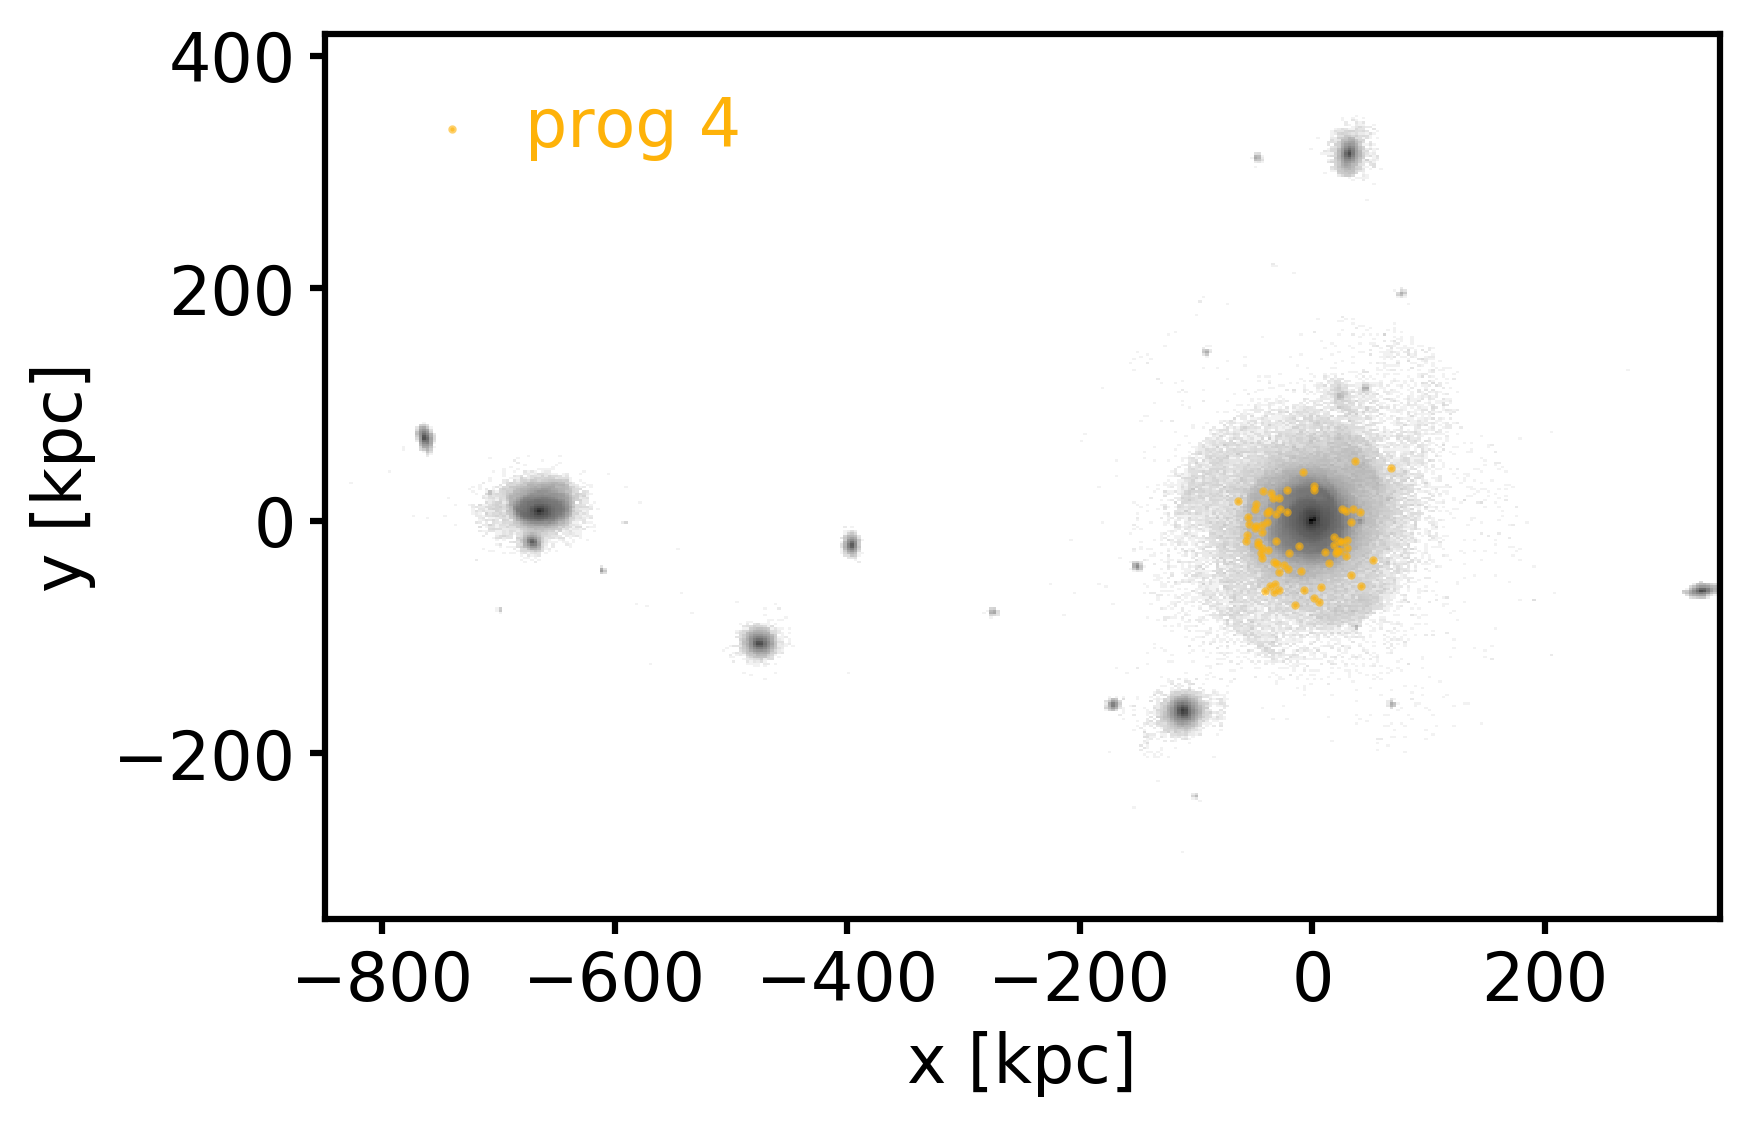
\includegraphics[width=\textwidth]{plots/Dynamics/dist/xy_dist_selected_GCs_prog_4_snap_127.png}
    	\label{fig:prog4_xy}
    \end{subfigure}
    ~ %add desired spacing between images, e. g. ~, \quad, \qquad, \hfill etc. 
    %(or a blank line to force the subfigure onto a new line)
    \begin{subfigure}[c]{0.48\textwidth}
        \centering
    	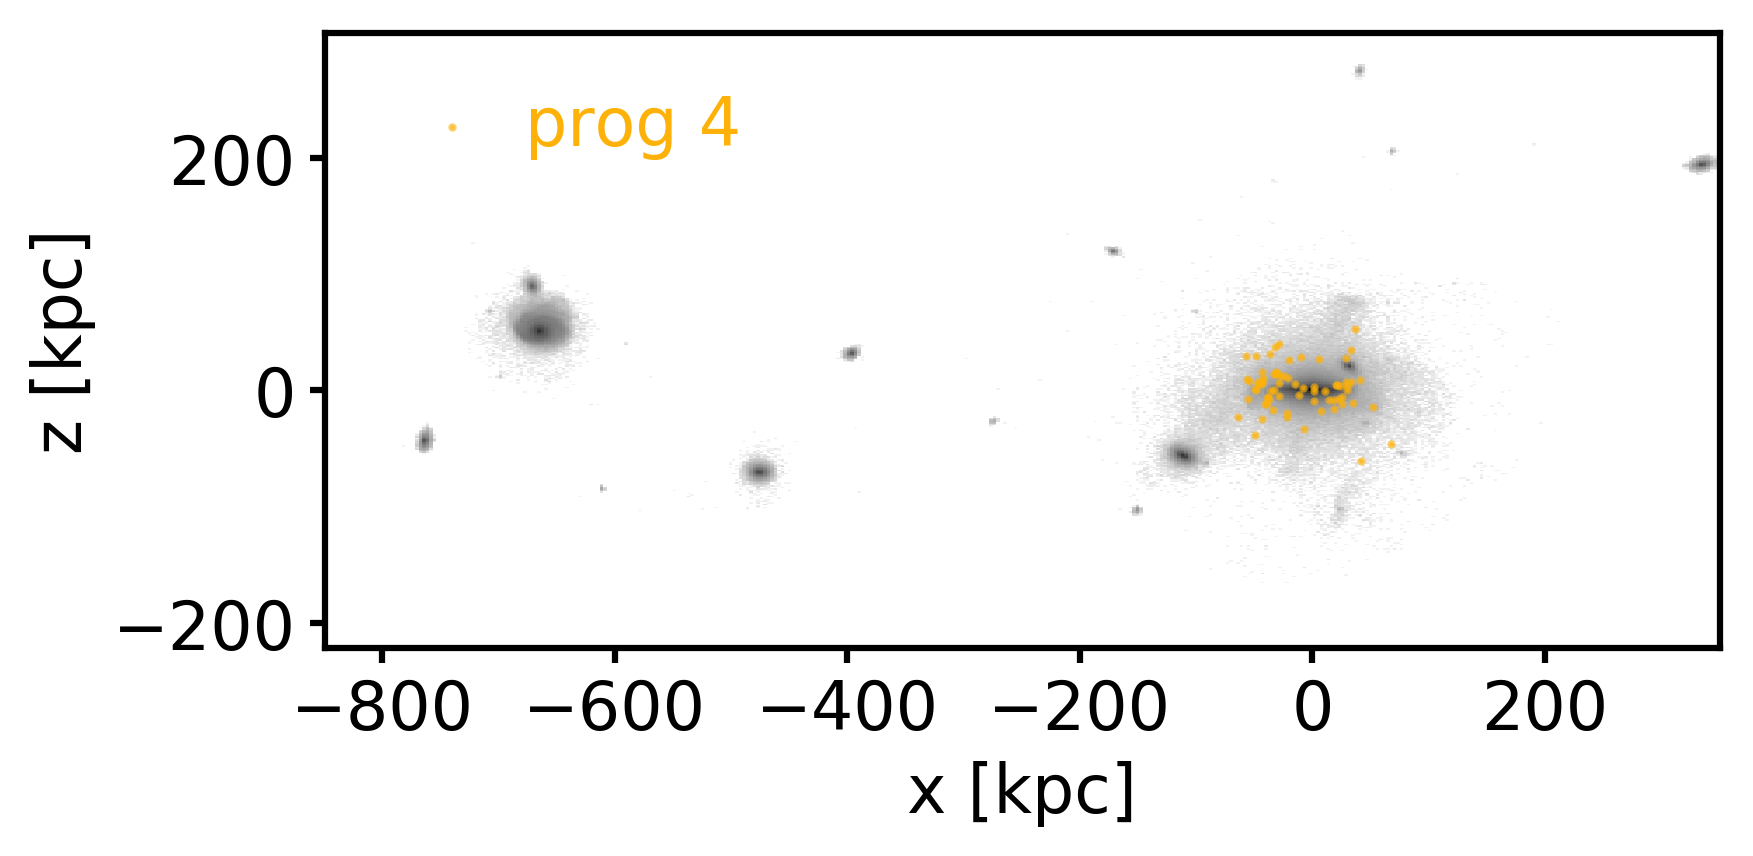
\includegraphics[width=\textwidth]{plots/Dynamics/dist/xz_dist_selected_GCs_prog_4_snap_127.png}
	    \label{fig:prog4_xz}
    \end{subfigure}
    \caption{Remnants of the three biggest \ac{DG} mergers which were not destroyed by the disk. The left panels show the x-y number distribution, the right panels the x-z distribution. In grey, the main galaxy and its satellites are plotted (as in Figure \ref{fig:Stars_AU24}). \textit{Upper panels}: The remnants of the most recent merger are plotted in pink. \textit{Middle panel}: The blue points are remnants of the second biggest merger. \textit{Lower panel}: The yellow points are remnants of the third biggest merger which is the most long ago of these three. These remnants will be considered the \ac{GC} populations of each merger event.}\label{fig:progenitors_distribution}
\end{figure}
The positions of the remnants of these three merger events are shown in Figure \ref{fig:progenitors_distribution}. Progenitor 3 and 4 are totally dispersed in the galaxy while progenitor 2 still shows some merging features such as broad streams, especially visible face-on. Progenitor 2 has nearly a factor of 100 more remaining \acp{GC} than the other two progenitors. This is due to the short time it is in the main galaxy and therefore could these \acp{GC} are neither as much dissolved as the others nor as much disrupted by the disk. Since these three mergers are so different at redshift 0, it is interesting to test their behaviour in action space, where dynamical features are expected to be visible longer. 

\subsection{Globular clusters in action space}\label{subsec:GCs_action_space}
Now, we look at the \ac{GC} distribution in action space. Our assumption is that in the "true" potential, \acp{GC} are very clumped since they should retain dynamical memory from their former \ac{DG} and therefore their \ac{DF} should be a delta function. In section \ref{subsubsec:GCs_actions_right_pot}, we will look at the distribution in the fitted potential at redshift 0. In section \ref{subsubsec:GCs_actions_varying_pot}, we evaluate actions in varying potentials to test our assumption of \acp{GC} being most clumped in action space in the "true" potential. 

\subsubsection{Best fit potential}\label{subsubsec:GCs_actions_right_pot}

\begin{figure}[htbp]
\captionsetup{format=plain}
    \centering
    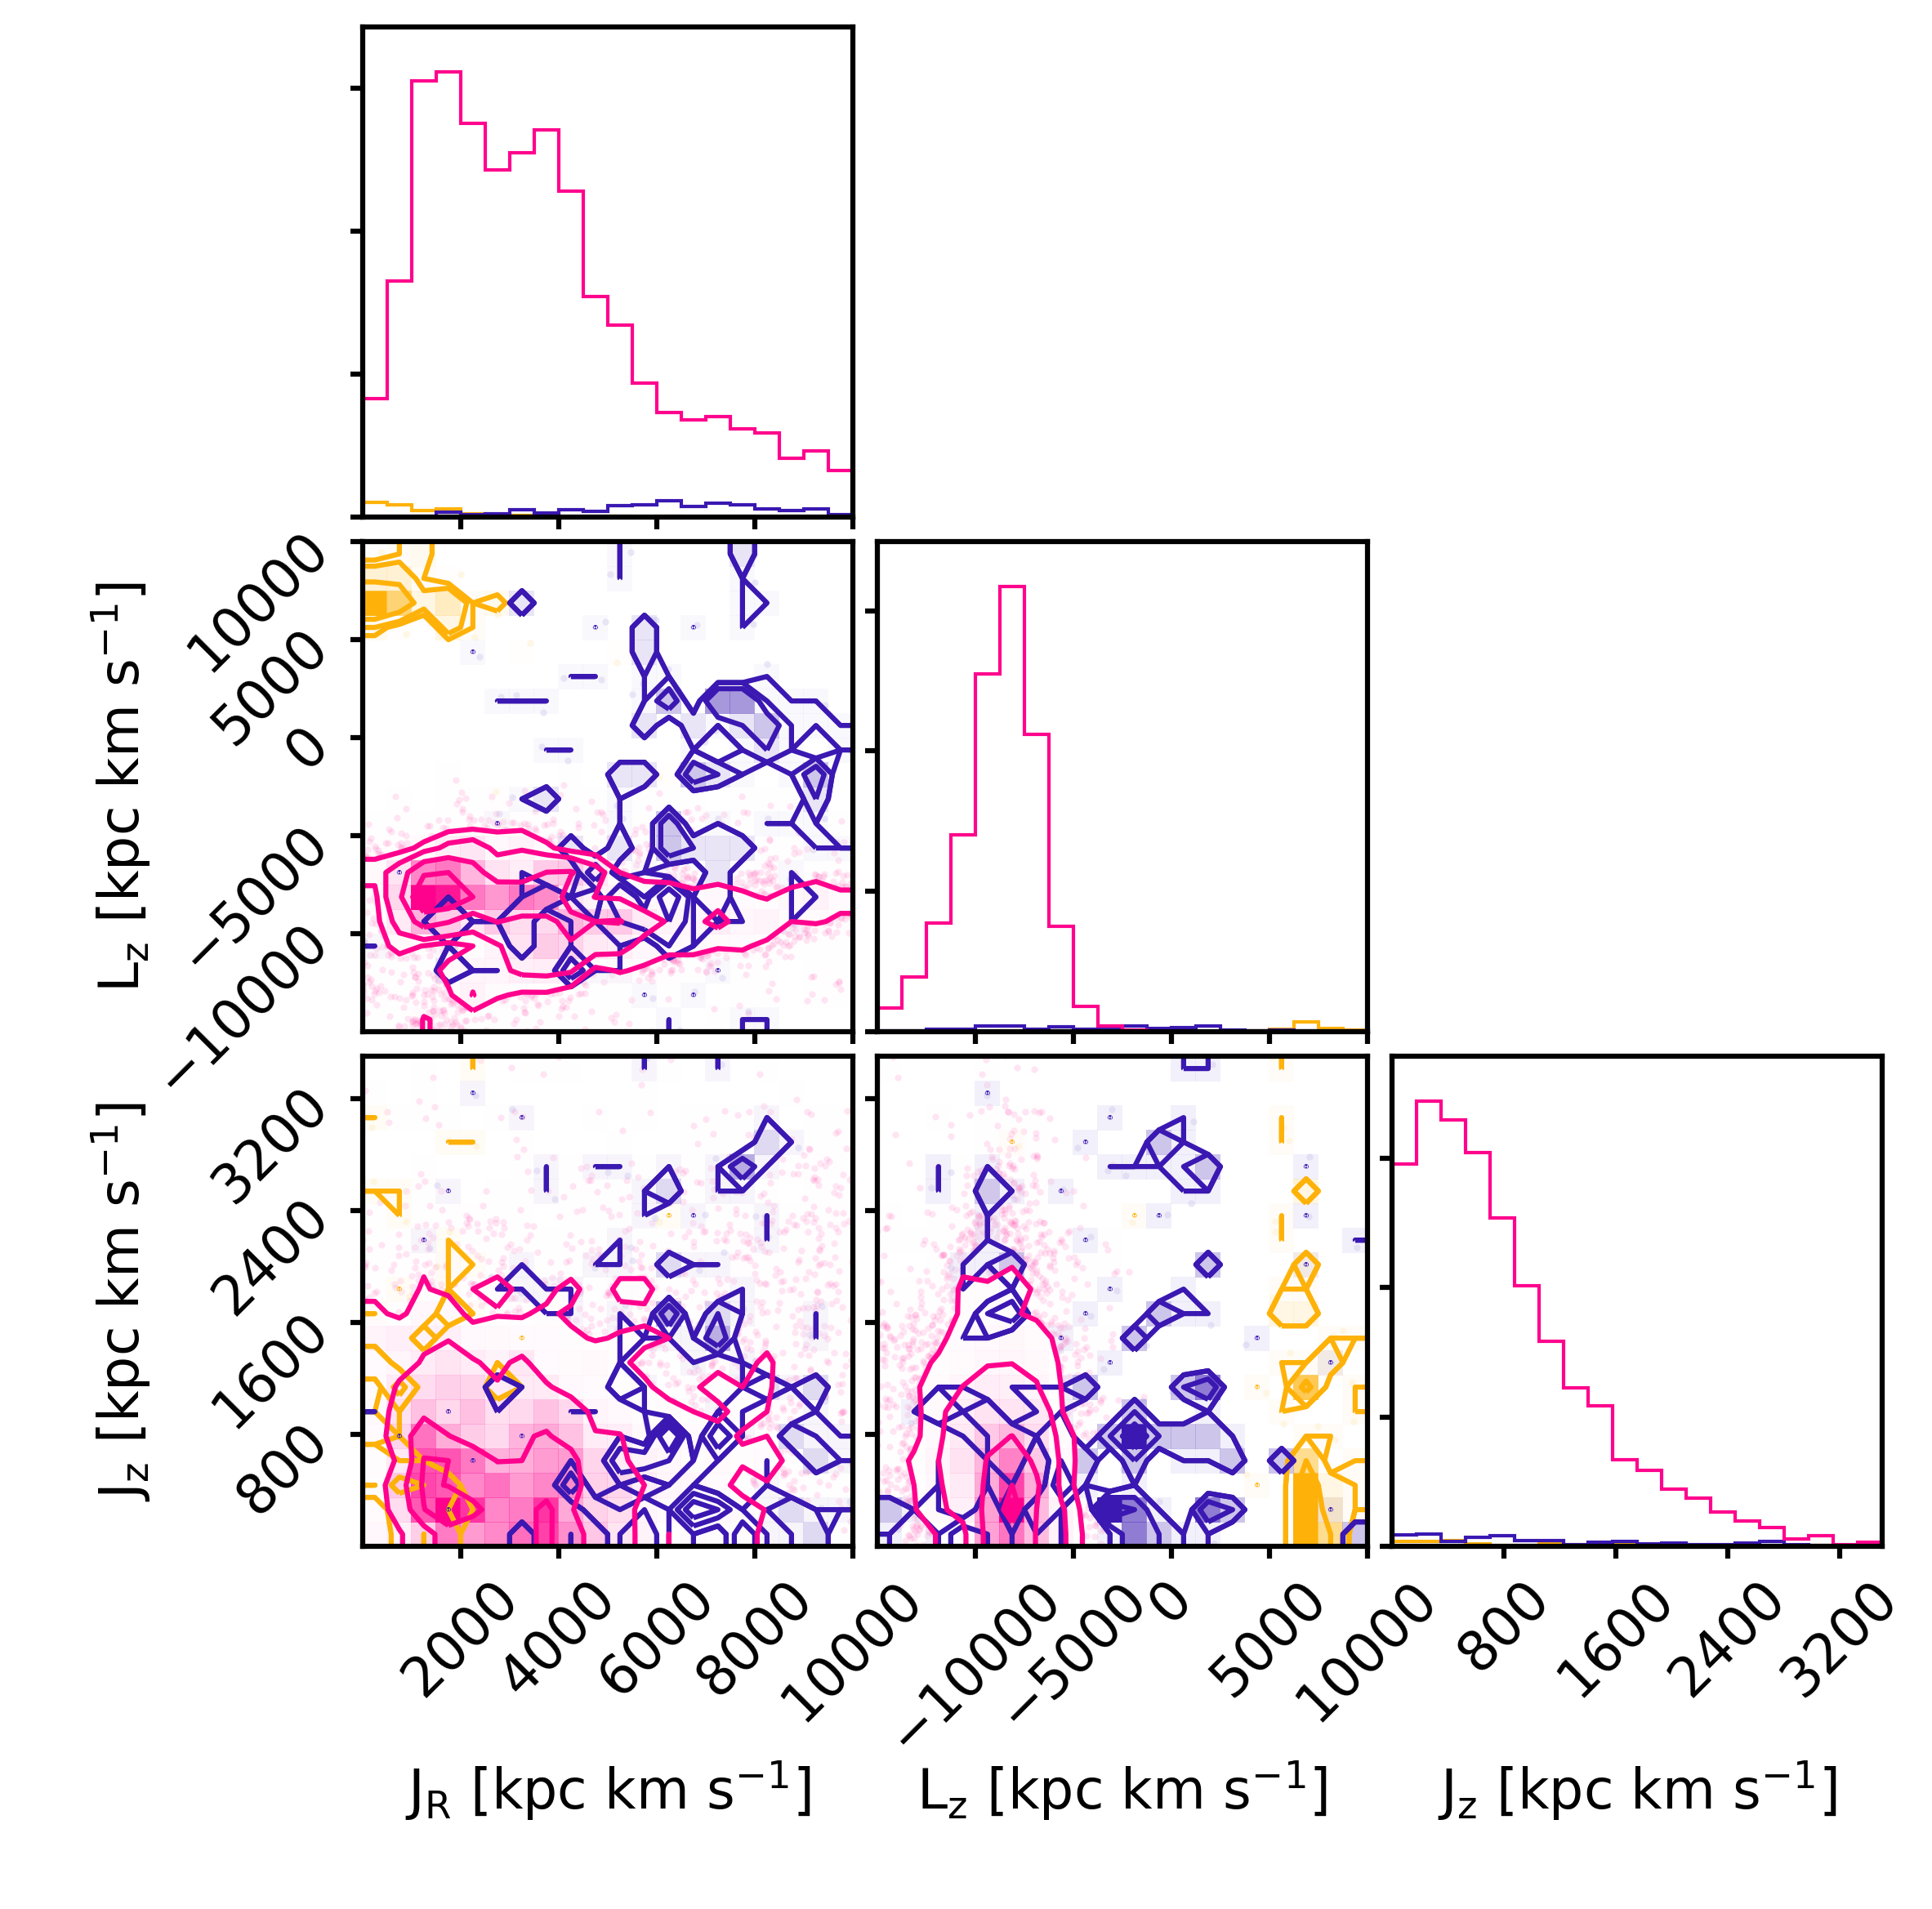
\includegraphics[width=1.0\textwidth]{plots/Dynamics/prog234_actions_snap_127.png}
    \caption{Selected \acp{GC} from three different \acp{DG} in action space. The diagonal elements show histograms of each action and the other panels show 2d histograms of each action pair. In pink/blue/yellow, we see the action distribution of the remnants of prog2/prog3/prog4. Since we have many more particles from prog2, the histograms in the diagonal elements are dominated by their distribution. In the correlation panels, we can clearly distinguish prog 2 and prog 4 while prog 3 is very dispersed and does not have an identifiable center in any action. Even though the merger of prog4 happened the longest ago, it is still very clumped in all combinations, with the most clumpiness in J$_\mathrm{R}$-L$_\mathrm{Z}$. The distribution of prog2 is narrow in L$_\mathrm{Z}$ but very broad in J$_\mathrm{R}$-J$_\mathrm{Z}$. prog2 is corotating with the disk but with a higher angular momentum than the disk has (\(\bar{\mathrm{L_z}} = -2235\) kpc km s$^{-1}$). prog4 is clearly counter rotating.}
    \label{fig:act_all_merg_best_pot}
\end{figure}
We calculate the actions of the remnants of each progenitor in the best fit potential and plot them in Figure \ref{fig:act_all_merg_best_pot}. The remnants of the different merger events are best distinguishable in L$_\mathrm{Z}$. Prog2 is corotating with the disk but with higher angular momentum. Prog4 is counter rotating. Prog3 is more dispersed in L$_\mathrm{Z}$ but its mean is corotating with the disk as well. In the vertical action, the three remnant groups are not distinguishable and have means at \SI{1000-2000}{kpc.km.s^{-1}}. In J$_\mathrm{R}$, the groups are again distinguishable. 
\\The idea of this method is that in the right potential, these groups minimize their spread in action space. Prog4 is the most compact group, while especially prog3 is very dispersed. To quantify the compactness, we measure the standard deviation of each action. In the next Section, we compare the standard deviations of the radial and vertical actions of each group in different potentials to see, if we minimize them in the 'true' potential.

\subsubsection{Varying potentials}\label{subsubsec:GCs_actions_varying_pot}
To vary the potential in way it should affect the groups the most, we vary the \ac{DM} halo. We do this by keeping all best fit potential parameters constant and only vary the scale length a$_\mathrm{NFW}$. For the three groups in these potentials, we calculate the actions in the $z=0$ snapshot.
\begin{figure}[!ht]
\captionsetup{format=plain}
   \subfloat{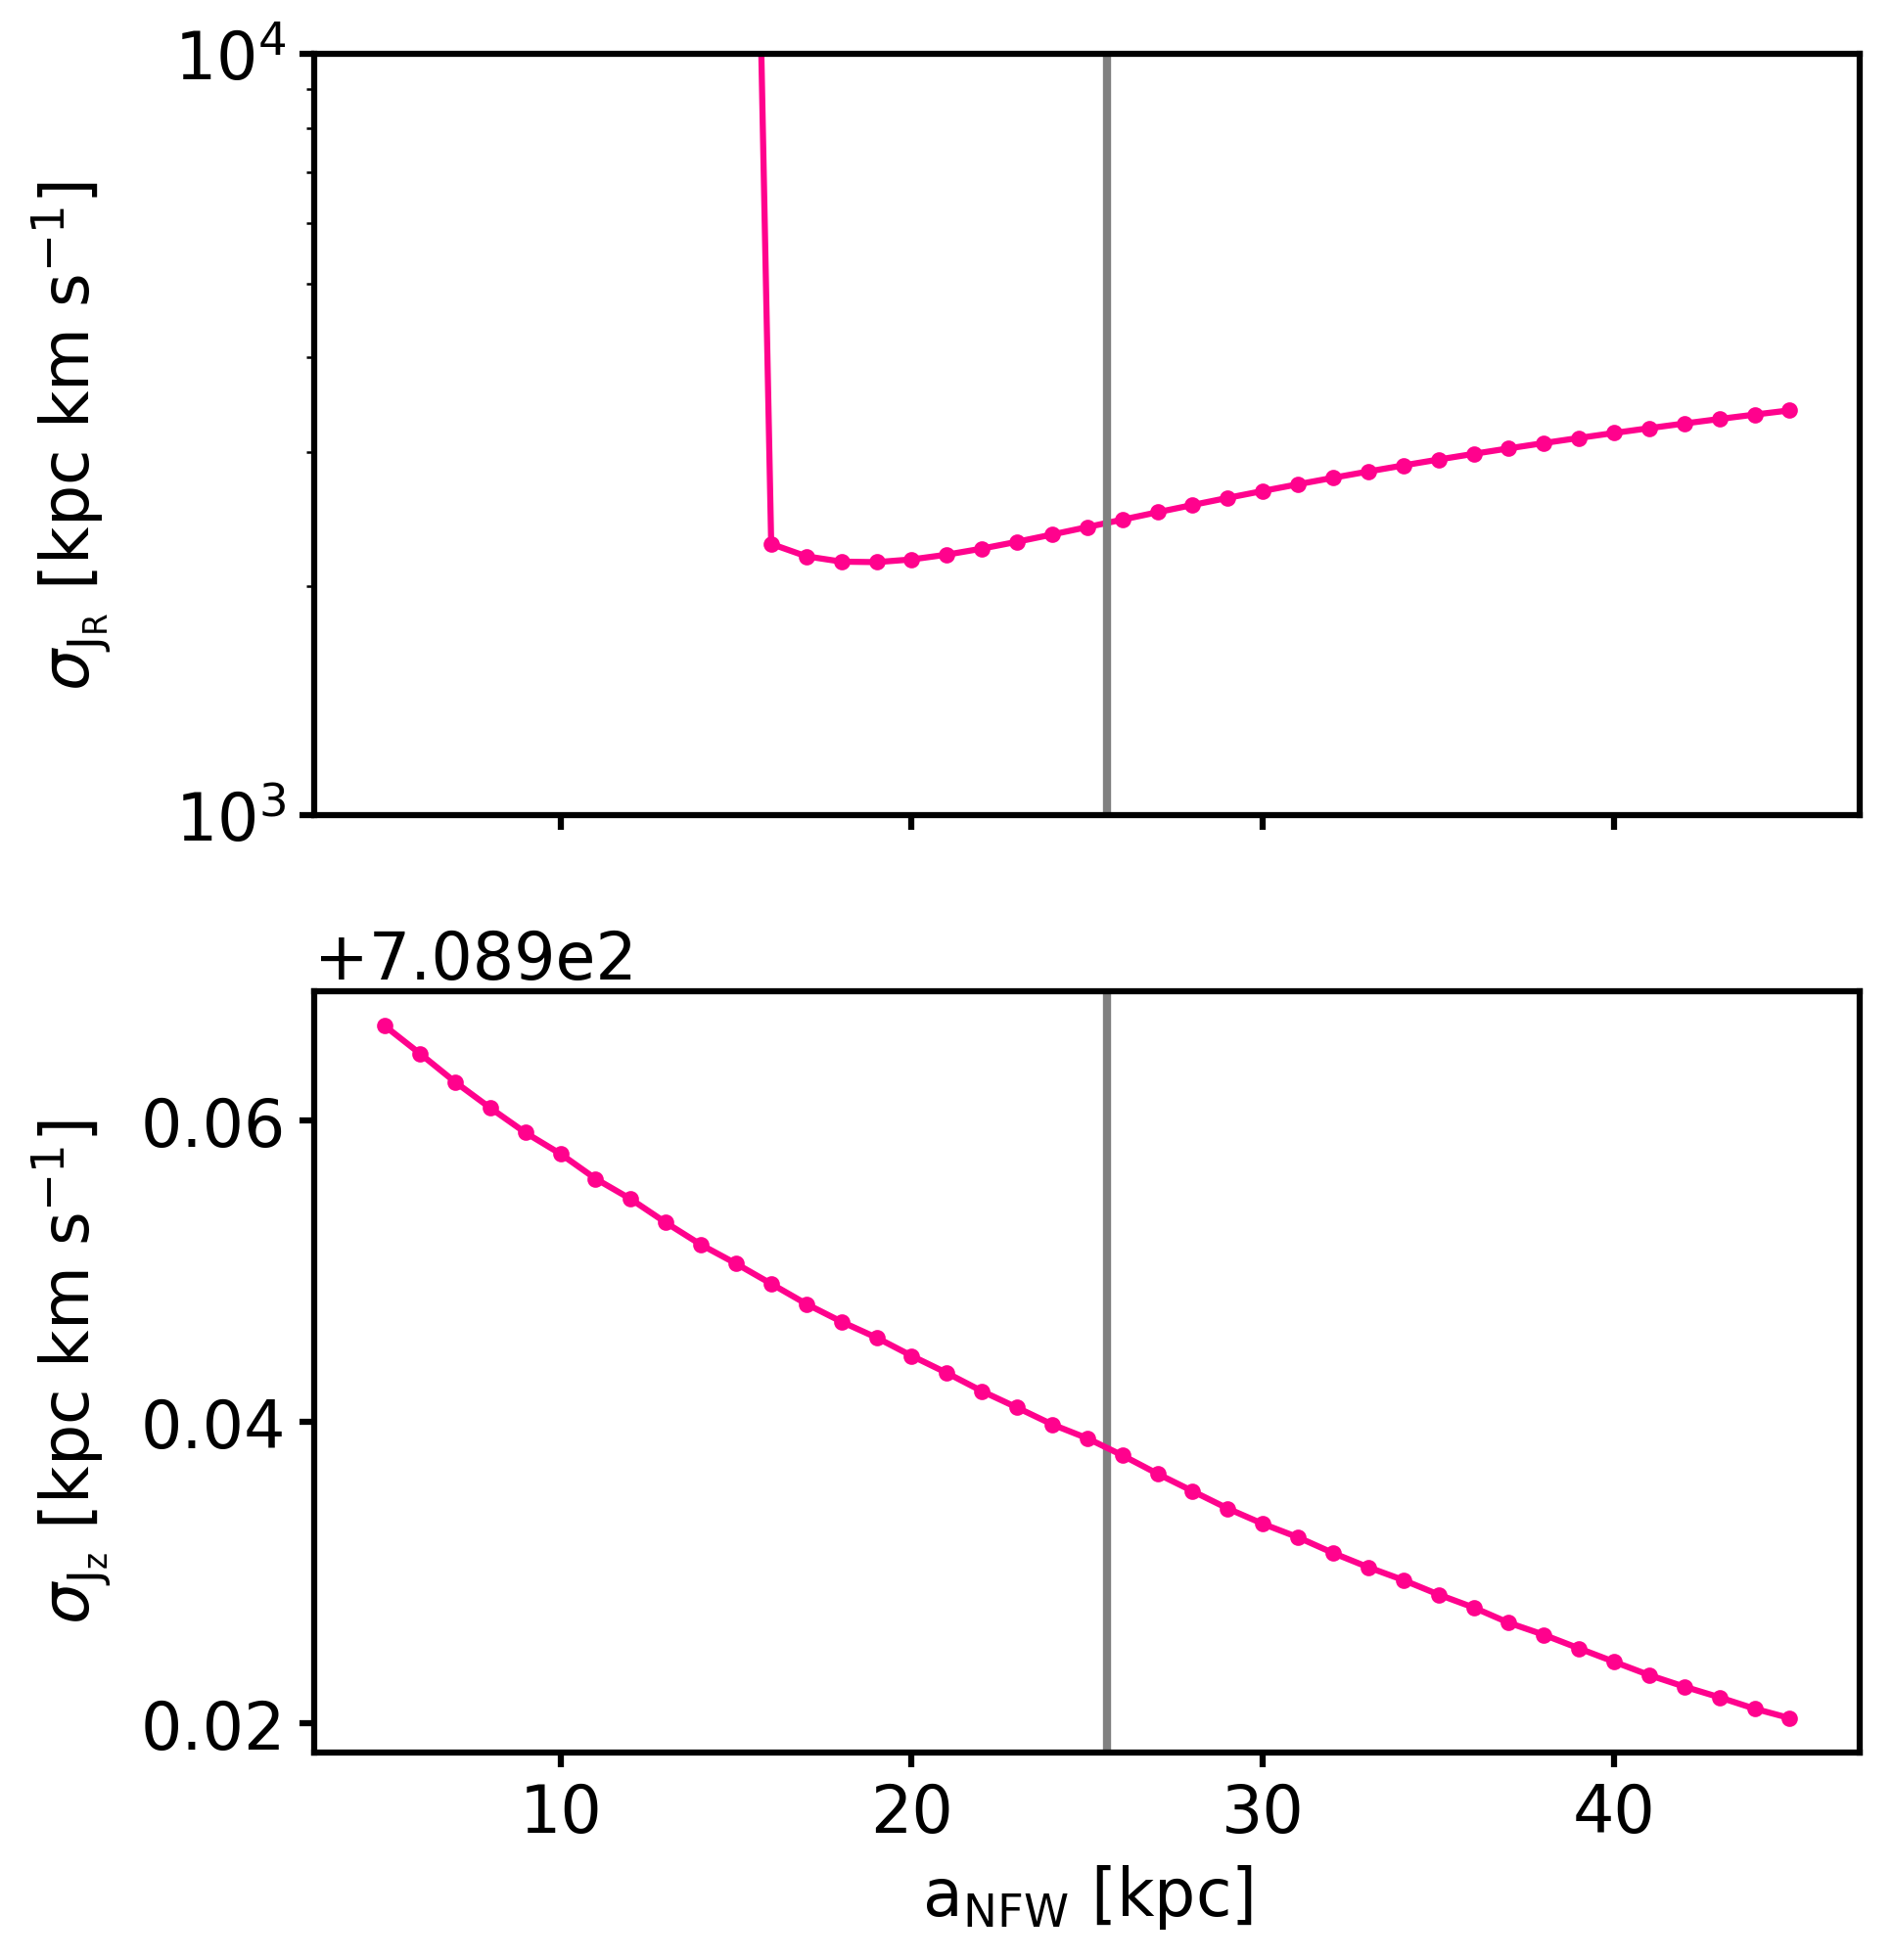
\includegraphics[width=0.48\textwidth]{plots/Dynamics/prog2/a_NFW_diagnostic_plot_std_prog2_all.png}}\hfill%
   \subfloat{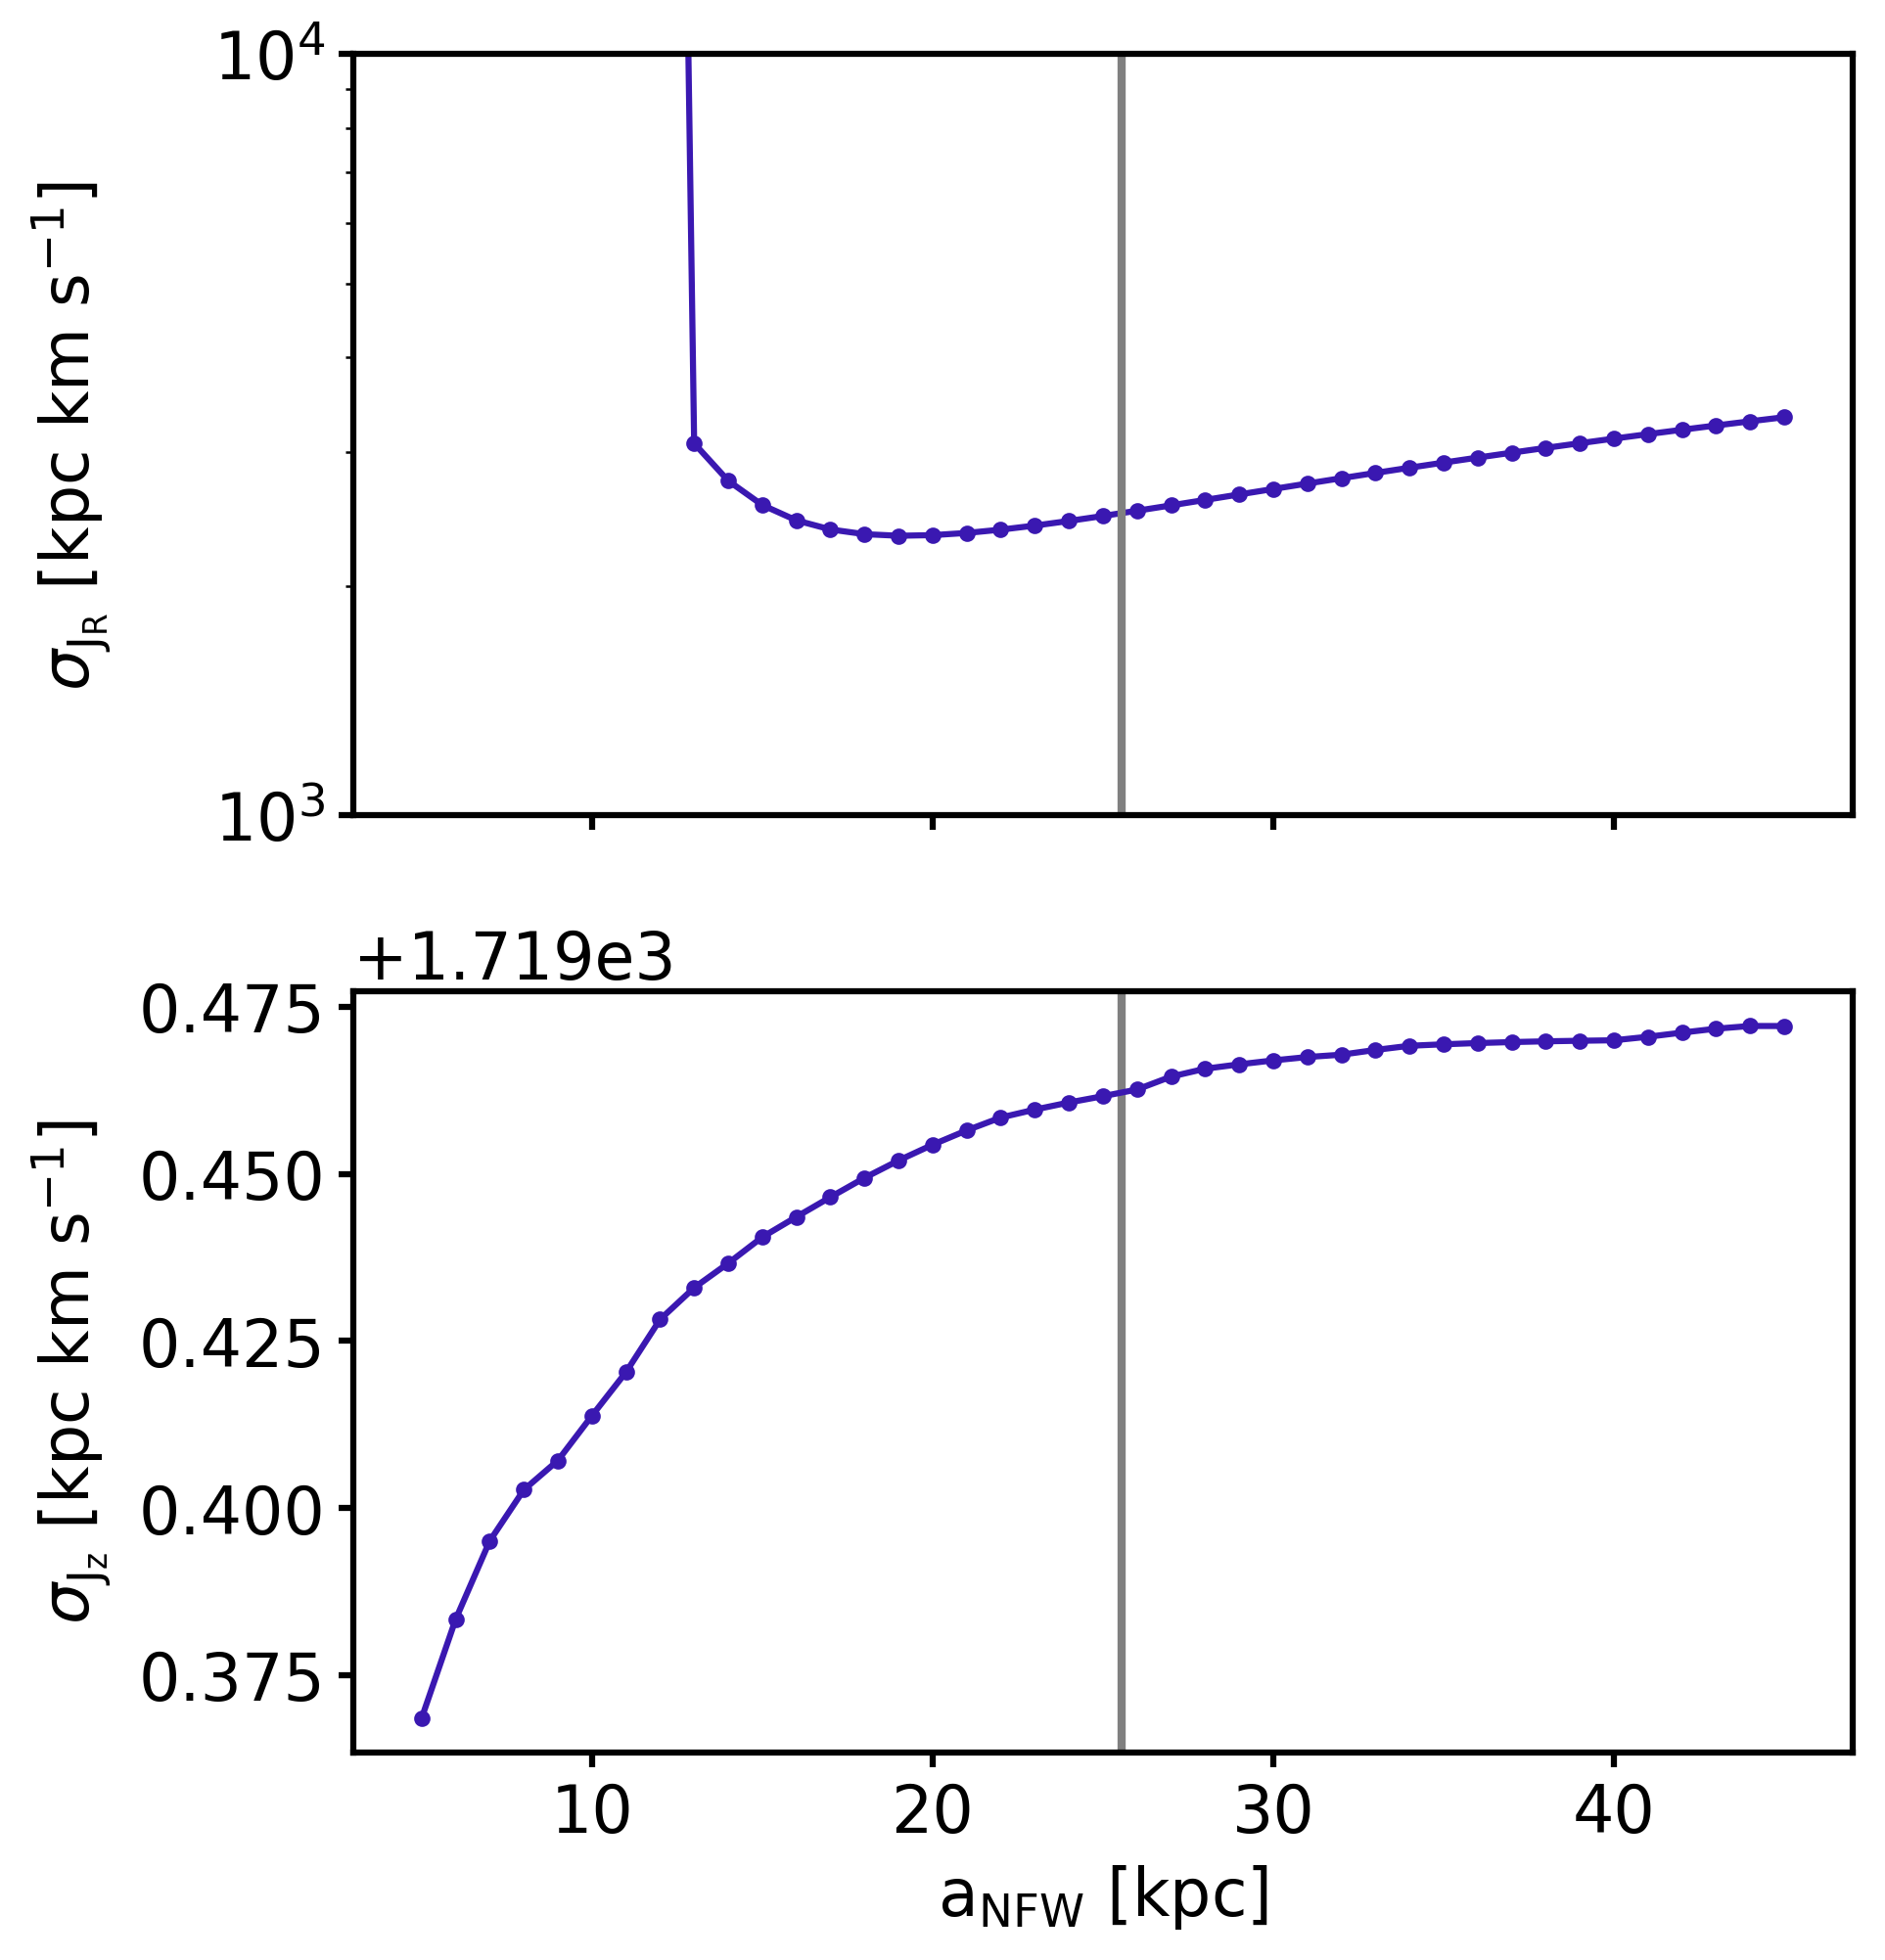
\includegraphics[width=0.48\textwidth]{plots/Dynamics/prog3/a_NFW_diagnostic_plot_std_prog3_all.png}}\vspace*{0.5cm}\par
   \subfloat{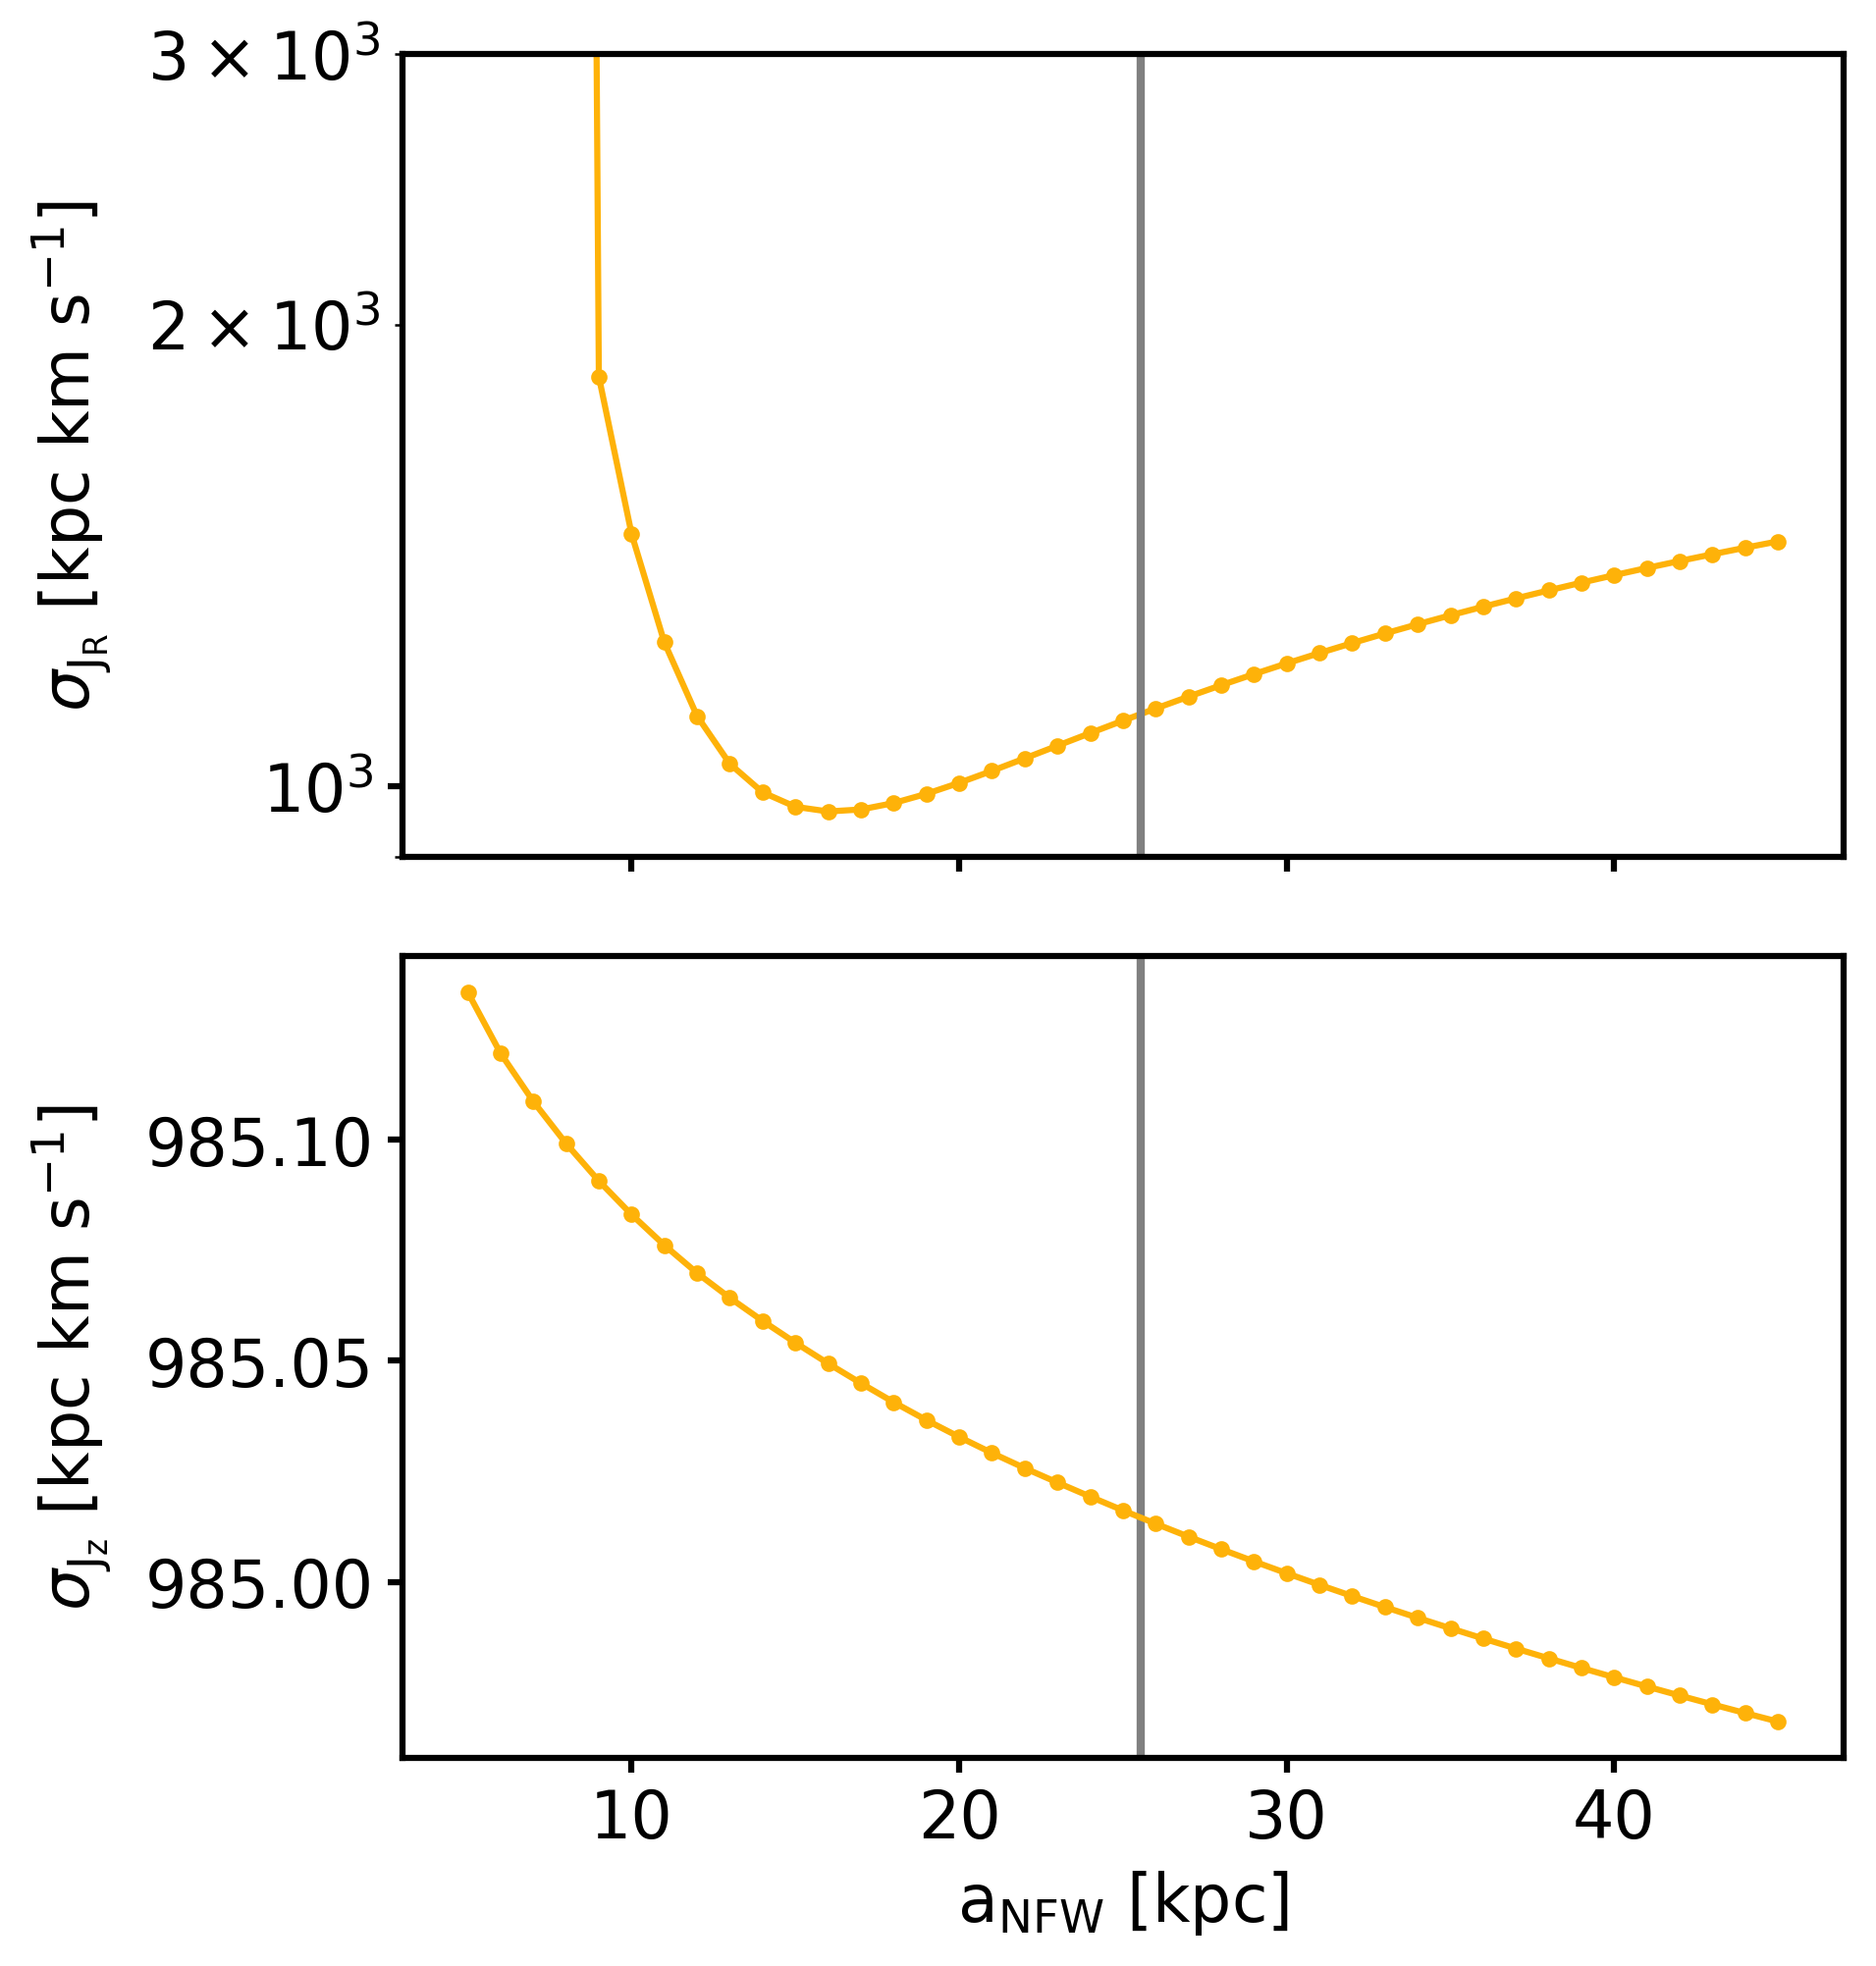
\includegraphics[width=0.48\textwidth]{plots/Dynamics/prog4/a_NFW_diagnostic_plot_std_prog4_all.png}}\hfill%
   \parbox[b][.3\textheight]{.48\textwidth}%
     {\vskip-\abovecaptionskip\RawCaption{\caption{Standard deviations of the radial and vertical actions of all three mergers (prog2-pink / prog3-blue / prog4-yellow) in potentials with varying scale length of the \ac{DM} halo and all other parameters kept on their best fit value. We would expect the standard deviation to be mimized at the best fit potential which is indicated with the vertical grey line. We see that the radial action would prefer a lower scale length (at \SI{17}{kpc}) while two of the three vertical actions would prefer higher scale lengths. The differences in $\sigma_\mathrm{J_z}$ are much smaller than the one in $\sigma_\mathrm{J_R}$.}\vfill\label{fig:a_NFW_diagnostic_plots}}}
\end{figure}
In Figure \ref{fig:a_NFW_diagnostic_plots}, we see how the standard deviations evolve in the different potentials. 

\subsection{Time evolution of actions}\label{subsec:time_evo_actions}
We evaluate the time evolution of the orbits of the accreted \acp{GC} to how the actions evolved and to see if there was a point - probably shortly after their mergers - where the \acp{GC} were more clumped in action space. We calculate the actions of the selected particles in the best fit potential in each snapshot.  

\subsubsection{Best fit potential}\label{subsubsec:GCs_action_time_right_pot}
\begin{figure}[htbp]
\captionsetup{format=plain}
    \centering
	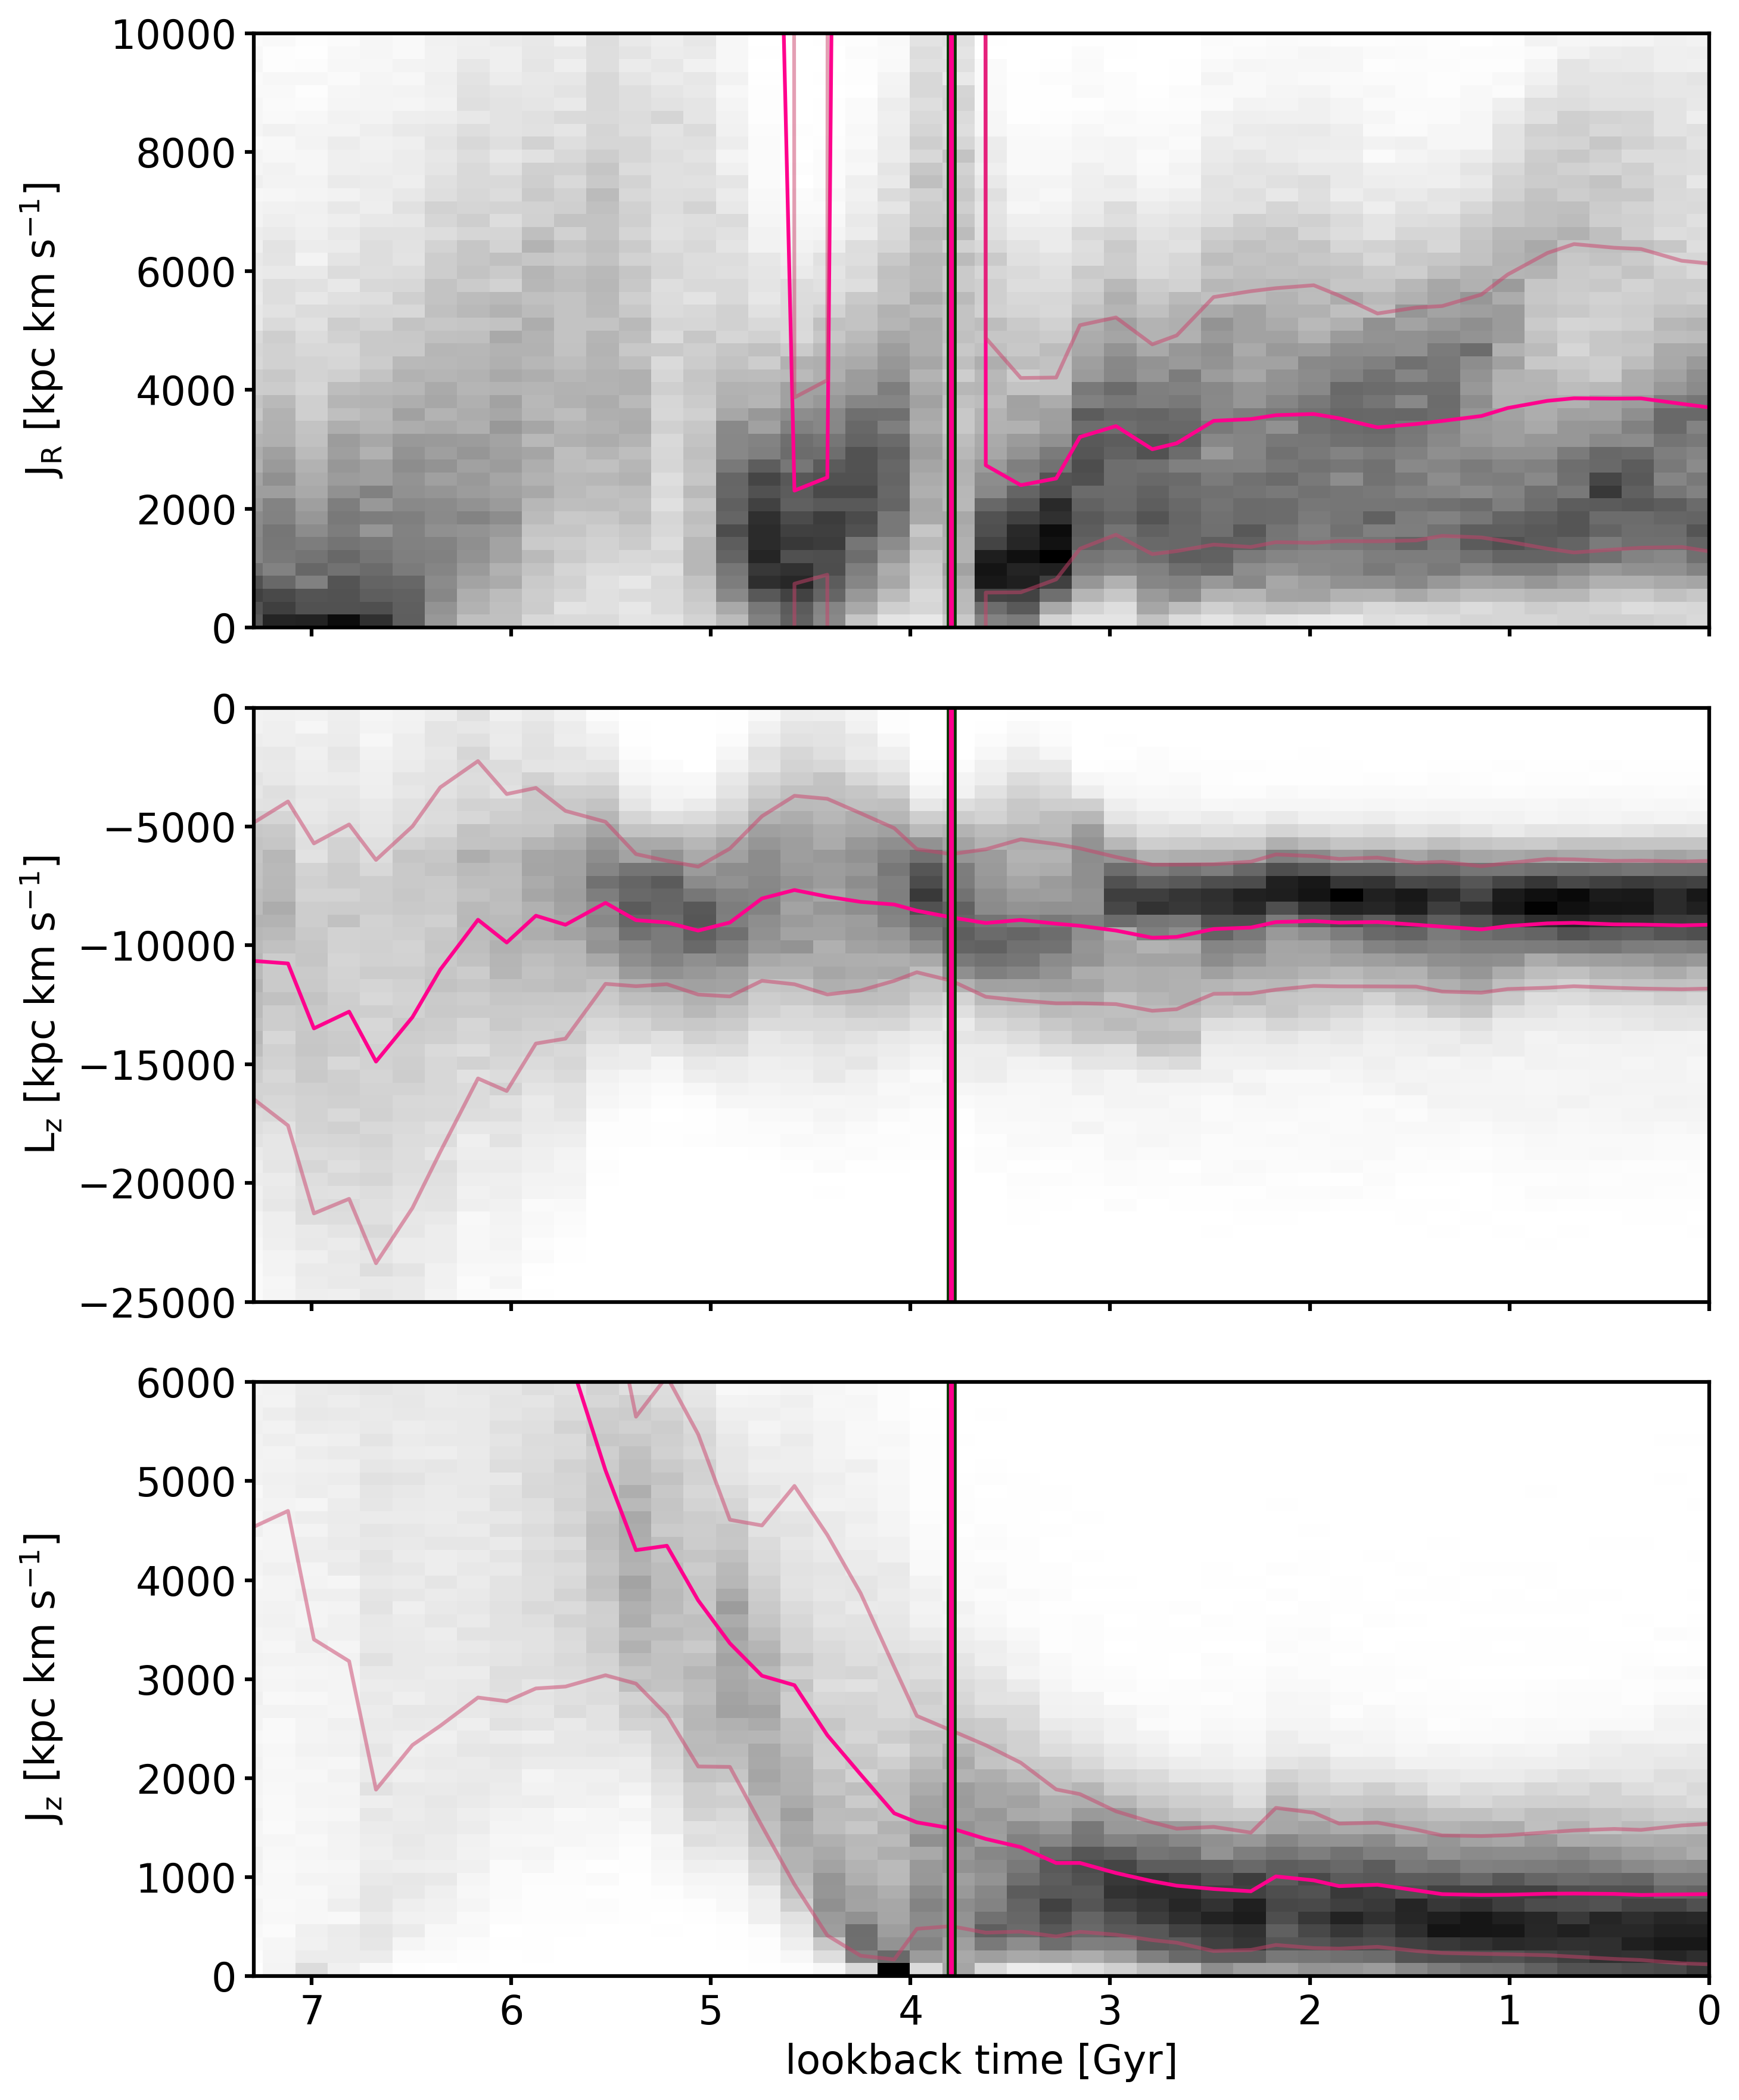
\includegraphics[width=\textwidth]{plots/Dynamics/prog2/action_time_evolution_hist_mean.png}

	\caption{Evolution of actions of prog2 \acp{GC} over time. The pink vertical line indicates the time of the merger. \textit{Upper panel}: Radial action. \textit{Middle panel}: Angular momentum. \textit{Lower panel}: Vertical action. Before the merger, radial and vertical action were much higher and all three actions had higher standard deviations. With the merger, they have settled and L$_\mathrm{Z}$ and J$_\mathrm{Z}$ have a constant mean and standard deviation. J$_\mathrm{R}$ has minimized in mean and standard deviation shortly after the merger but since then both have increased again.}\label{fig:actions_time_evolution_prog2}
\end{figure}

\begin{figure}
\captionsetup{format=plain}
    \centering
	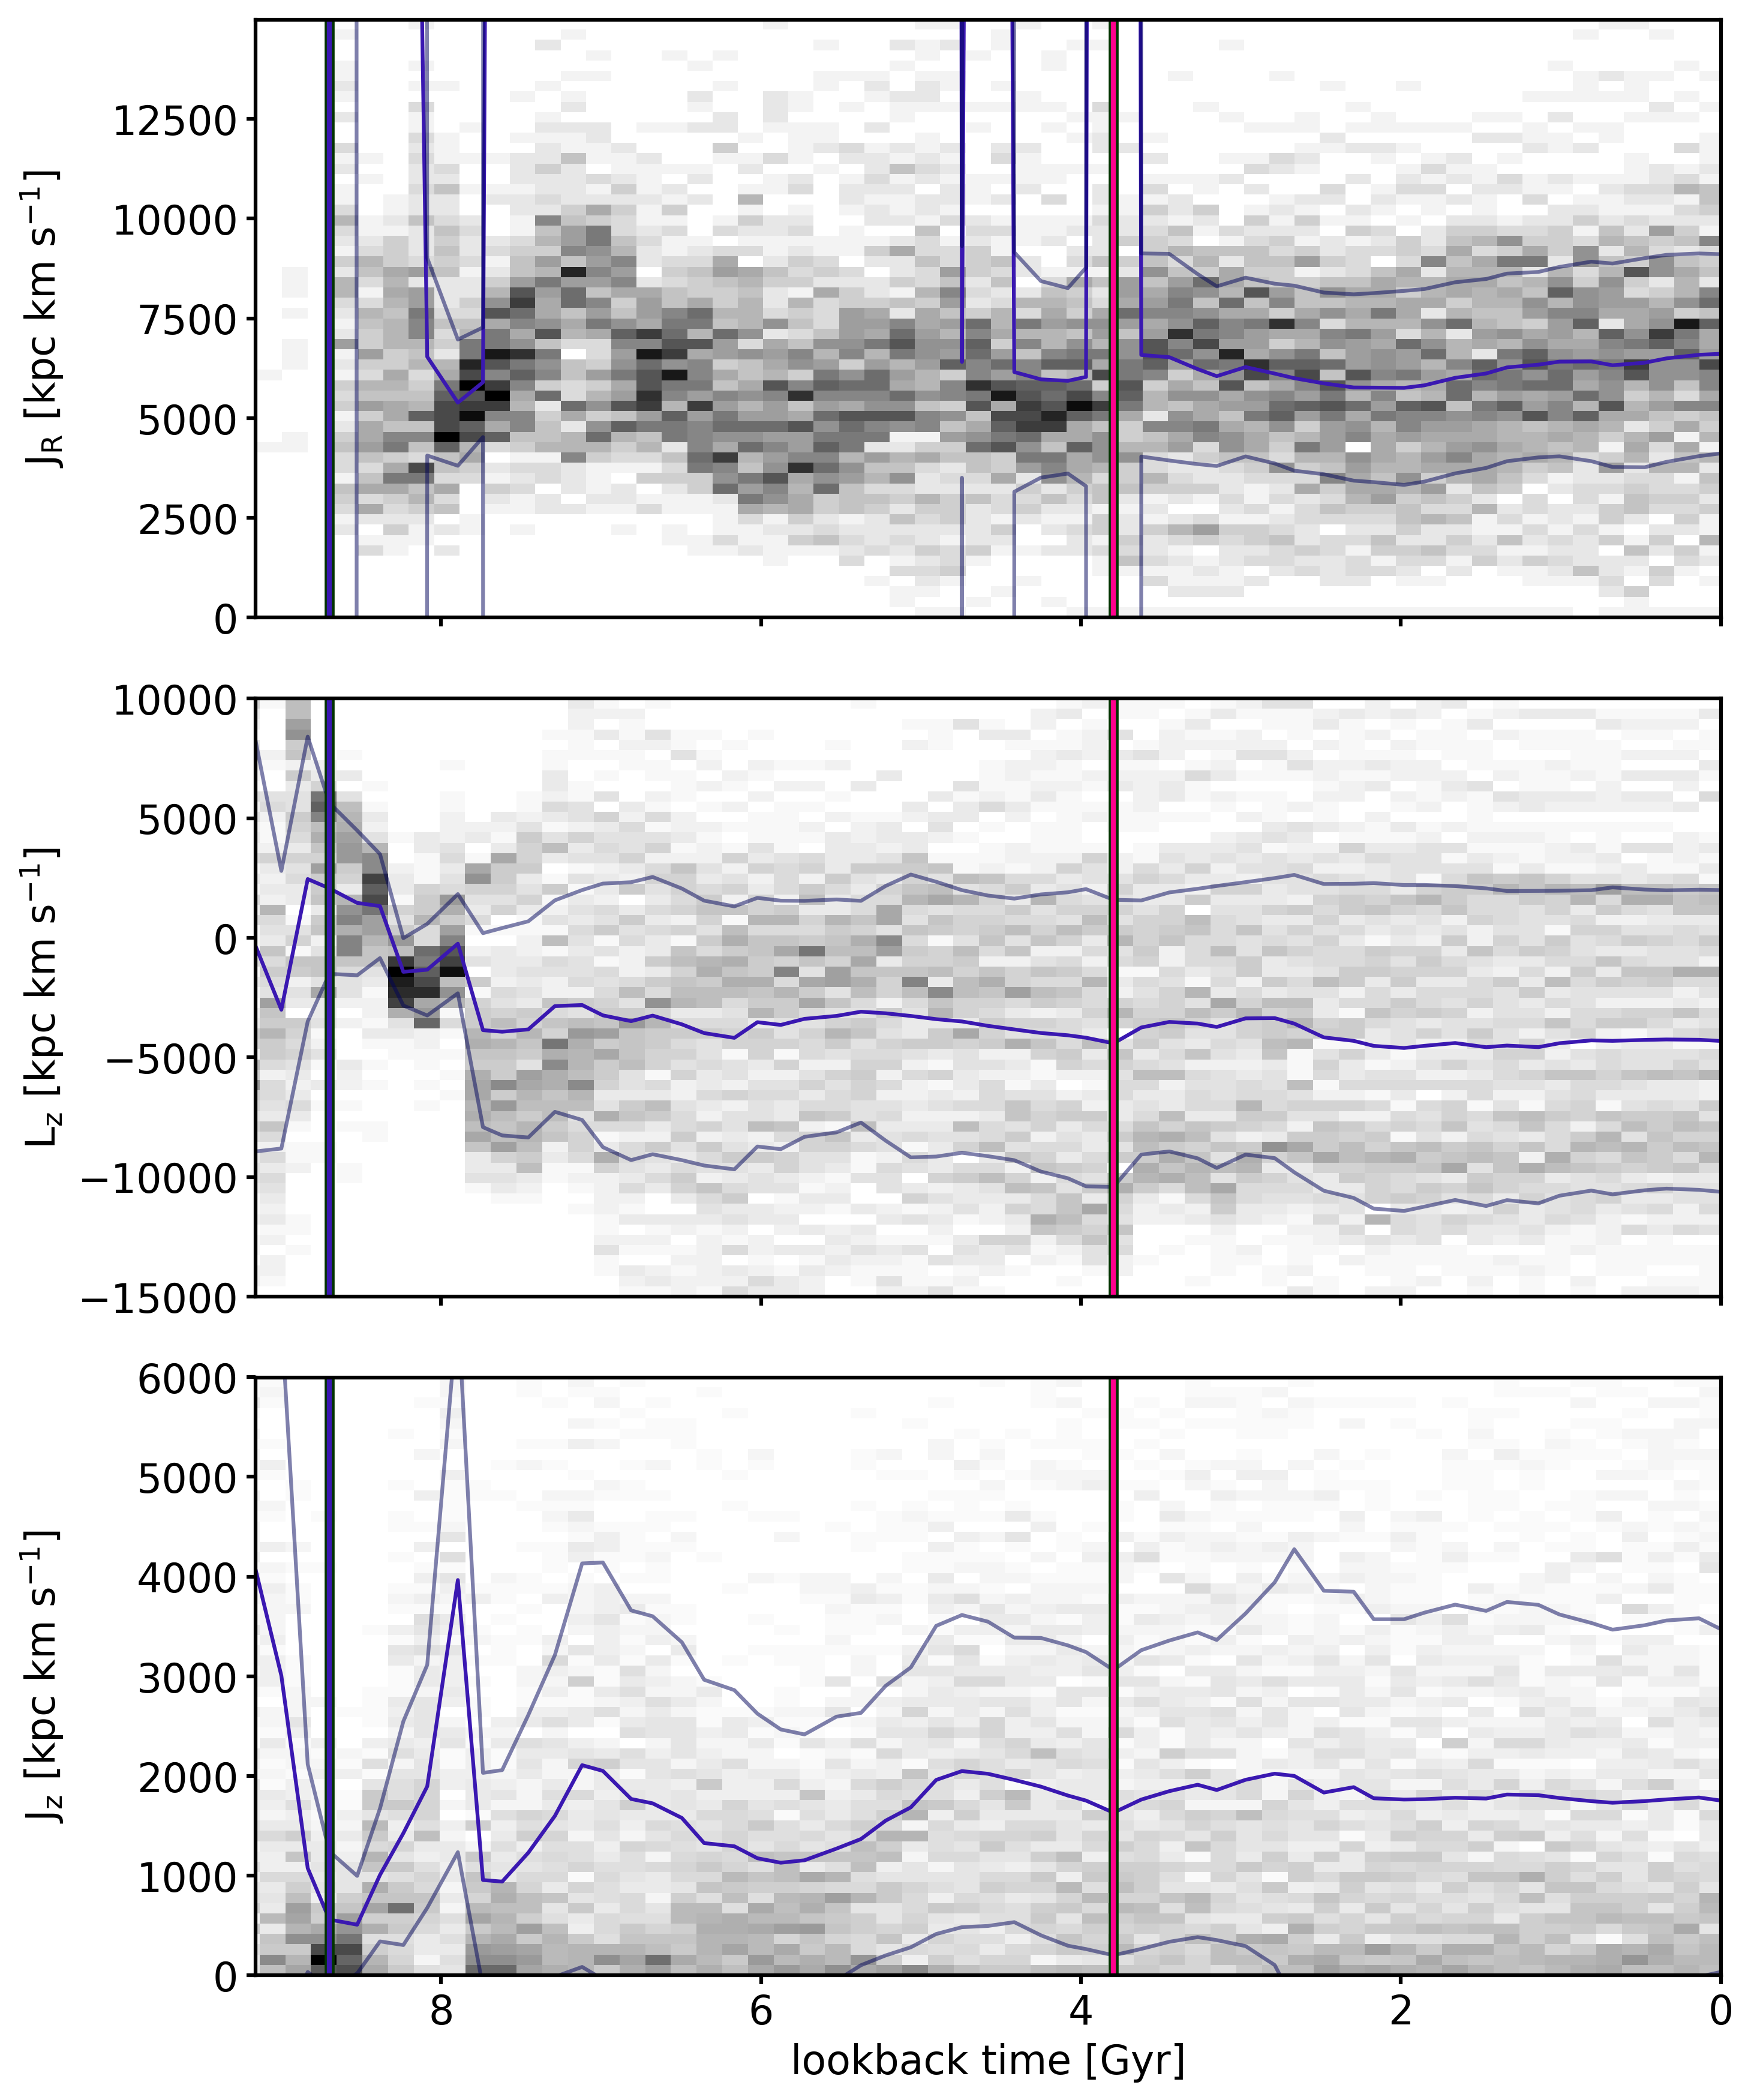
\includegraphics[width=\textwidth]{plots/Dynamics/prog3/action_time_evolution_hist_mean.png}
    \caption{Same as in Figure \ref{fig:actions_time_evolution_prog2}, only for prog3. Now the pink and blue lines indicate times of the mergers of prog2 and prog3, respectively. }\label{fig:actions_time_evolution_prog3}
\end{figure}

\begin{figure}[htbp]
\captionsetup{format=plain}
    \centering
	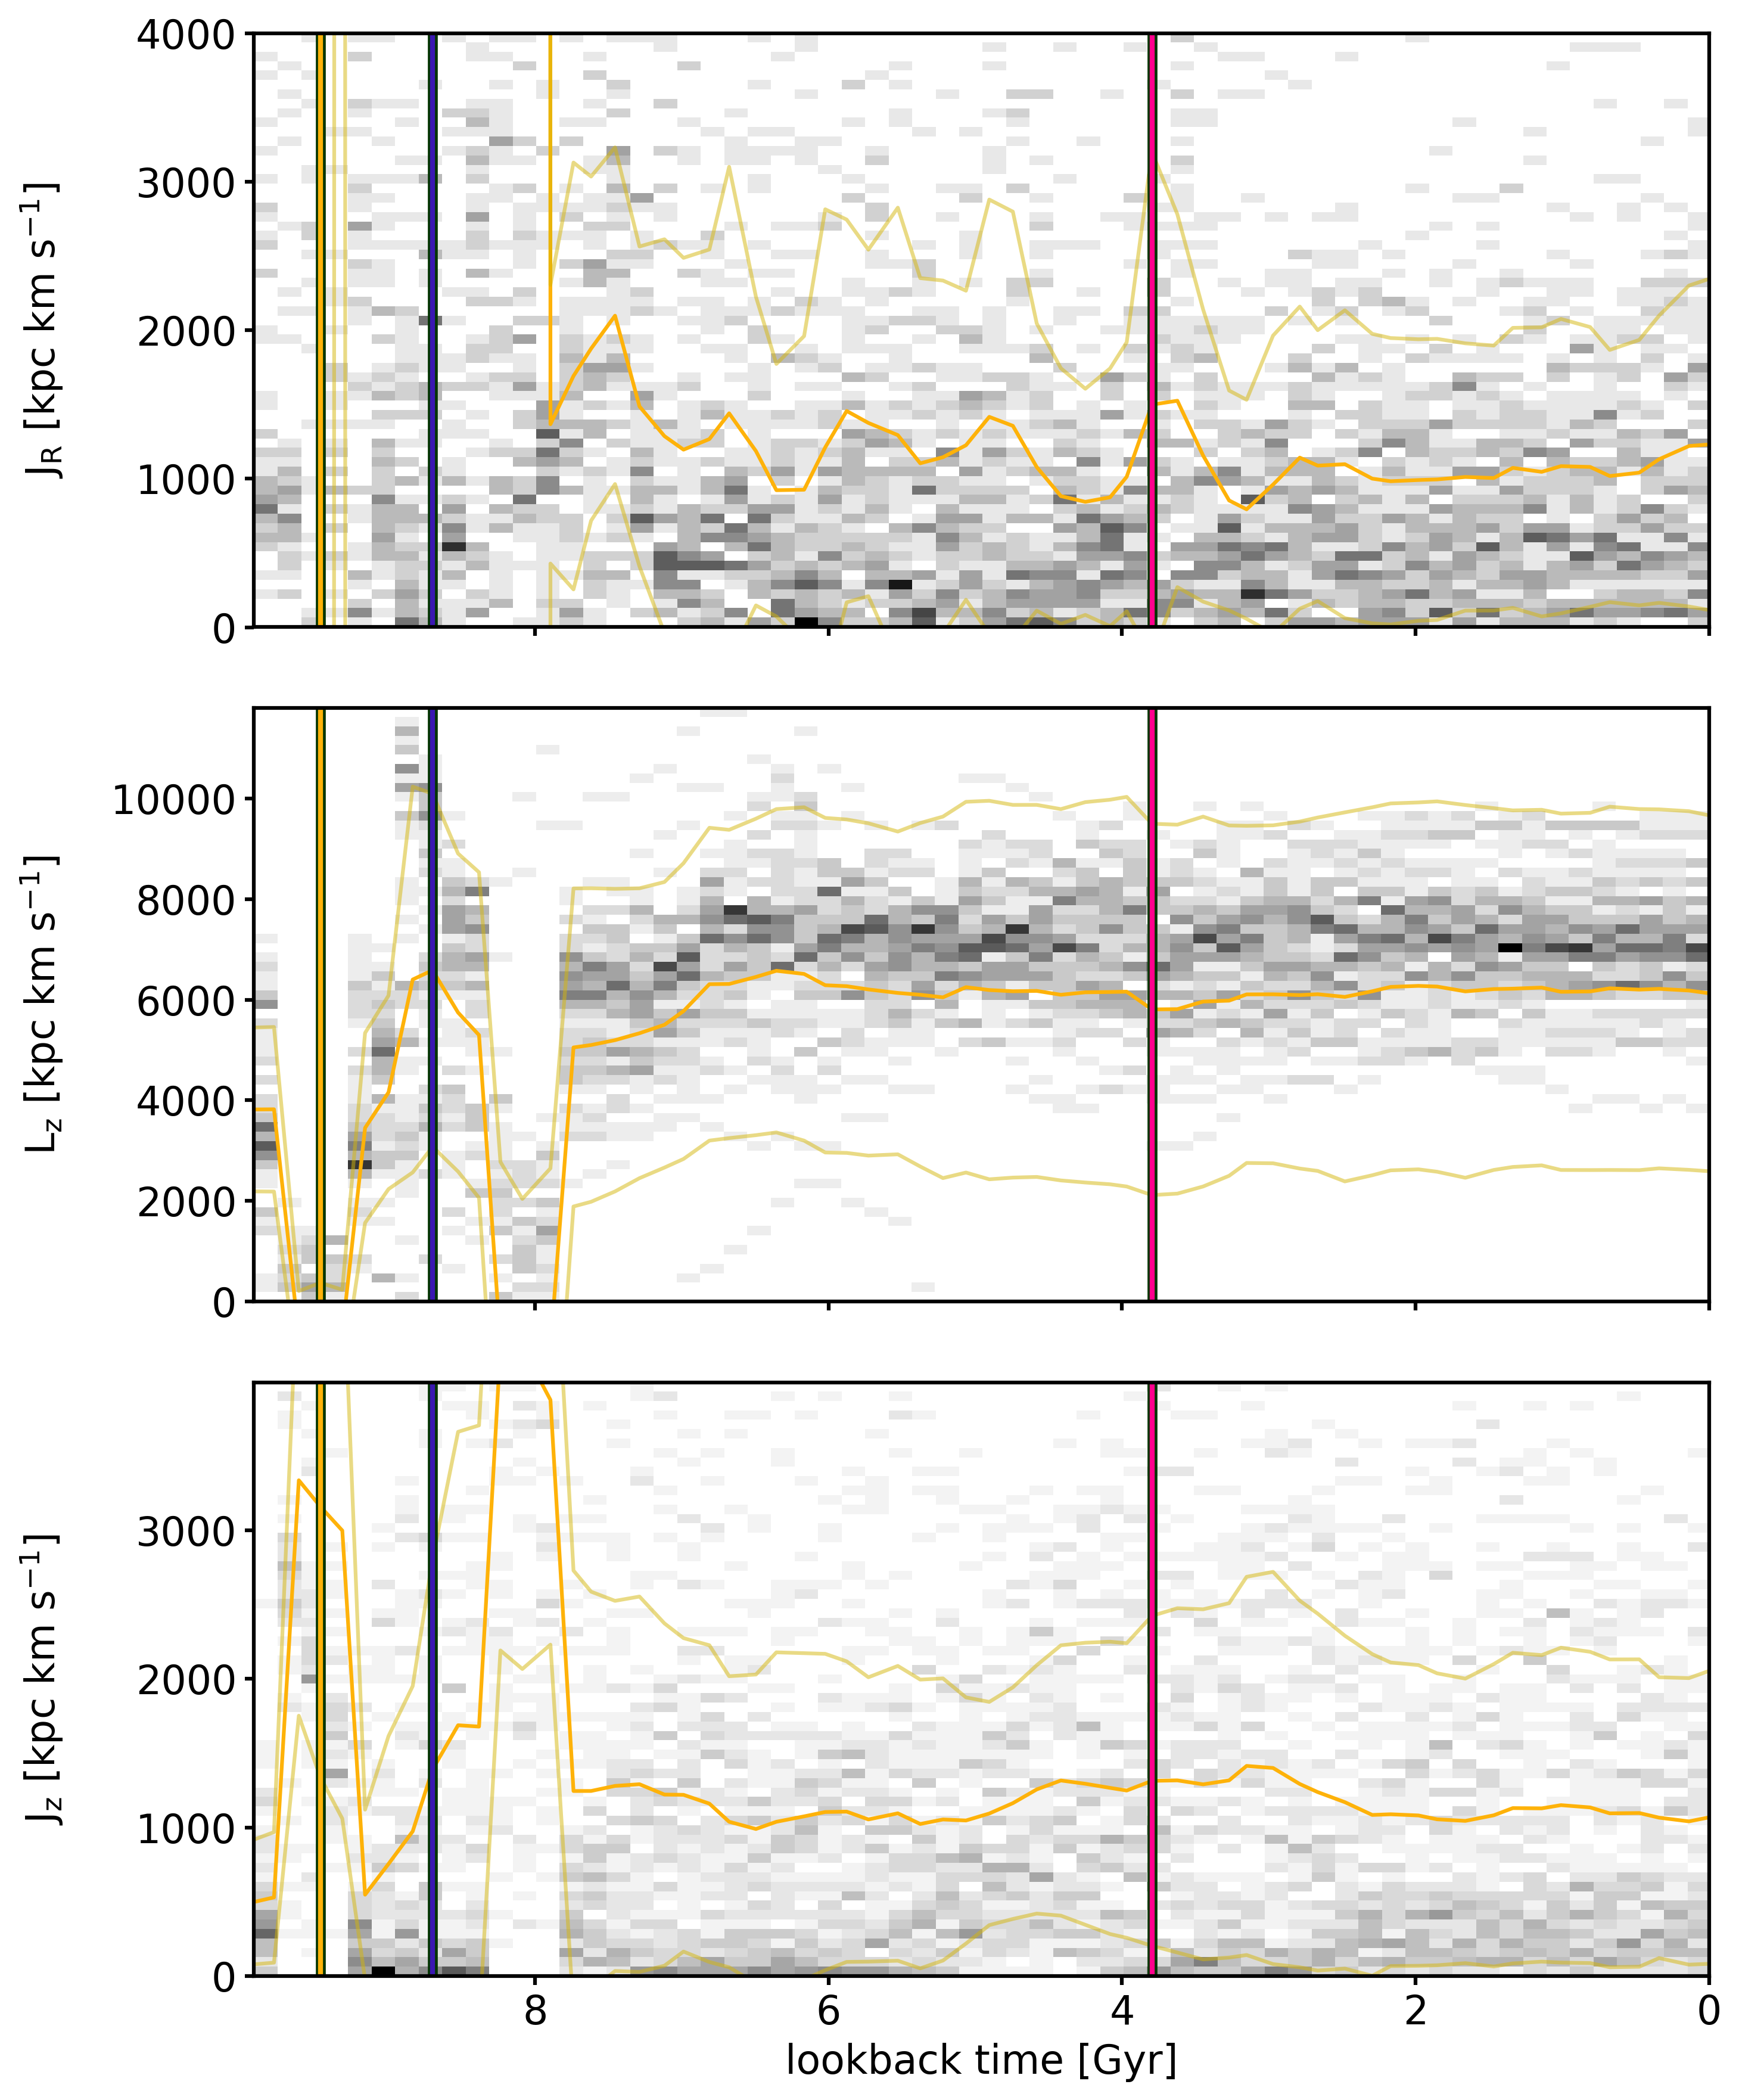
\includegraphics[width=\textwidth]{plots/Dynamics/prog4/action_time_evolution_hist_mean.png}
    \caption{Same as in Figure \ref{fig:actions_time_evolution_prog2}, only for prog4. Now the pink, blue and yellow lines indicate times of the mergers of prog2, prog3 and prog4, respectively.  }\label{fig:actions_time_evolution_prog4}
\end{figure}

\subsubsection{Mean best fit potential}\label{subsubsec:GCs_actions_time_mean_right_pot}

\begin{figure}[htbp]
\captionsetup{format=plain}
    \centering
	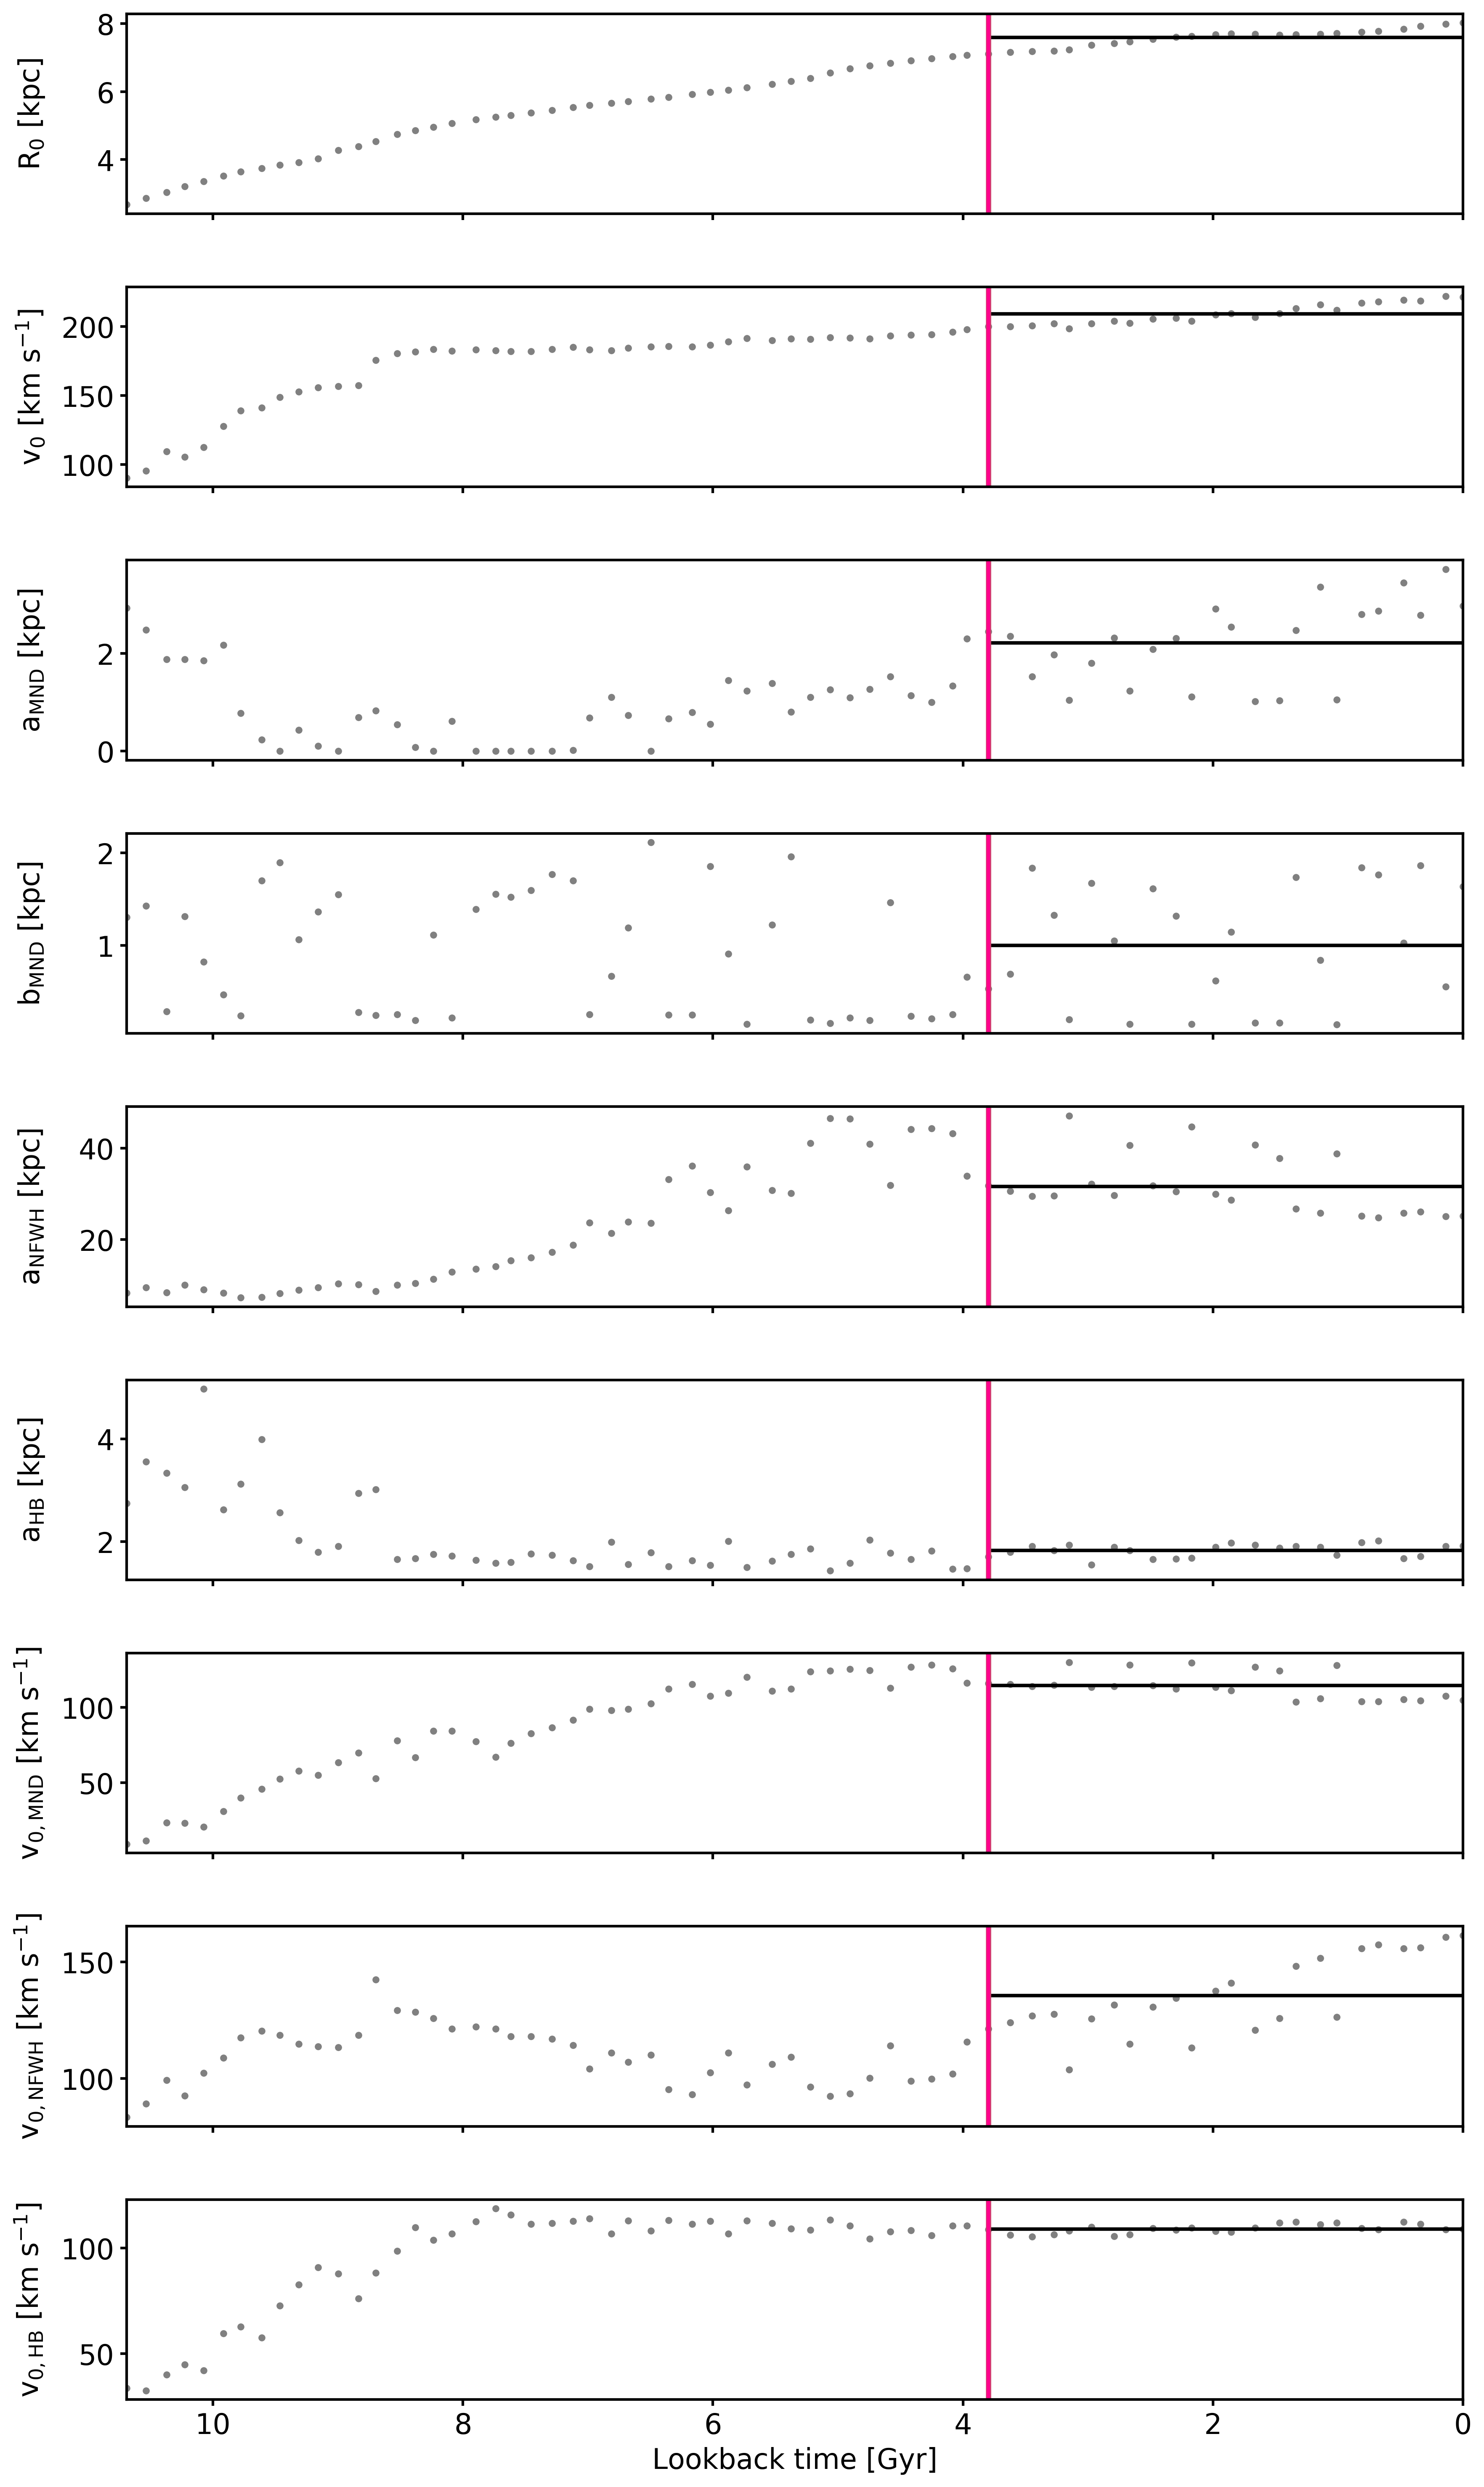
\includegraphics[width=0.8\textwidth]{plots/Dynamics/mean_pot/potential_evolution_with_mean_dec18.png}
    \caption{Time evolution of best fit potential parameters and their mean values since the merger of prog2 (indicated in pink).}\label{fig:potential_mean_evolution}
\end{figure}

\begin{figure}[htbp]
\captionsetup{format=plain}
    \centering
	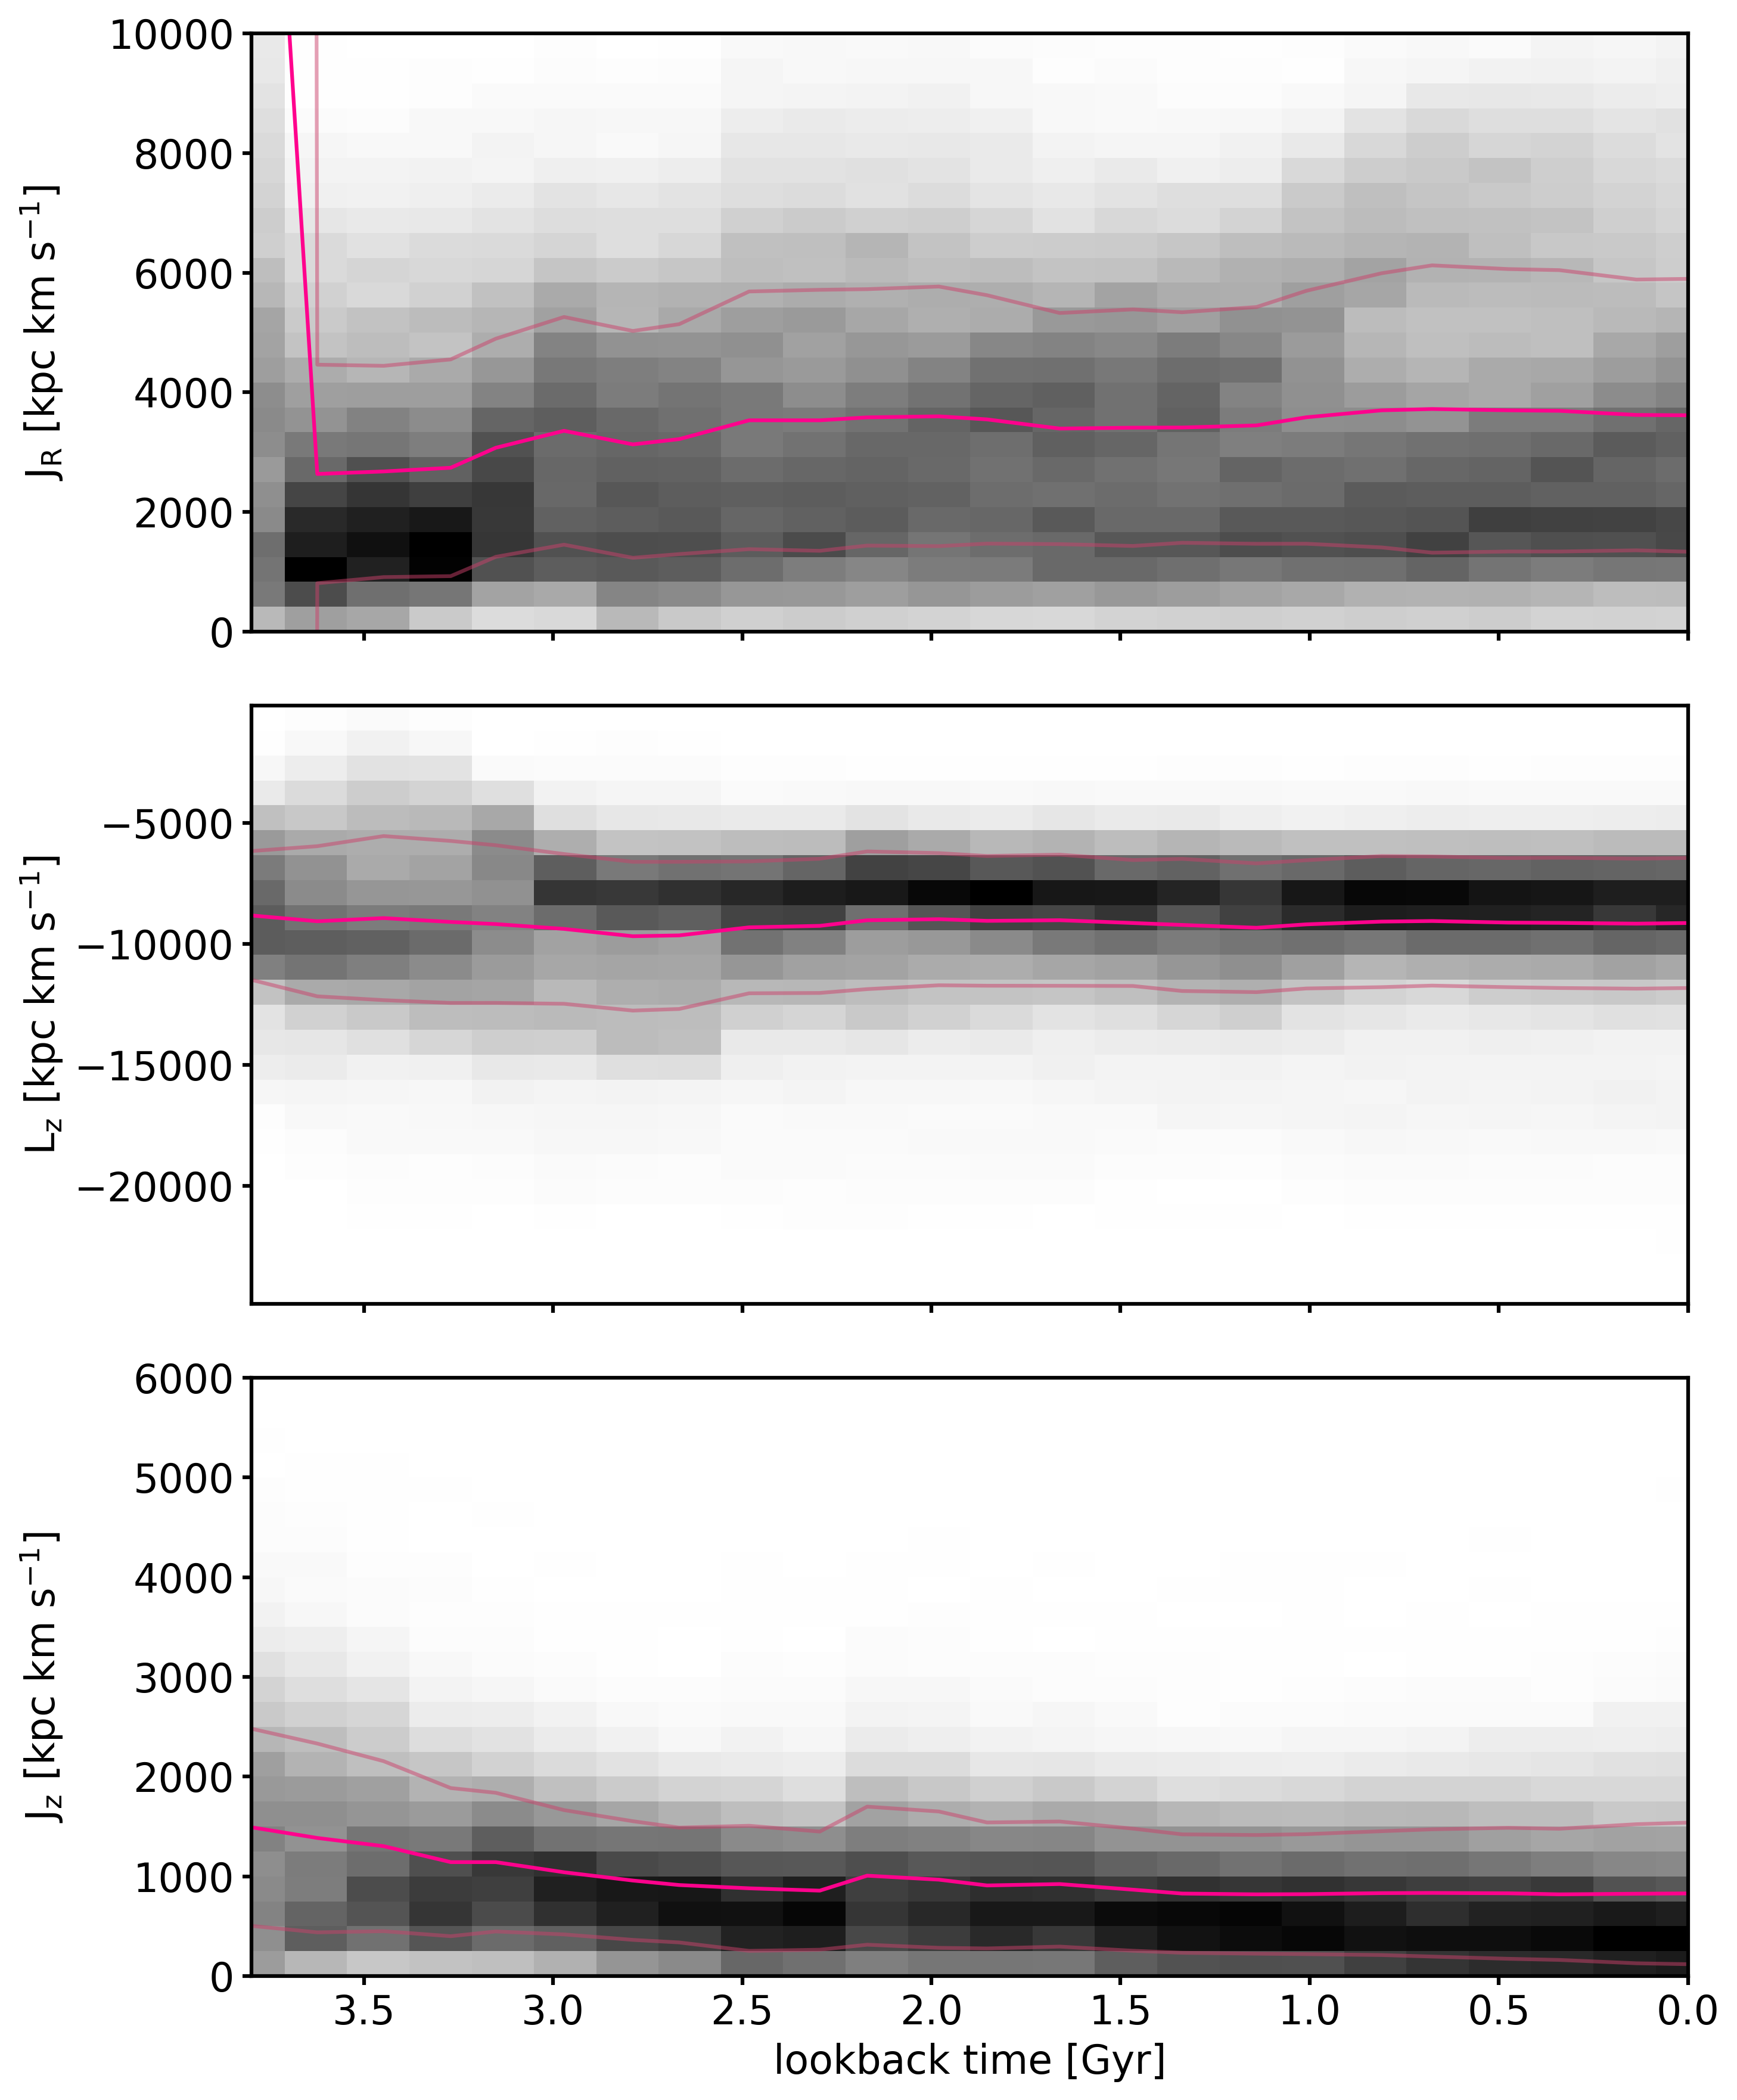
\includegraphics[width=\textwidth]{plots/Dynamics/mean_pot/action_time_evolution_hist_mean_prog2.png}

	\caption{Same as Figure \ref{fig:actions_time_evolution_prog2}, only for a constant potential since the merger of prog2.}\label{fig:actions_time_evolution_mean_pot_prog2}
\end{figure}

\begin{figure}
\captionsetup{format=plain}
    \centering
	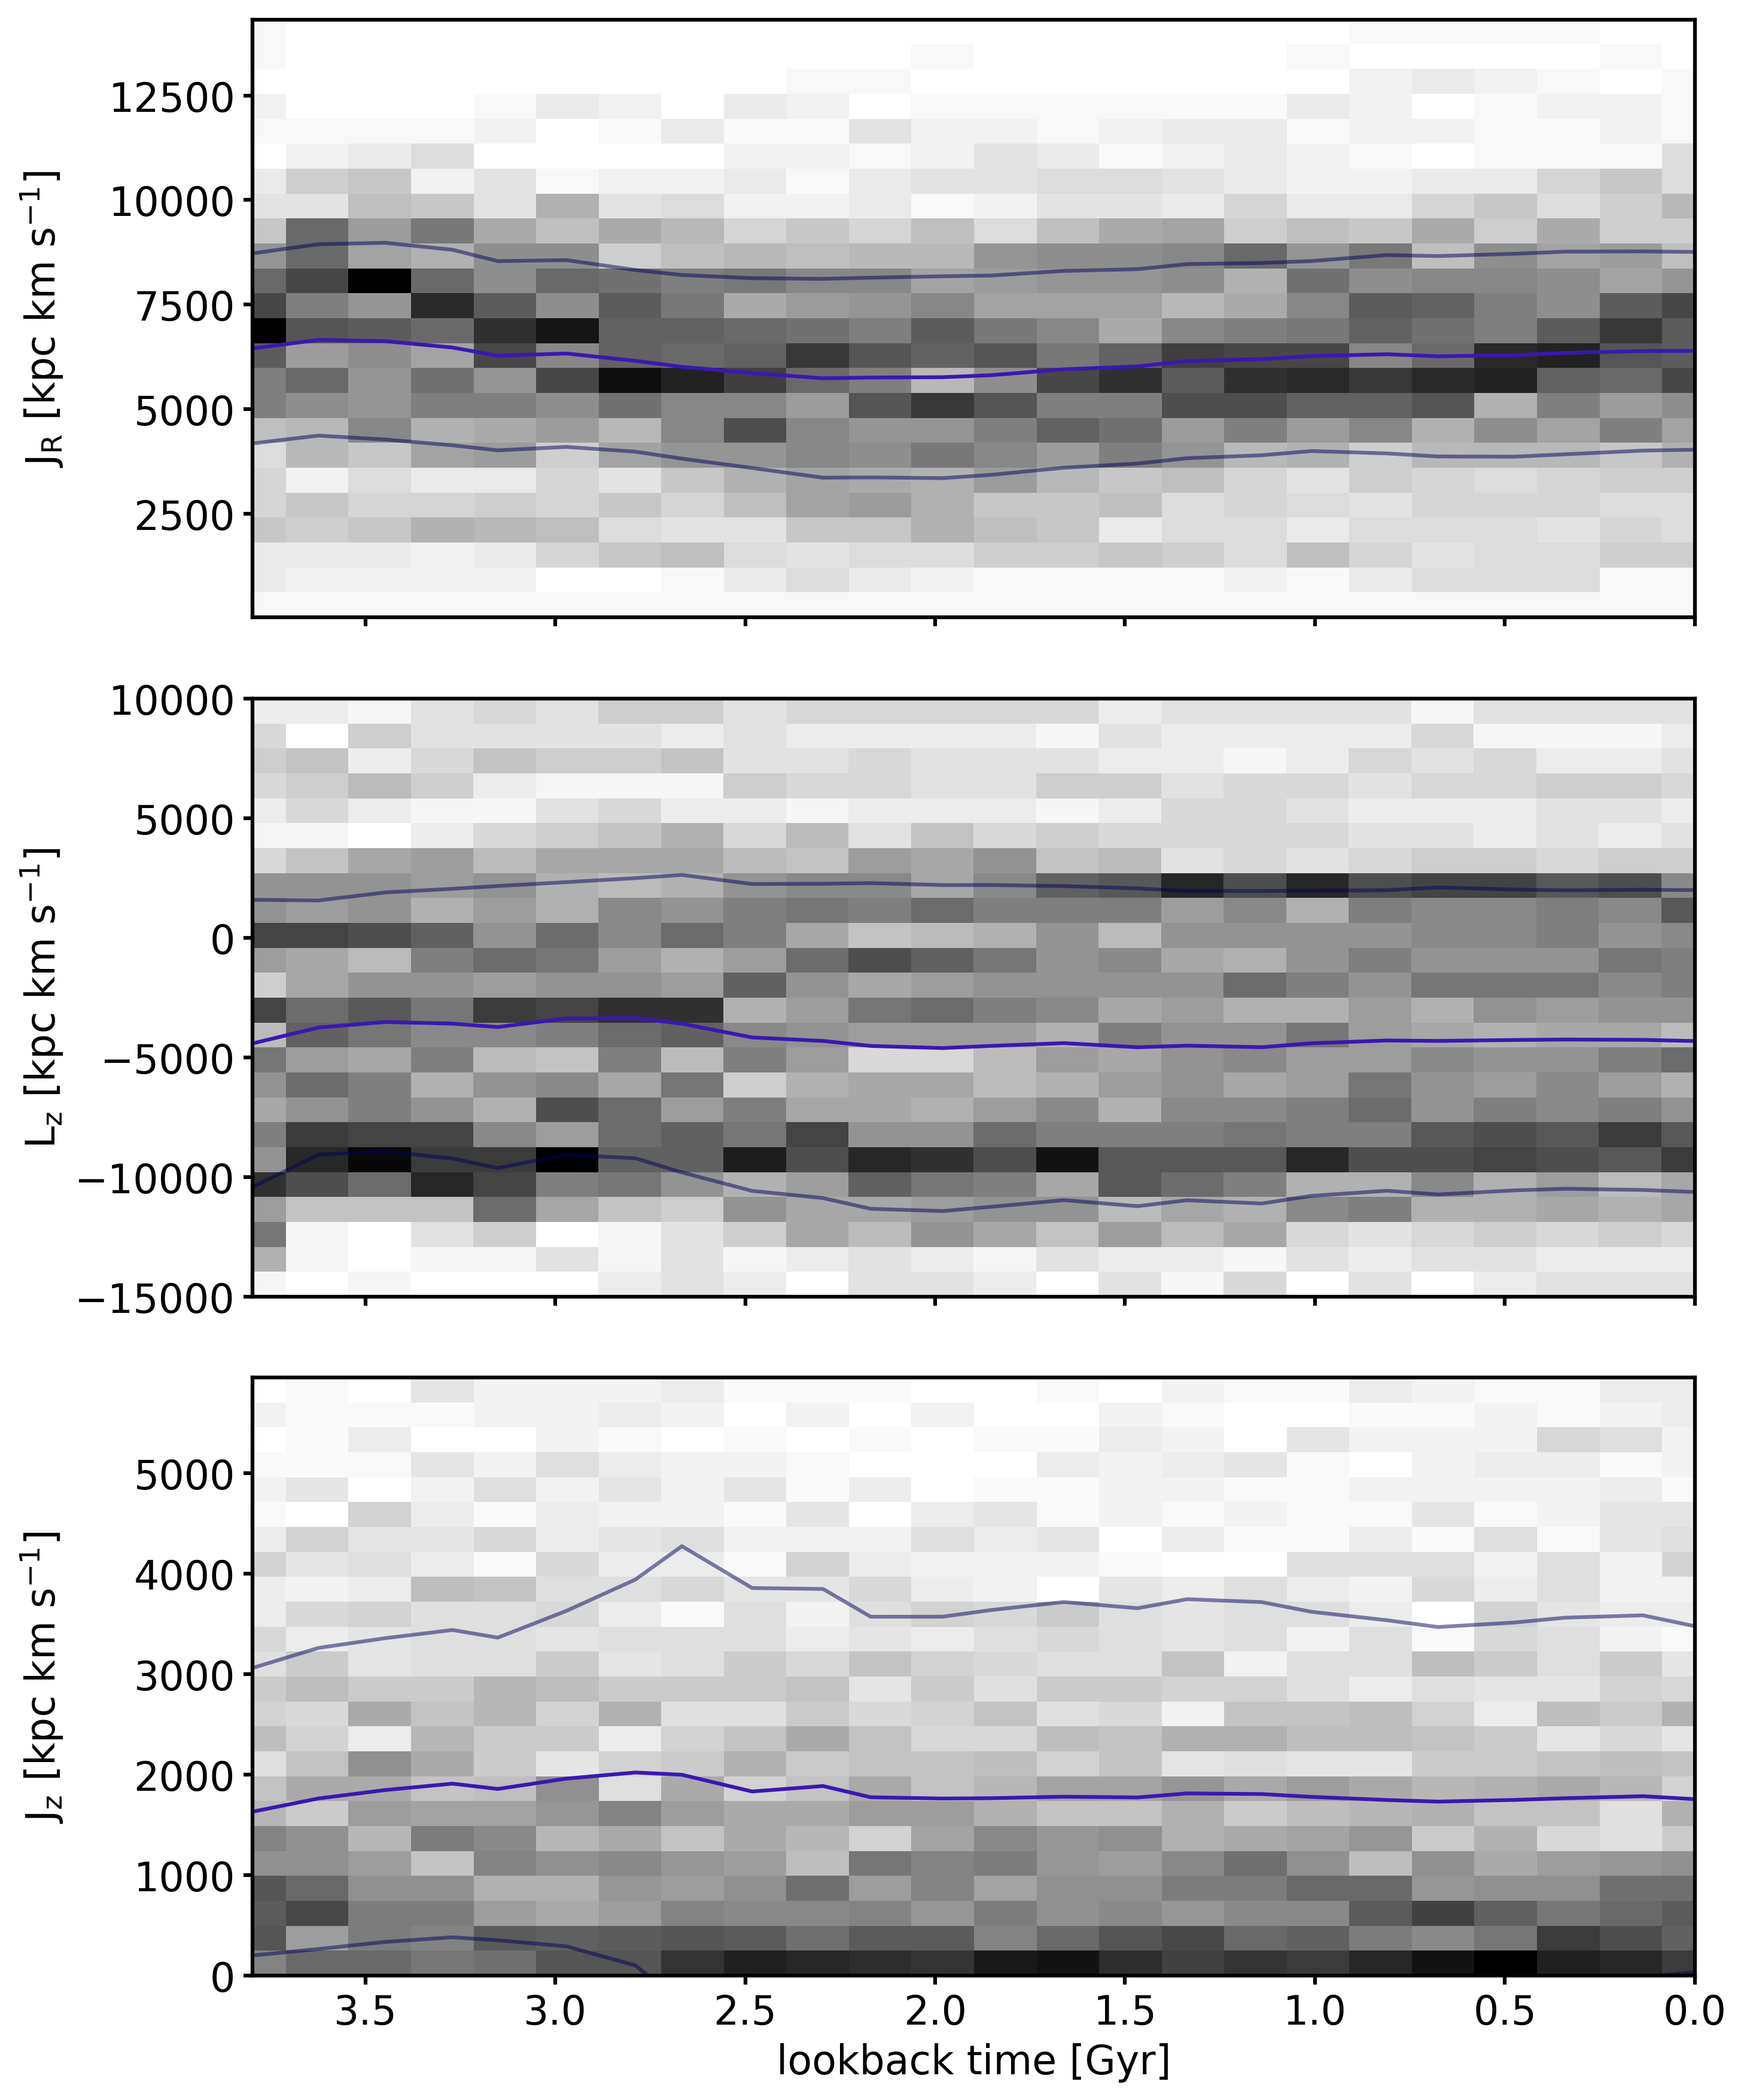
\includegraphics[width=\textwidth]{plots/Dynamics/mean_pot/action_time_evolution_hist_mean_prog3.png}
    \caption{Same as Figure \ref{fig:actions_time_evolution_prog3}, only for a constant potential since the merger of prog2.}\label{fig:actions_time_evolution_mean_pot_prog3}
\end{figure}

\begin{figure}[htbp]
\captionsetup{format=plain}
    \centering
	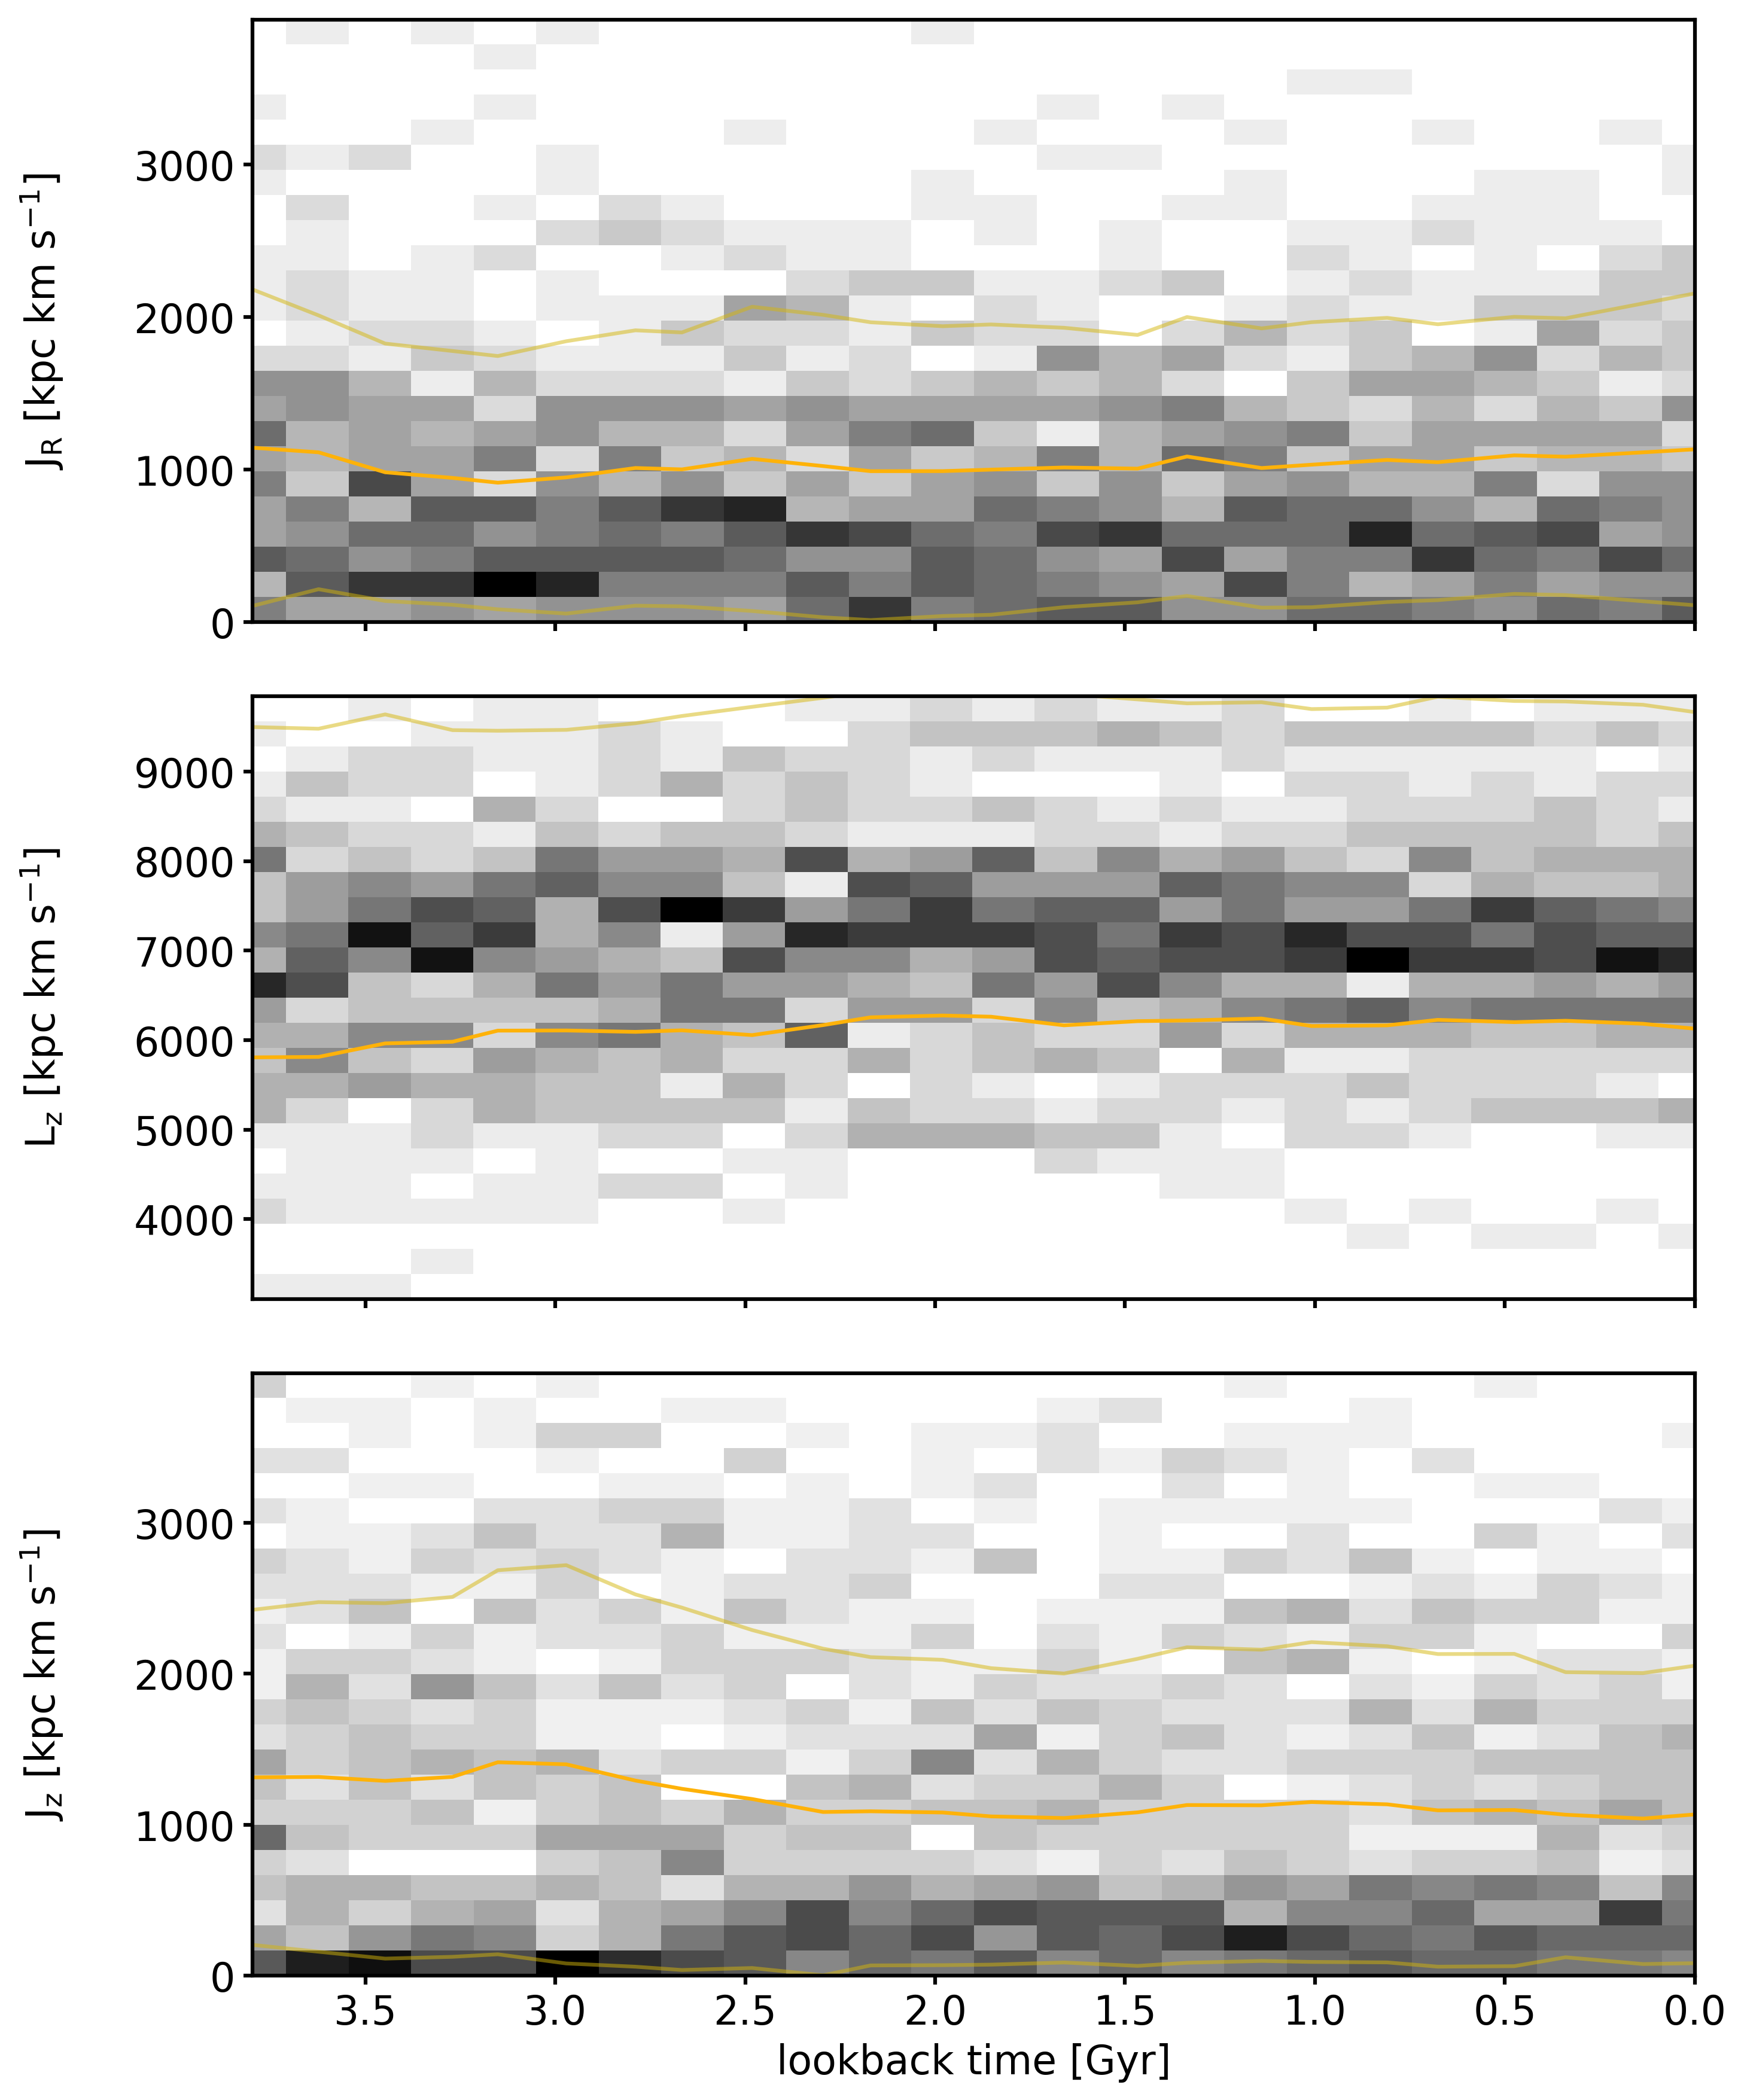
\includegraphics[width=\textwidth]{plots/Dynamics/mean_pot/action_time_evolution_hist_mean_prog4.png}
    \caption{Same as Figure \ref{fig:actions_time_evolution_prog4}, only for a constant potential since the merger of prog2.}\label{fig:actions_time_evolution_mean_pot_prog4}
\end{figure}

\subsubsection{Energy evolution}\label{subsubsec:energy_evol}
\begin{figure}[htbp]
\captionsetup{format=plain}
    \centering
	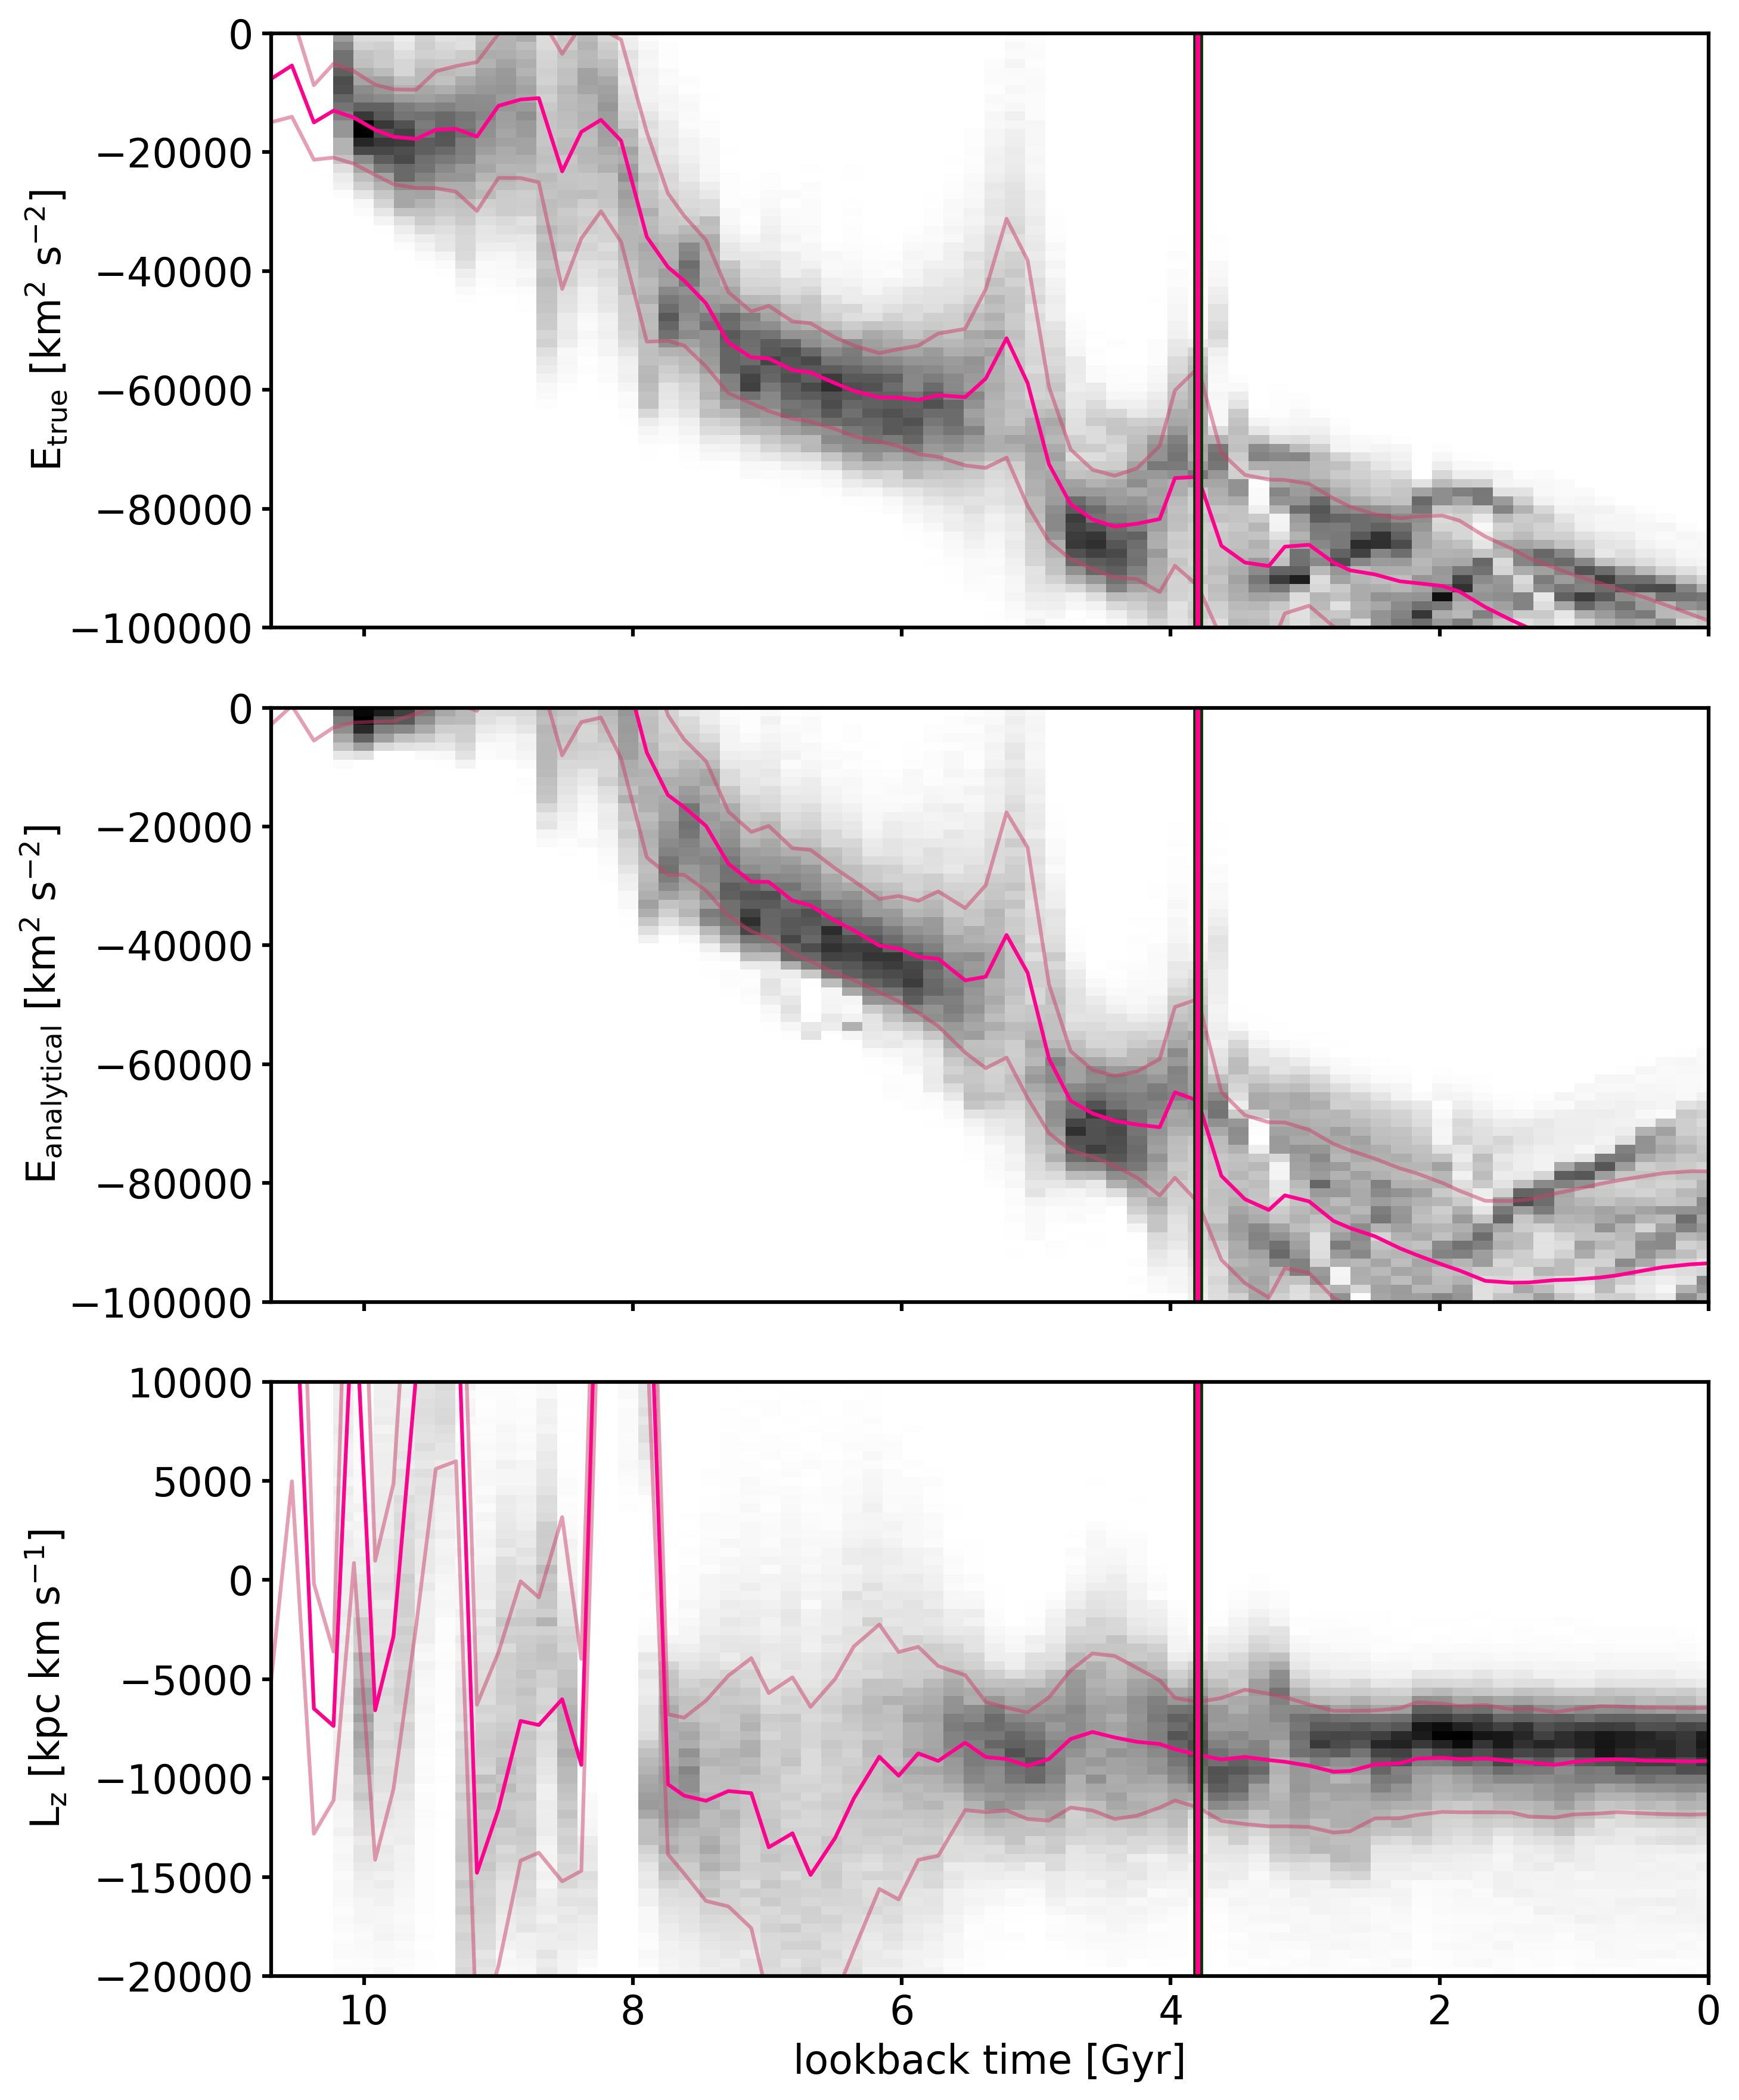
\includegraphics[width=\textwidth]{plots/Dynamics/prog2/energy_time_evolution_hist_mean.png}
	\caption{Time evolution of the energy of the particles of prog2. \textit{Upper panel}: The true energy, which the particles have according to their kinetic energy and their 'pot' value. \textit{Middle panel}: Energy calculated in the best fit potential. \textit{Lower panel}: Angular momentum.}\label{fig:energy_time_evolution_prog2}
\end{figure}

\begin{figure}
\captionsetup{format=plain}
    \centering
	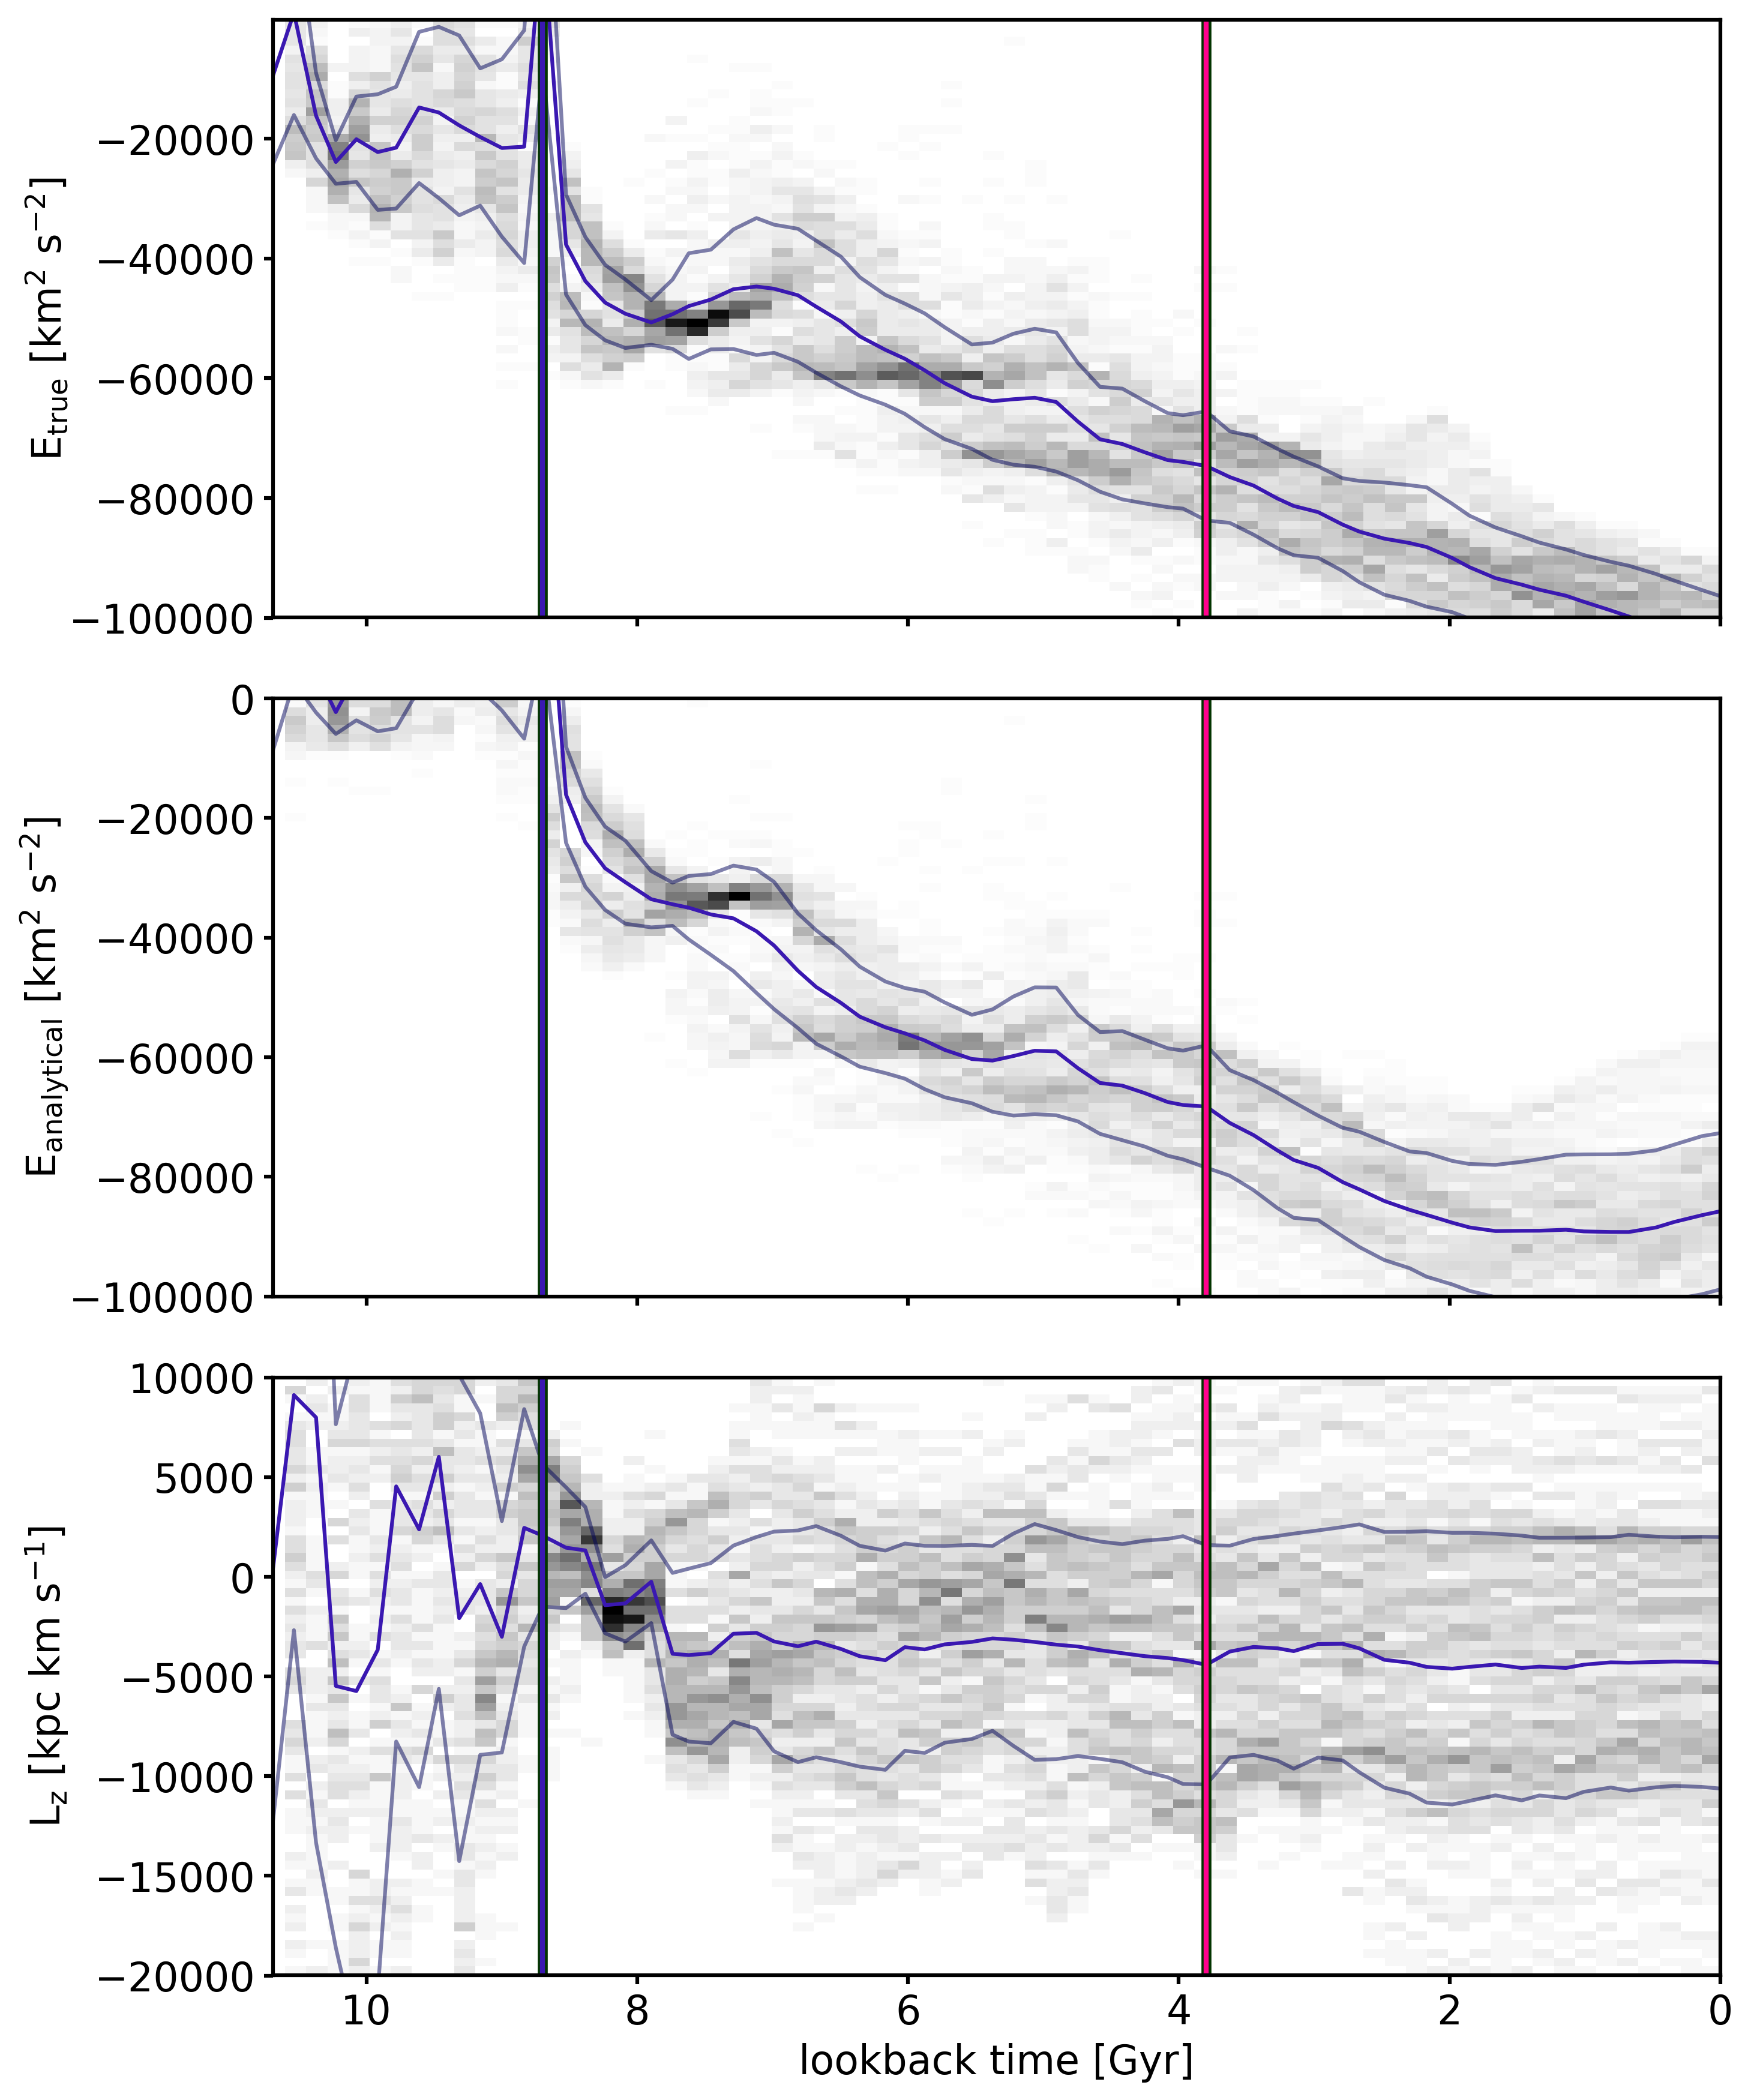
\includegraphics[width=\textwidth]{plots/Dynamics/prog3/energy_time_evolution_hist_mean.png}
    \caption{Same as \ref{fig:energy_time_evolution_prog2} but for prog3. }\label{fig:energy_time_evolution_prog3}
\end{figure}

\begin{figure}[htbp]
\captionsetup{format=plain}
    \centering
	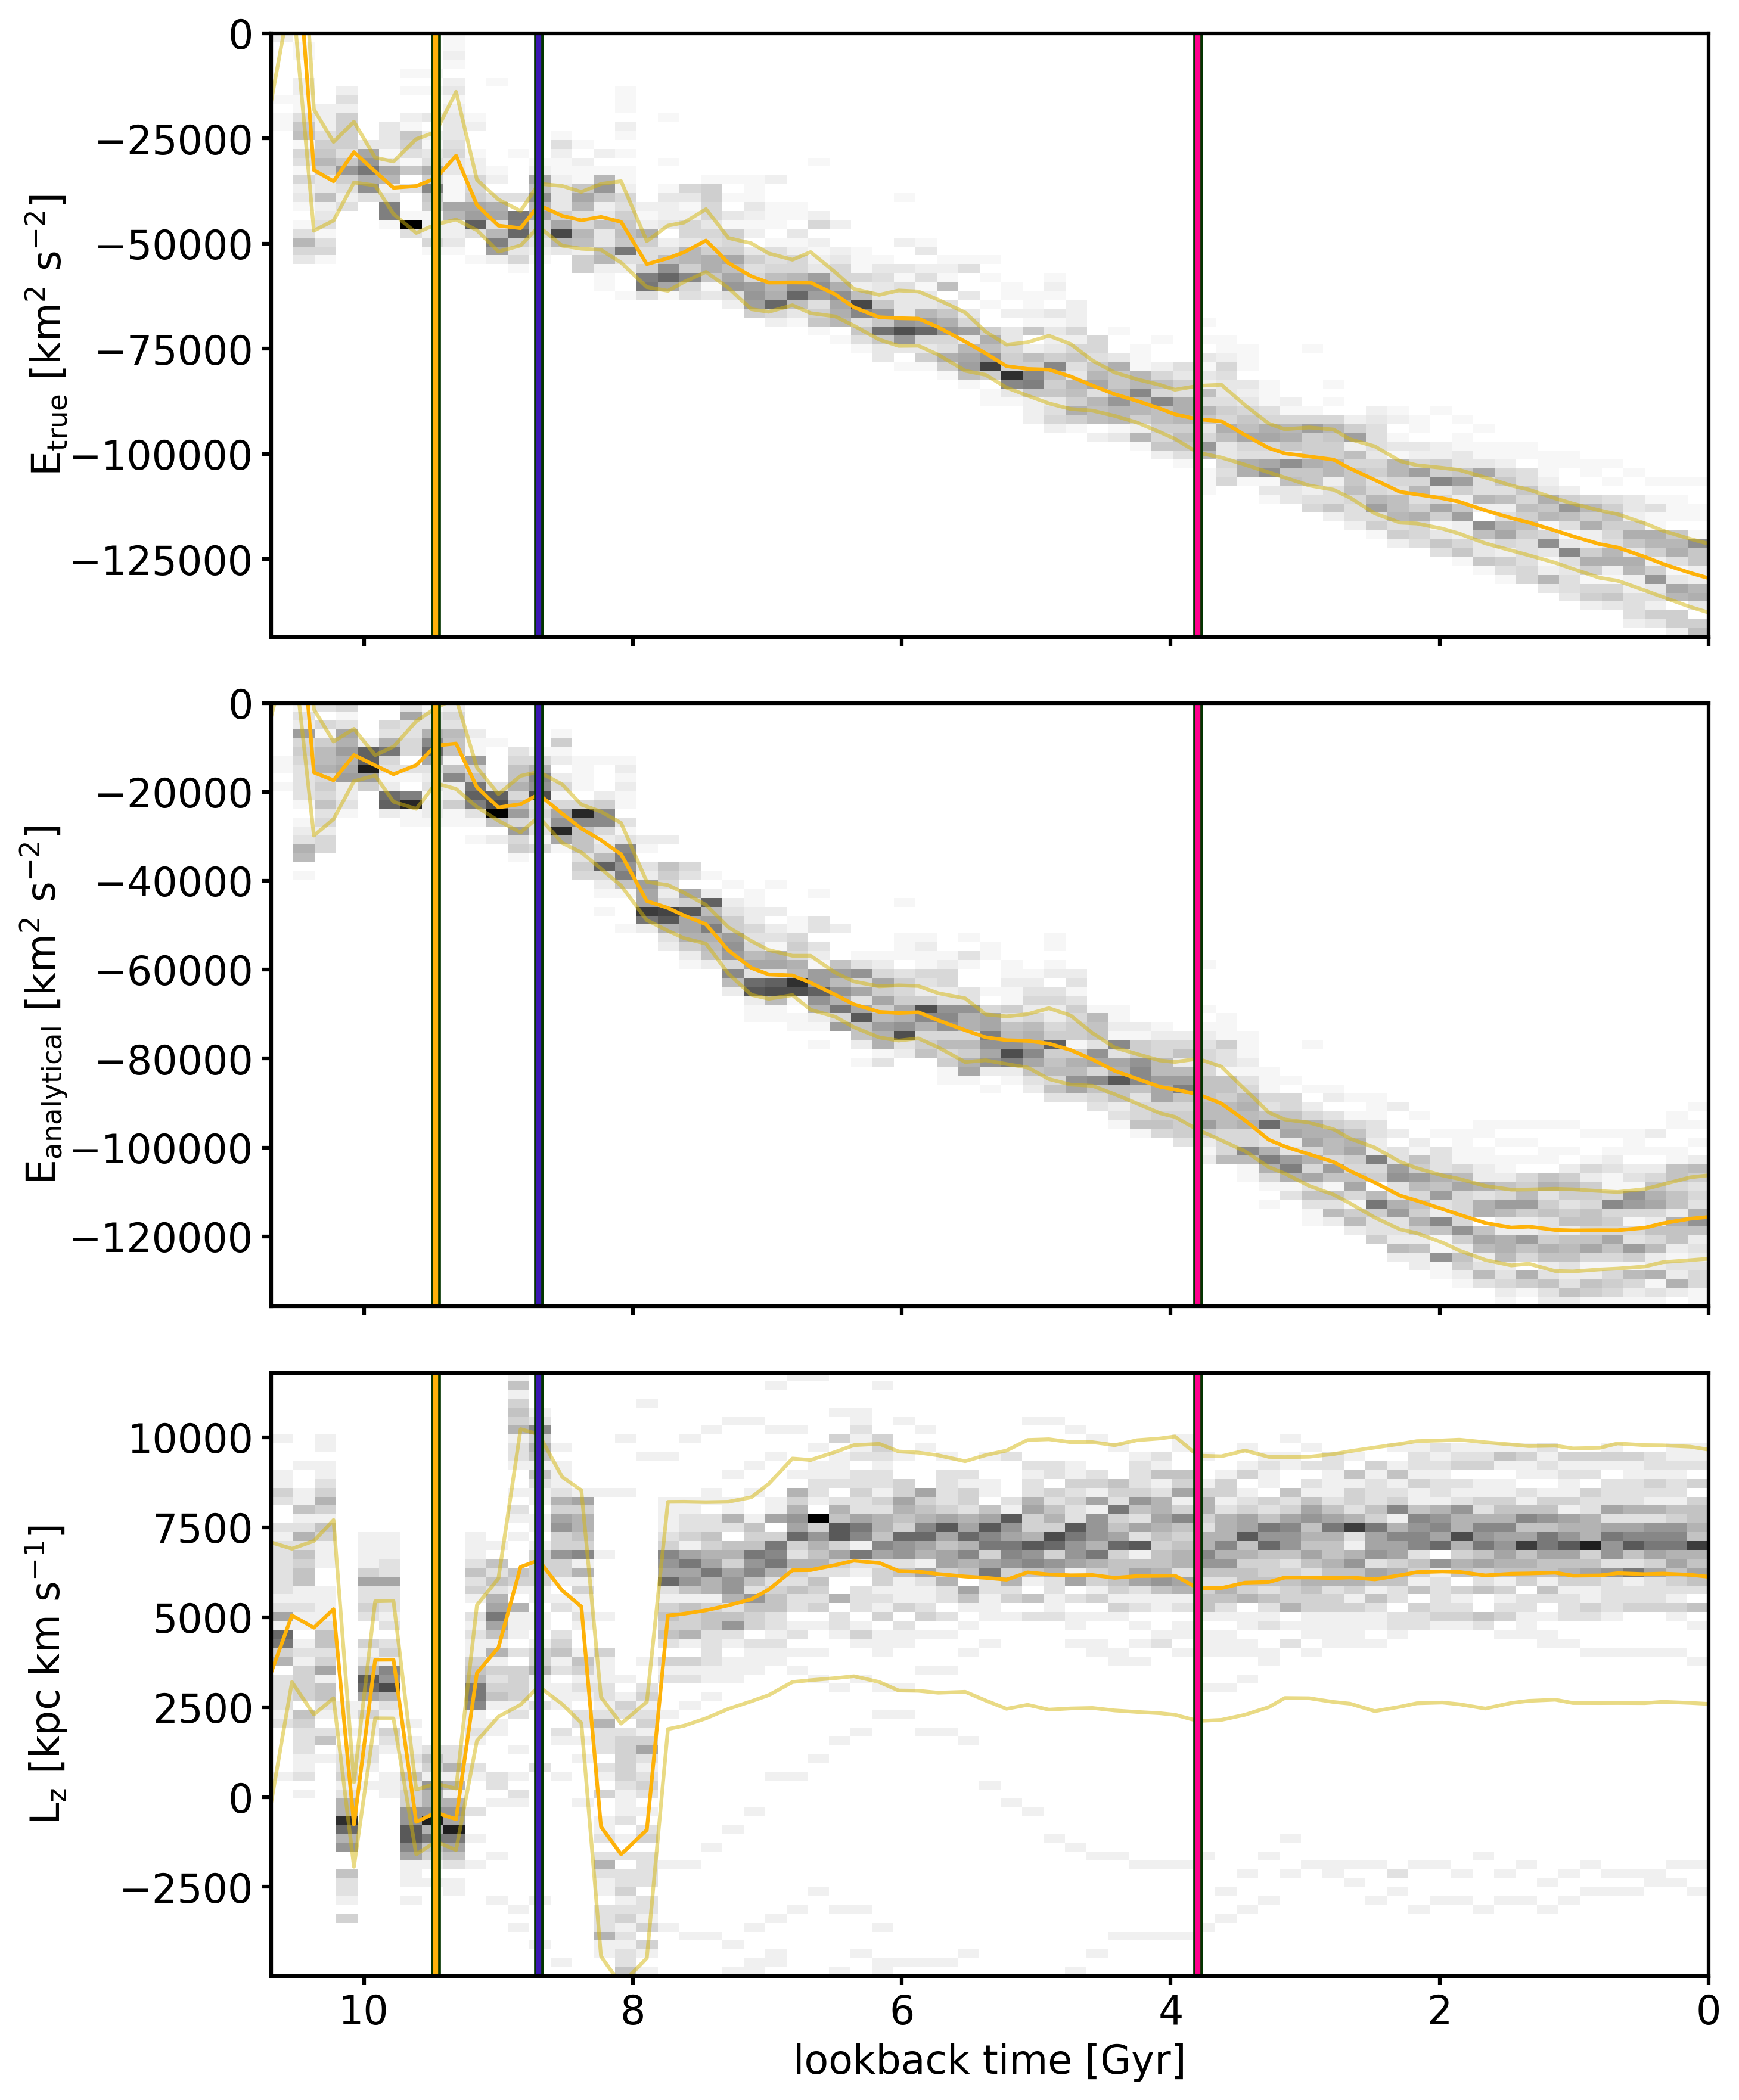
\includegraphics[width=\textwidth]{plots/Dynamics/prog4/energy_time_evolution_hist_mean.png}
    \caption{ame as \ref{fig:energy_time_evolution_prog2} but for prog4.}\label{fig:energy_time_evolution_prog4}
\end{figure}

\subsection{Test: evolution of \acp{GC} on same orbit at $z=0$}\label{subsec:box_GCs}
\begin{figure}[htbp]
\captionsetup{format=plain}
    \centering
	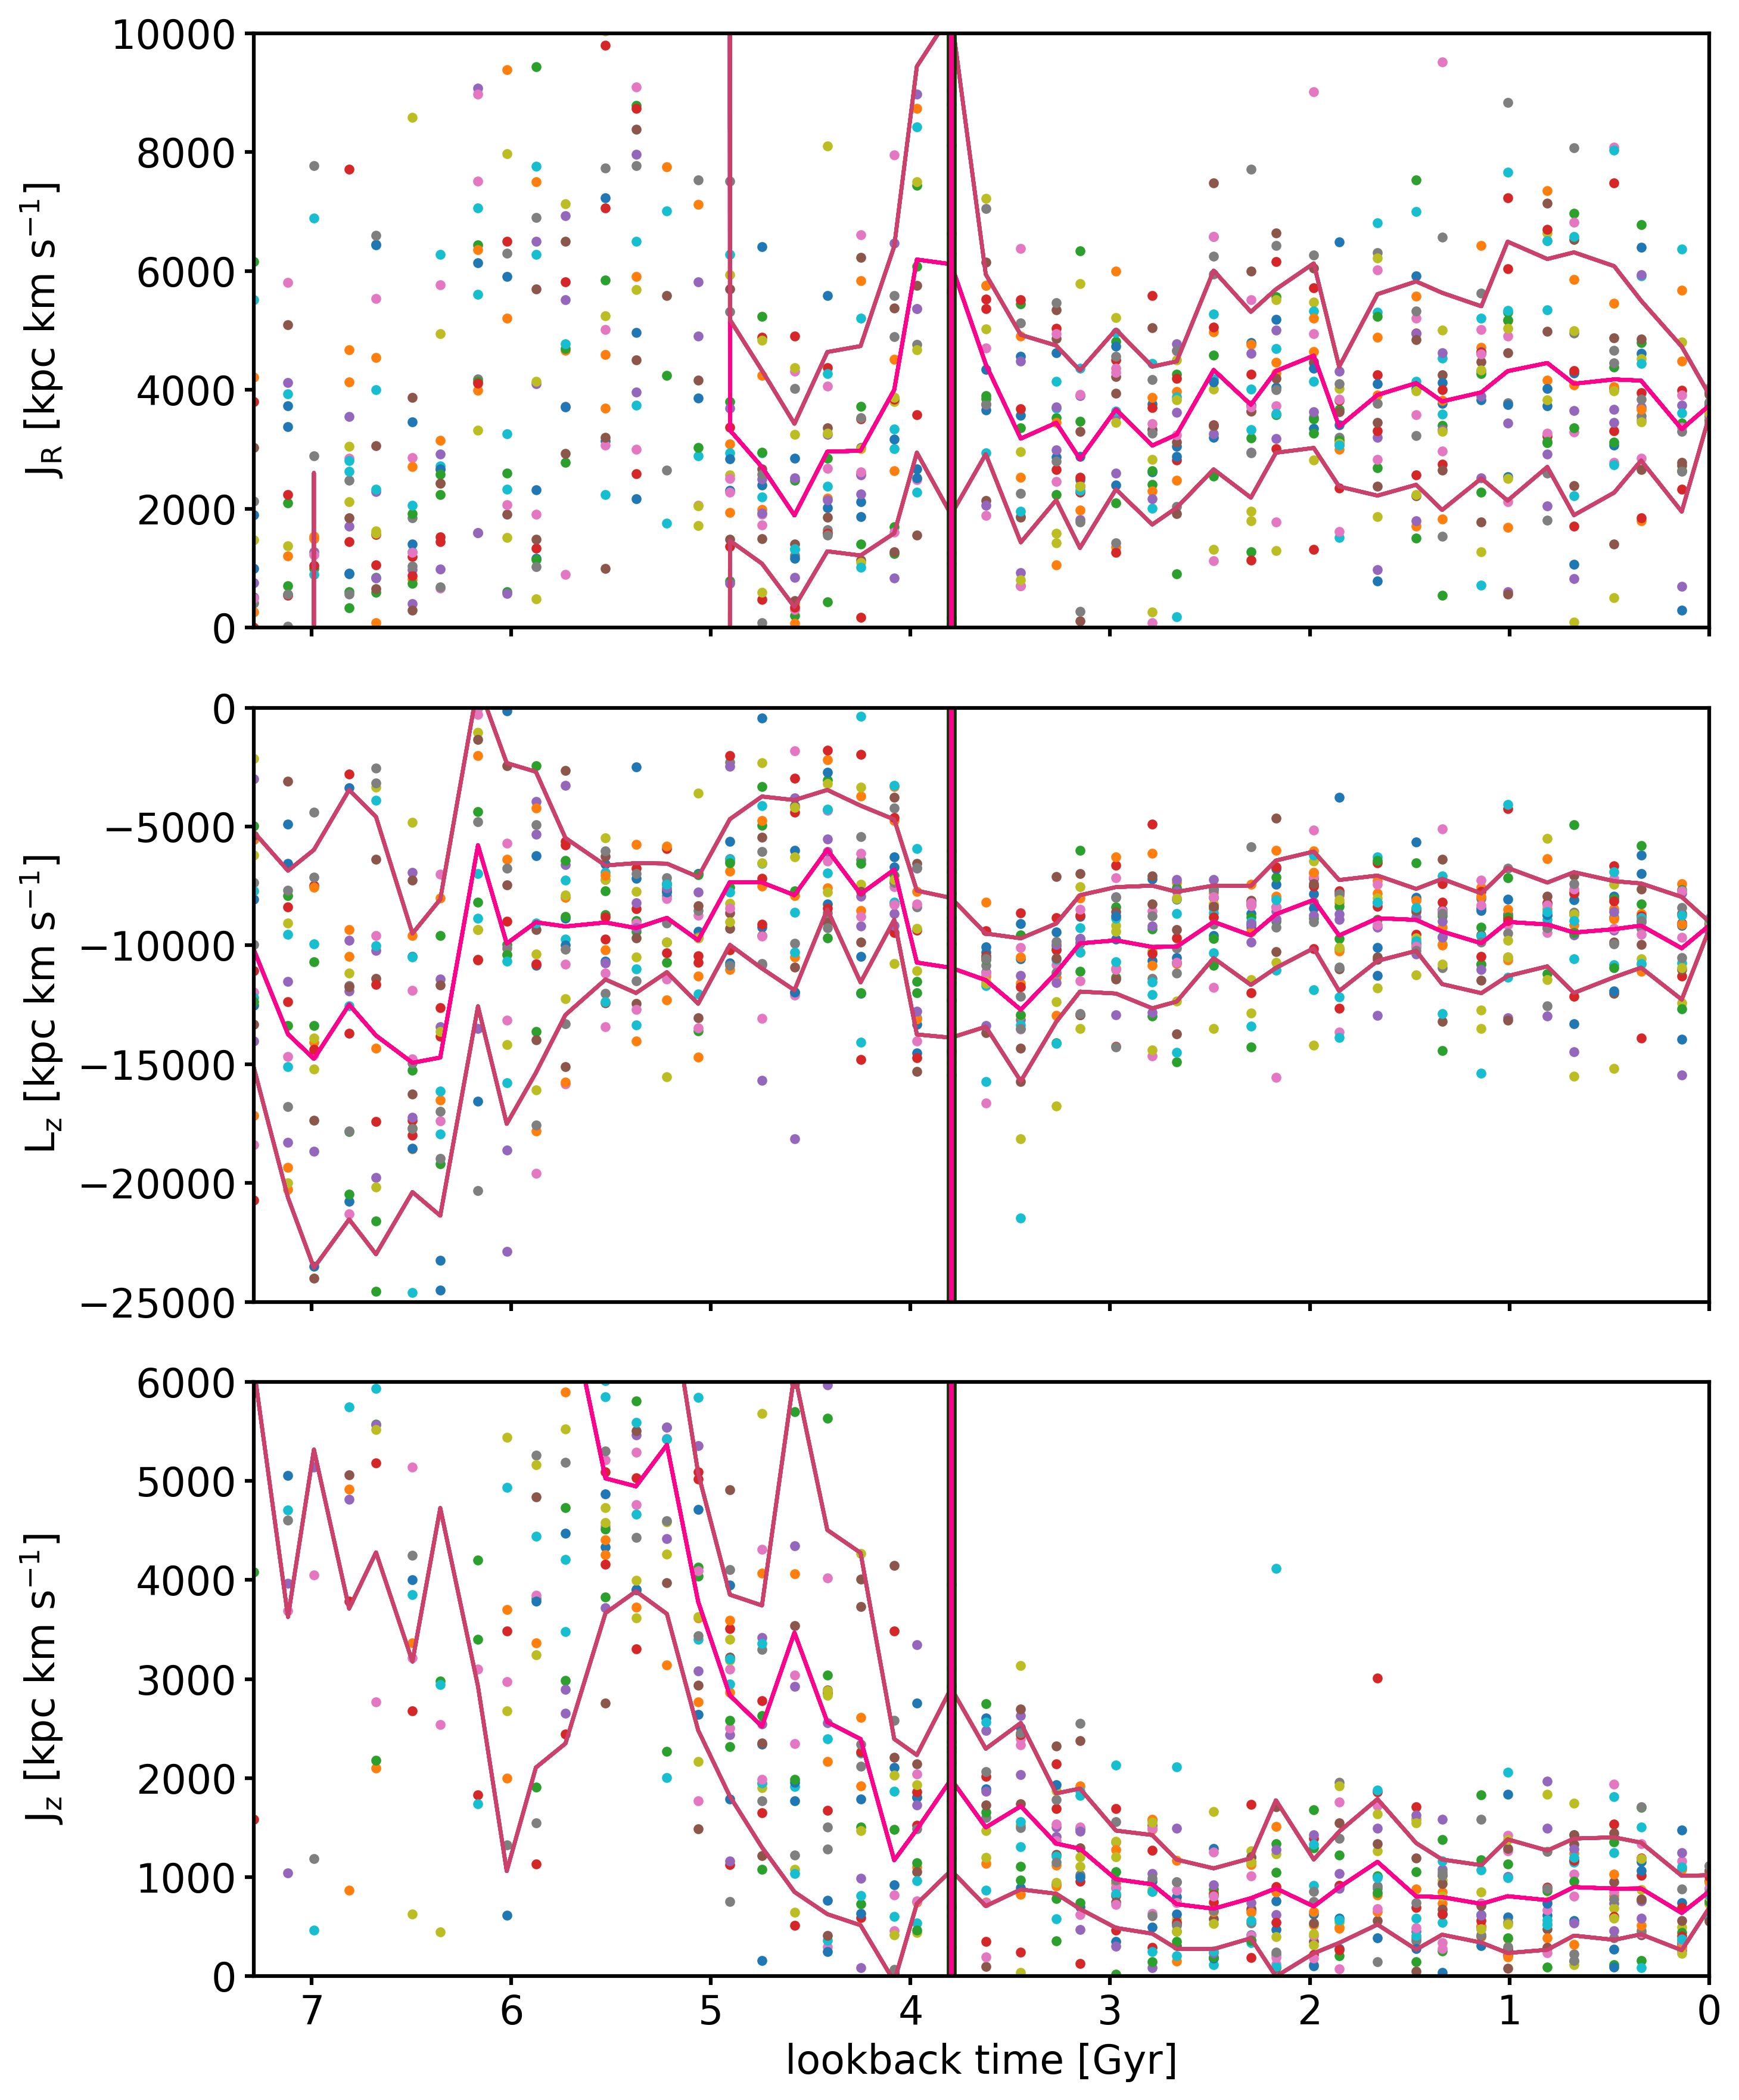
\includegraphics[width=\textwidth]{plots/Dynamics/prog2/action_time_evolution_box_hist_mean.png}

	\caption{Action time evolution of 17 particles of prog2 which are found to be on similar orbits in the $z=0$ snapshot. }\label{fig:actions_box_time_evolution_prog2}
\end{figure}

\begin{figure}
\captionsetup{format=plain}
    \centering
	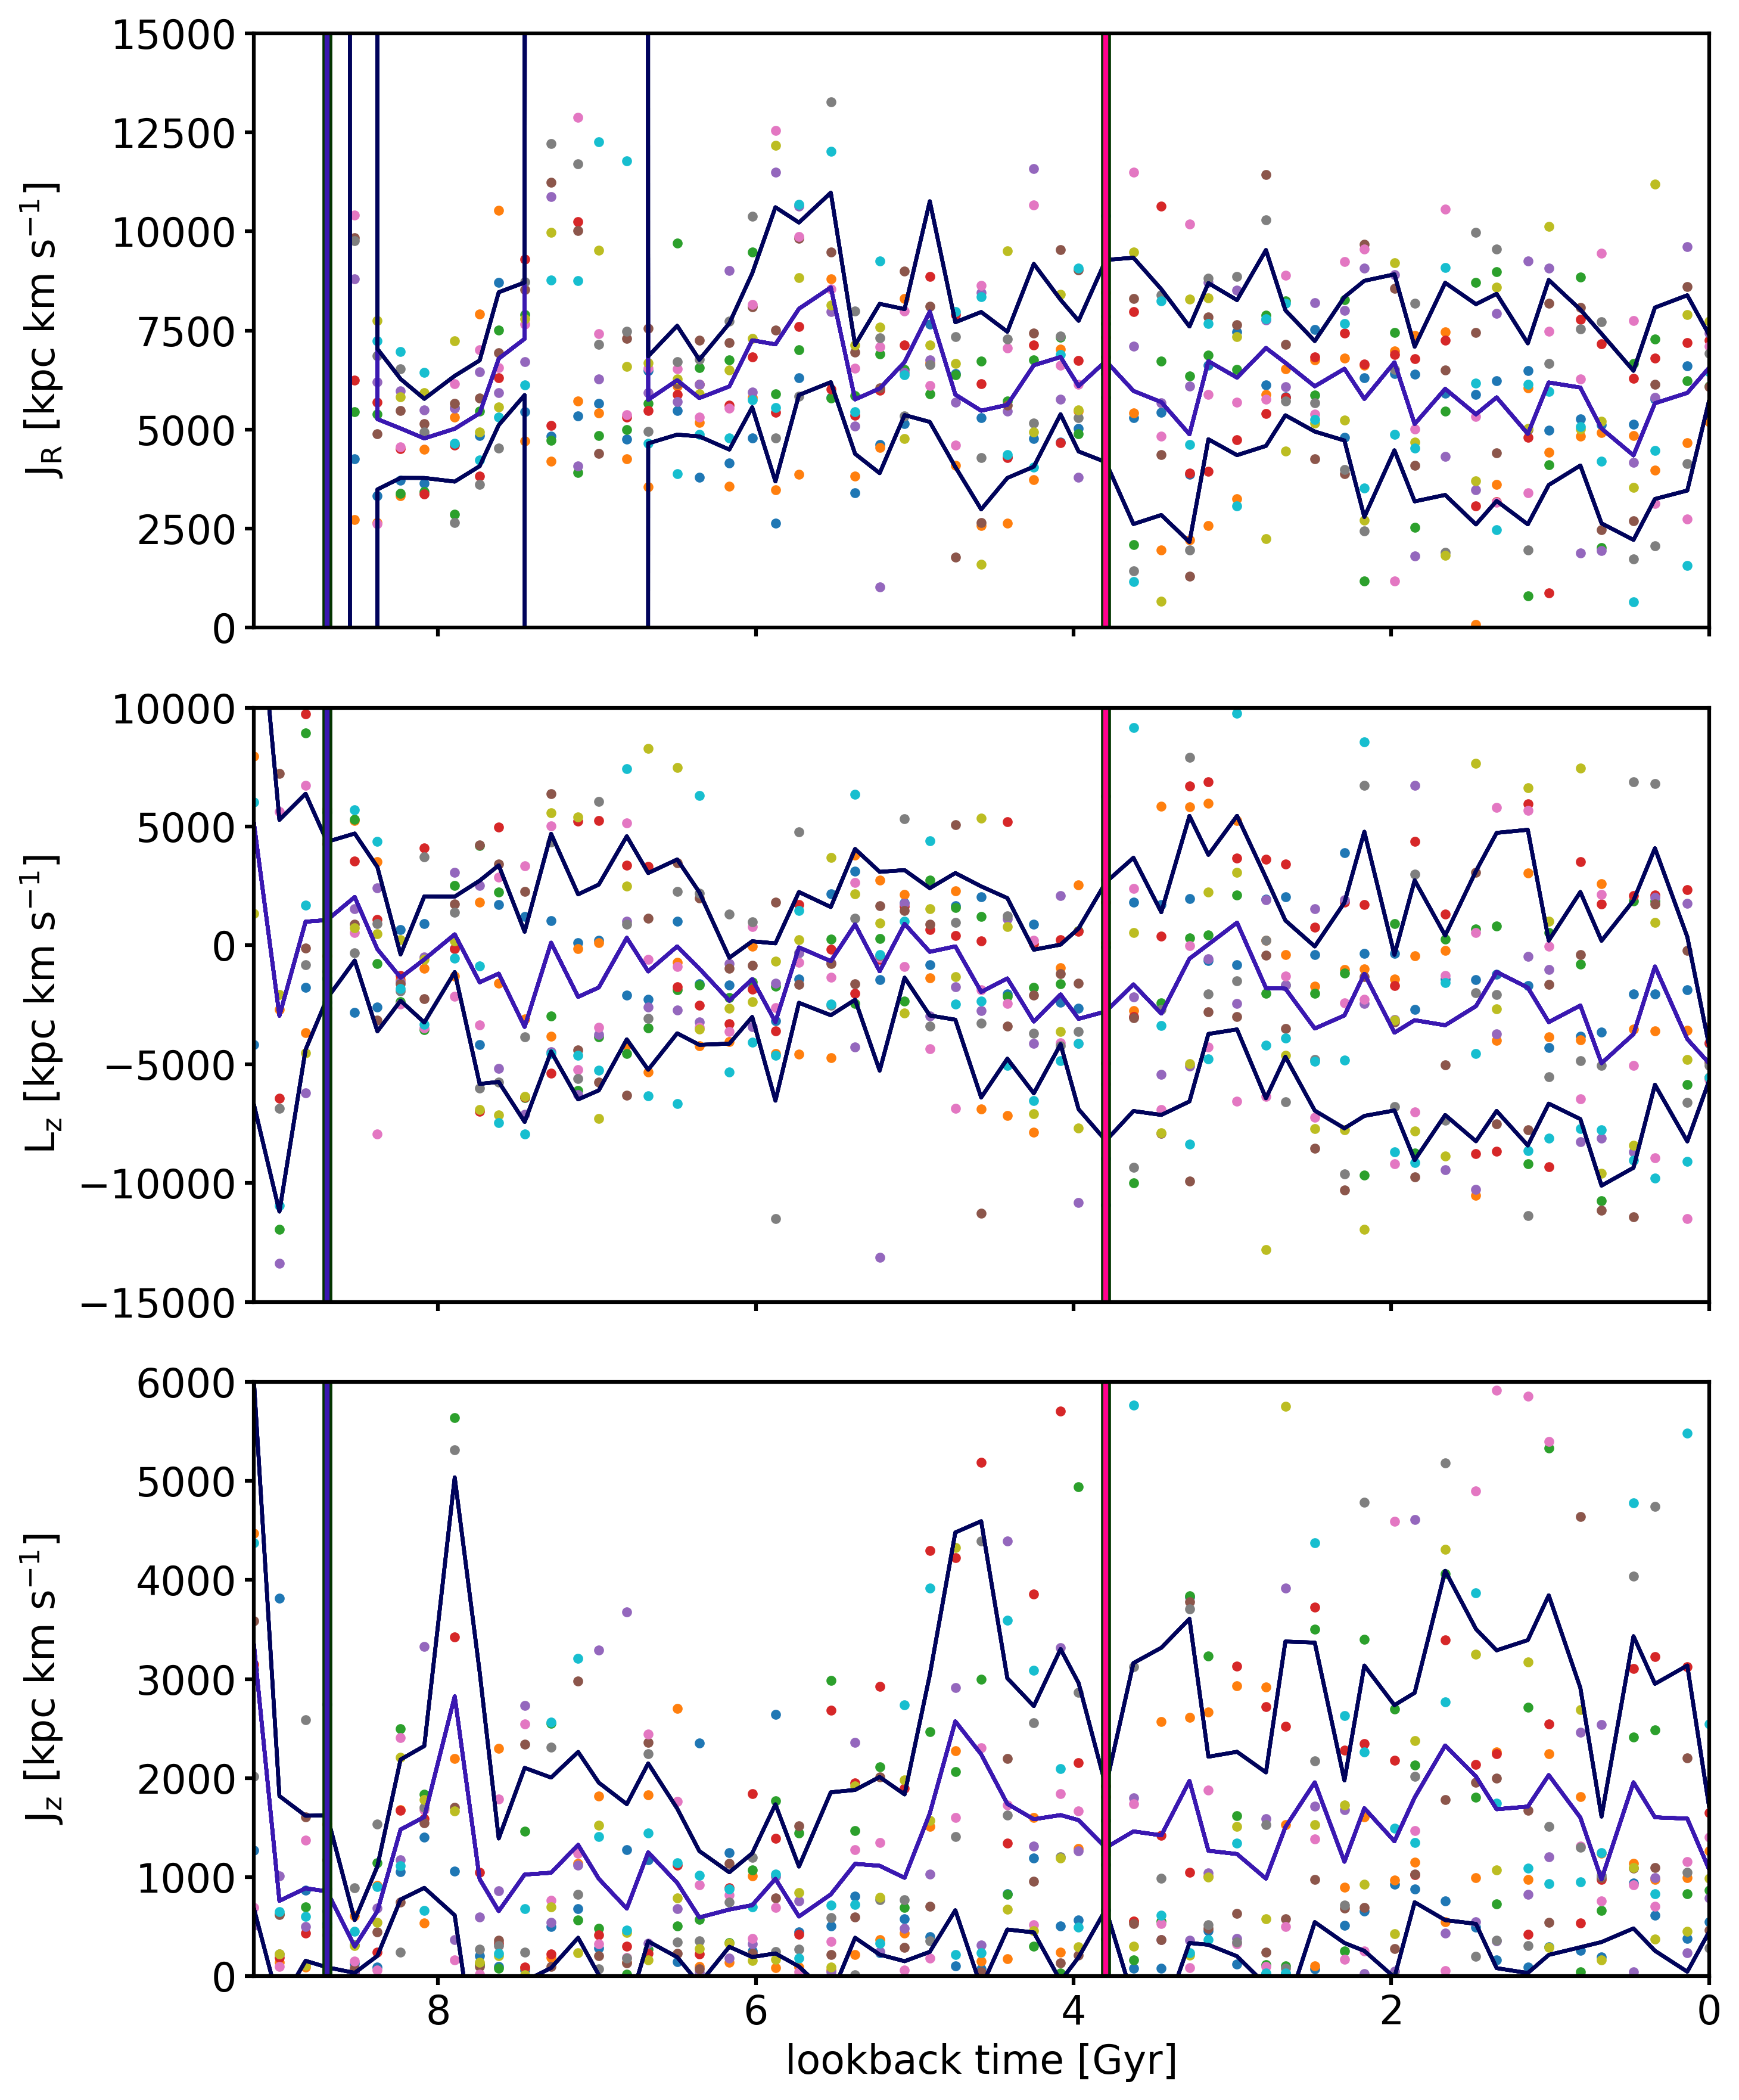
\includegraphics[width=\textwidth]{plots/Dynamics/prog3/action_time_evolution_box_hist_mean.png}
    \caption{Action time evolution of xx particles of prog3 which are found to be on similar orbits in the $z=0$ snapshot.}\label{fig:actions_box_time_evolution_prog3}
\end{figure}

\begin{figure}[htbp]
\captionsetup{format=plain}
    \centering
	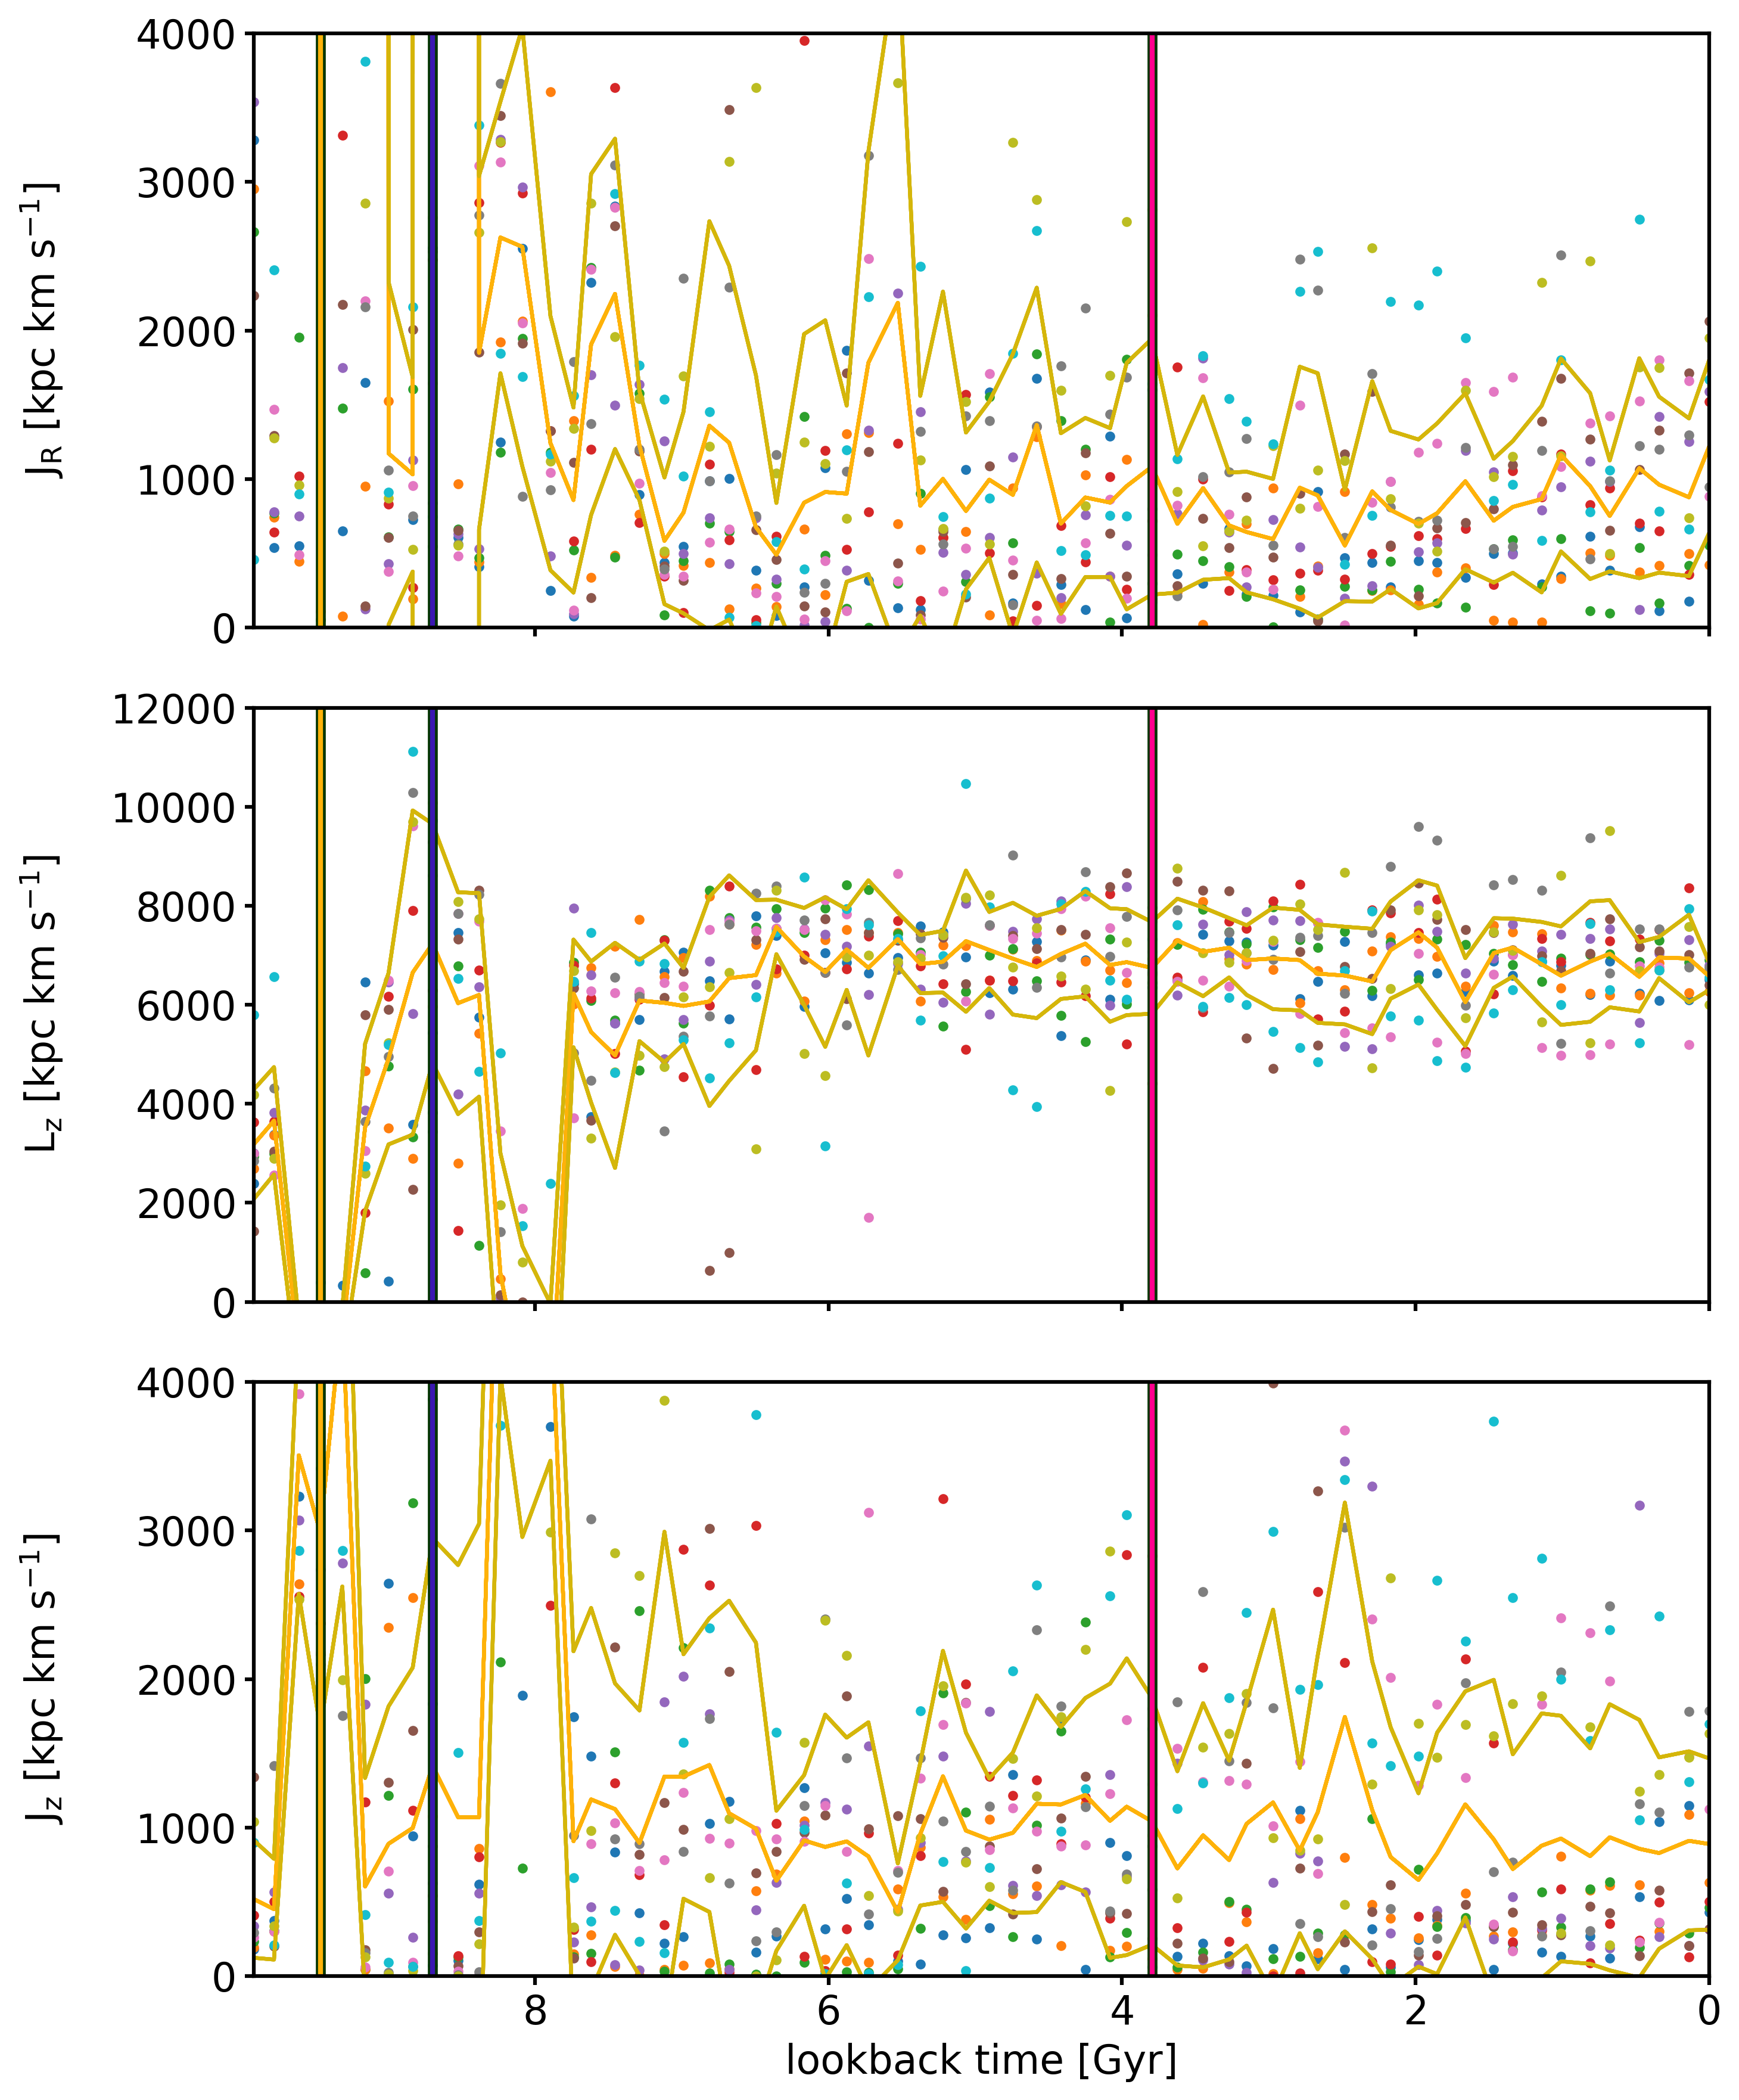
\includegraphics[width=\textwidth]{plots/Dynamics/prog4/action_time_evolution_box_hist_mean.png}
    \caption{Action time evolution of xx particles of prog4 which are on as similar orbits as possible. }\label{fig:actions_box_time_evolution_prog4}
\end{figure}
